\documentclass[11pt]{article}
\usepackage{debulletin,times,graphicx,url}

% this is the template for an issue of the Data Engineering Bulletin

% all packages used by any paper must be listed here
\usepackage{subfig}
\usepackage{listings}
\usepackage{caption}
\usepackage{microtype}
\usepackage{listings}
\usepackage{booktabs}
\usepackage{listings}
\usepackage{xargs}
%\PassOptionsToPackage{hyphens}{url}
%\usepackage{hyperref}
\usepackage{multirow}
\usepackage{tabularx}
\usepackage{makecell}
\usepackage{arydshln}
\usepackage{xspace}
\usepackage{tcolorbox}
\usepackage{xpatch}

\newcommand{\Hypercallback}{Hyperupcall\xspace{}}
\newcommand{\hypercallback}{hyperupcall\xspace{}}
\newcommand{\hide}[1]{}

\begin{document}


% please enter real date, vol no, issue no
\bulletindate{March 2019}
\bulletinvolume{42}
\bulletinnumber{1}
\bulletinyear{2019}

% these are files that I have- but your part of the issue can be done without
% them
%\IEEElogo{../../debpub/logos/cs.eps}
%\insidefrontcover{../../debpub/editors/incvA2.ps}
%\insidebackcover[ICDE Conference]{./calls/icde-new-a.ps}

\begin{bulletin}

% the above samples assume the issue is generated from a directory structure of the following sort
% major directory name is month and year of issue
% there are sub-directorys for
% letters: directory name is "letters"
% technical articles: a directory per paper, named for an "author"
% news articles: directory name is "news"
% calls: directory name is "calls

%
%  Editor letters section.  Use the lettersection environment.
%  Each letter is contained in a letter environment, where the two required
%  options to \begin{letter} are the author and the address of the author.
%

\begin{lettersection}

% there will be other letters- and a blank page will appear in your document
% but the special issue part will be fine

\begin{letter}{Letter from the Editor-in-Chief}
{Haixun Wang}{WeWork Corporation}
%\input{letters/eic-letter.tex}
\end{letter}
%
\newpage
%
%% your introductory letter goes here
%
\begin{letter}{Letter from the Special Issue Editor}
{Philippe Bonnet}{IT University of Copenhagen}
%\input{letters/editor-letter.tex}

\end{letter}

\end{lettersection}

% put the name of your special issue below

\begin{articlesection}{Cross-Layer Support for Database Management}
%
%  Contributed articles section.  Use the articlesection environment.
%  Each article is contained in an article environment, where the two required
%  options to \begin{article} are the title and author of the article
% typically, an article is stored in a directory named with one of the author names, and is then "input" into the issue
%
\begin{article}
{From the Application to the CPU: Holistic Resource Management for Modern Database Management Systems}
{Stefan Noll, Norman May, Alexander B\"{o}hm, Jan M\"{u}hlig, Jens Teubner}
\graphicspath{{submissions/snoll/figs/}}
\documentclass[11pt]{article}

\usepackage{deauthor,times,graphicx}
%\graphicspath{{noll/}}

\usepackage{subfig}
\usepackage{listings}
\usepackage{hyperref}


%\graphicspath{{./}}










\begin{document}
\title{From the Application to the CPU: Holistic Resource Management for Modern Database Management Systems}
\author{%
{Stefan Noll{\small$~^{\#+*}$}, Norman May{\small$~^{\#}$}, Alexander B\"{o}hm{\small$~^{\#}$}, Jan M\"{u}hlig$~^{+}$, Jens Teubner{\small$~^{+*}$} }
\vspace{1.2mm}\\
\fontsize{10}{10}\selectfont\rmfamily\itshape
$^{\#}$\,SAP SE, Germany\\
\fontsize{9}{9}\selectfont\ttfamily\upshape
\{stefan.noll,norman.may,alexander.boehm\}@sap.com
\vspace{1.6mm}\\
\fontsize{10}{10}\selectfont\itshape
$^{+}$\,Databases and Information Systems Group, TU Dortmund University, Germany\\
\fontsize{9}{9}\selectfont\ttfamily\upshape
jan.muehlig@tu-dortmund.de\\
\fontsize{9}{9}\selectfont\ttfamily\upshape
jens.teubner@cs.tu-dortmund.de
\vspace{1.6mm}\\
\fontsize{10}{10}\selectfont\itshape
$^{*}$\,Informatik Centrum Dortmund e.V., Germany
}
\maketitle

\begin{abstract}
With their capability to perform both high-speed transactional processing and complex analytical workloads on the same dataset and at the same time, Operational Analytics Database Management Systems give enormous flexibility to application developers.
Particularly, they allow for the development of new classes of enterprise applications by giving analytical insights into operational data sets in real time.
From a database system point of view though, these applications are very demanding, as they exhibit a highly diverse combination of  different query workloads with inhomogeneous performance and latency requirements.
In this article, we discuss the practical implications and challenges for database architects and system designers. We propose solutions that---by sharing semantics between the application, the database system, the operating system, and the hardware---allow to manage complex and resource-intensive workloads in an efficient and holistic way.
\end{abstract}



\section{Introduction}
Driven by the idea of enabling both transactional processing as well as real-time analytical query workloads in the context of a single system~\cite{nollhrm19:Plattner:2009:ACA}, a new class of database management systems has emerged, referred to as operational analytics database management systems~\cite{nollhrm19:Boehm:2016:OAD}.
These systems envision to simplify the data management landscape by consolidating multiple, disparate use cases.
Consequently, they allow the creation of novel business applications which seamlessly combine both real-time analytics and transaction processing \cite{nollhrm19:Leukert:2015:TIR}.
From a database system designer's point of view, however, delivering high performance for these modern applications puts up additional challenges because their workload characteristics are highly diverse and demanding.

In particular, static workload management schemes and simple heuristics perform suboptimally considering end-to-end performance~\cite{nollhrm19:Wolf:2014:SUM}.
The reason for this is that even the same query can have different priorities from an application's point of view, depending on the context it is being executed in.
A simple primary-key based lookup operation can be issued, e.g, in the context of a \emph{mission-critical} and time-sensitive OLTP transaction such as the \emph{interactive} data entry by a business user, but also as part of a \emph{non-critical} batch transaction that runs for hours in the \emph{background}.
A complex analytical query can be sent in the context of, e.g., a \emph{scheduled} quarter-end close report (making it rather uncritical from an execution time point of view), but also as part of a \emph{user-driven}, interactive dashboard application where virtually every millisecond counts.

Motivated by these observations, we share the opinion of other researchers that individual hard- and software-solutions throughout the data processing stack fail to address the complex challenges of these systems in isolation~\cite{nollhrm19:Giceva:2013:COD, nollhrm19:Giceva:2017:COS}.
Particularly, we believe that they are best addressed by a holistic approach, and in collaboration between the application, database management system, and the underlying hardware~\cite{nollhrm19:Boehm:2015:NOT}.

\paragraph{Outline.}
This article is structured as follows.
In Section \ref{nollhrm19:sec:hana_wlm}, we discuss how to bridge the semantic gap between the application and the database system.
Communicating additional workload context information and priorities allows the database system to perform prioritization, scheduling, and resource management that is in line with the expectations of the application.
Next, Section \ref{nollhrm19:sec:cpu_cache_partitioning} discusses a similar technique which allows the database system to share semantic information about data access patterns with the underlying hardware (i.e., the processor) by using CPU cache partitioning.
This enables the more efficient utilization of CPU caches, specifically for heterogeneous, highly concurrent workloads.
In Section \ref{nollhrm19:sec:dbms_os}, we highlight different approaches for database management systems to interact with the operating system, e.g., to improve scaling and robustness.
While commercial database systems usually choose to circumvent the OS exploiting detailed workload information, another strategy is bringing the database system and the operating system closer together with a radical co-design.
We conclude the article in Section \ref{nollhrm19:sec:conclusion}.



\section{Workload Management in SAP HANA}
\label{nollhrm19:sec:hana_wlm}

Analytical and transactional workloads do not only have different resource demands, they are also linked to different performance expectations.
\emph{Transactional} workloads are characterized by operations which consume relatively little memory and compute power.
However, they are usually sensitive to lock contention.
Unfortunately, this resource contention leads to fluctuations in statement response times, while applications expect predictable throughput and response time characteristics.
In our experience, customers are willing to sacrifice peak performance in return for better predictability of statement response times.
\emph{Analytical} workloads, on the other hand, typically are demanding regarding CPU and memory consumption.
In particular, single analytical ad-hoc statements may consume excessive amounts of memory or CPU.
This is particularly problematic for operational analytics DBMS when demanding analytical statements take away CPU clock cycles and slow down concurrent transactional workloads~\cite{nollhrm19:Wolf:2014:SUM}.

To balance or prioritize different workloads and to comply with a \emph{service level agreement} (SLA), commercial DBMS usually employ \emph{workload management} to manage resources available to single statements, applications or database users, see~\cite{nollhrm19:Zhang:AWLM:2014} for a good overview.
In SAP HANA, workload management works on a fine-grained level~\cite{nollhrm19:HANA:2018:AdminGuide} because the system is optimized for modern multi-core architectures with extensive multi-threading~\cite{nollhrm19:Psaroudakis:2015:SUC:2824032.2824043}.
Limiting, e.g., the number of working threads or the amount of memory available to the engine, can be managed for entire workloads or individual statements.
While this creates a powerful tuning option for the user, the system has to track and enforce resource consumption in all of its components.
In the following, we briefly present two mechanisms for implementing workload management using the example of SAP HANA: \emph{workload classes} and \emph{admission control}.

\paragraph{Workload Classes.}
In SAP HANA \emph{workload classes} address 1) the requirement of avoiding the excessive resource consumption of single statements and 2) the requirement of isolating the resource demands of different applications, database users, etc.\@
Workload classes are containers of configuration parameters like priority, query timeout, limits of memory consumption, or limits of concurrency per statement or per group of statements.
They are defined in the database catalog and can be applied to all statements of a database connection.
Workload classes depend on context information passed by the client application: session variables, key-value pairs maintained per database connection, e.g., \texttt{APPLICATION="ETL"}.
This context information is matched to a \emph{workload mapping} which defines the set of session variables to consider and the mapping to a workload class.

The example in Listing~\ref{nollhrm19:lst:workload_classes} defines a workload class \texttt{ETLWorkloadClass}.
Statements executed in the context of this workload class may not consume more than $5\,\mathrm{GB}$ of memory and will not use more than one thread.
The corresponding workload mapping \texttt{ETLWorkloadMapping} will apply this workload class if the session variable \texttt{APPLICATION="ETL"} is set in the database connection.
We have confirmed in many customer scenarios that workload classes can significantly help to achieve high performance and robust system behavior.

\begin{lstlisting}[
caption={Simple example of using workload classes in SAP HANA.},
captionpos=b,
label=nollhrm19:lst:workload_classes,
language=SQL,
basicstyle=\ttfamily,
]
CREATE WORKLOAD CLASS "ETLWorkloadClass"
   SET 'STATEMENT MEMORY LIMIT' = '5',
       'STATEMENT THREAD LIMIT' = '1';

CREATE WORKLOAD MAPPING "ETLWorkloadMapping"
       WORKLOAD CLASS "ETLWorkloadClass"
   SET 'APPLICATION NAME' = 'ETL'; 
\end{lstlisting}

\paragraph*{Experimental Results.}
\begin{figure}
\centering
\includegraphics[bb=0 0 317 178]{figure1.pdf}
\caption{Average response time of web requests with and without using workload classes.}
\label{nollhrm19:plt:wlm_jmeter}
\end{figure}
Figure~\ref{nollhrm19:plt:wlm_jmeter} illustrates how workload classes can improve response time of web requests in peak load situations.
We measure the average response time per web request: 
Using JMeter we issue continuously 50 web requests per second.
In addition, we slowly increase analytical and ETL load by adding five queries to each workload every five minutes.
Eventually, we reach a very high system load with close to $100\,\mathrm{\%}$ CPU utilization.
Using workload classes, we limit the ETL and the analytical workload to one thread and $5\,\mathrm{GB}$ of main memory per SQL query (cf. Listing~\ref{nollhrm19:lst:workload_classes}).
Thus, the ETL and analytical load is handled using a best-effort strategy with reduced resource usage.
The results demonstrate that enabling workload class management keeps the average response time of the web requests at a low, predictable value.

\begin{figure}
\centering
\includegraphics[bb=0 0 427 178]{figure2.pdf}
\caption{Request processing in SAP HANA using admission control.}
\label{nollhrm19:fig:hana_admission_control}
\end{figure}

\paragraph{Admission Control.}
Workload classes influence the resource consumption during execution when a statement was already admitted by the database processes.
However, a reasonably sized system may still experience short peaks in CPU or memory consumption that may result in contention of memory, CPU or latches.
Hence, in SAP HANA we complement workload classes with an \emph{admission control} mechanism.
A schematic overview is depicted in Figure~\ref{nollhrm19:fig:hana_admission_control}.

The admission control mechanism maintains a weighted moving average $z_i$ for all monitored resources of the host such as CPU utilization or total memory consumption.
When SAP HANA receives a new database request, it checks the weighted moving average against thresholds for each resource.
If each $z_i$ is below its corresponding queuing threshold $q$, the statement is admitted for immediate execution.
If the statement cannot be executed immediately, each $z_i$ is checked against its corresponding reject threshold $r$.
If the resource usage is below the reject threshold, the statement is queued; otherwise it is rejected immediately.
SAP HANA periodically checks if the resource consumption has decreased below the queuing threshold.
When this is the case, a batch of requests is fetched from the queue and scheduled for execution.
Database requests may also be rejected when the queue exceeds a configurable size or when the request is queued for too long.

Admission control samples the current resource usage $x_i$ every second.
The value $x_i$ is taken into account with, e.g., a weight of $\lambda = 0.7$.
Note that the sampling interval in combination with the weighted moving average lessens the impact of peak load situations, while the thresholds assure that the system reaches a high load without being overloaded.
In addition, admission control assumes that the client application implements a reasonable strategy to retry rejected database requests.
We could verify in productive setups that admission control helps to avoid contention issues in peak load situations, and that customers profit from a more robust system behavior.

\paragraph*{Conclusion.}
Different workloads have different resource demands and performance characteristics.
To manage hardware resources efficiently or to comply with SLAs of various workloads, commercial systems employ \emph{workload management}.
Using SAP HANA as an example, we present two techniques.
\emph{Workload classes} limit, e.g., the amount of memory or number of threads for an entire workload or an individual statement by enforcing limits across all components of the DBMS.
In addition, \emph{admission control} manages incoming request before they are admitted into the system, monitors CPU and memory consumption, and ultimately accepts or rejects a request to improve response times in peak load scenarios.



\section{CPU Cache Partitioning}
\label{nollhrm19:sec:cpu_cache_partitioning}

Modern microprocessors feature a sophisticated hierarchy of caches to hide the latency of memory access.
However, multiple cores within a processor usually share the same last-level cache (LLC).
We observed that this can hurt performance and predictability, especially in concurrent workloads whenever a query suffers from cache pollution caused by another query running on the same processor: the throughput of cache-sensitive operators may degrade by more than $50\,\mathrm{\%}$~\cite{nollhrm19:Noll:2018}.
In particular, some workloads are highly sensitive to the available amount of CPU cache (e.g., random accesses to a small hash table), contrary to cache-insensitive operations such as a sequential scan of a large memory area.
The good news is that hardware manufacturers allow fine-grained control of cache allocation by offering mechanisms such as Intel's \emph{Cache Allocation Technology} (CAT) \cite{nollhrm19:Intel:2015:CAT:whitepaper}.
By integrating a cache partitioning mechanism, which partitions the cache for individual database operators, into the execution engine of a prototype version of SAP HANA, we were able to improve the overall system performance by up to $38\,\mathrm{\%}$.

\paragraph*{Cache-Sensitivity.}
We analyzed the cache-sensitivity of individual operators using the example of the \emph{column scan} operator, the \emph{aggregation with grouping} operator and the \emph{foreign key join} operator. 
Our results show that \emph{column scans} do not profit from a large LLC.
This observation does not come as a surprise because, by nature, scans read data exactly once from DRAM without re-using it.
\emph{Aggregations}, by contrast, can be highly sensitive to the size of the LLC.
The algorithm that we consider is based on hashing, and is most cache-sensitive whenever the size of the hash tables is comparable to the (configured) LLC size.
Only if the hash table is either very small or very large, cache sensitivity becomes less significant.
Finally, the cache sensitivity of \emph{foreign key joins} heavily depends on the input data, i.e., the cardinality of the primary keys:
If the size of the bit vector used internally is comparable to the size of the cache, the algorithm becomes cache-sensitive.
Otherwise the operator does not profit from a large LLC.

\paragraph*{Cache Partitioning.}
Traditionally, the user has little control over the cache, as it is entirely managed by hardware.
Techniques such as \emph{page coloring}~\cite{nollhrm19:Lee:2009:MMC:1687627.1687670} offer the possibility of partitioning the cache by allocating memory in specific memory pages, known to map to a specific portion of the cache.
But those techniques require significant changes to the OS and the application.
Plus, re-partitioning the cache at runtime requires copying the data~\cite{nollhrm19:4658653, nollhrm19:Zhang:2009:TPP:1519065.1519076}.

\begin{figure}
\centering
\includegraphics[bb=0 0 260 140]{figure3.pdf}
\caption{Interaction between the execution engine of SAP HANA, the Linux kernel and the processor.}
\label{nollhrm19:fig:hana_cat}
\end{figure}

With the microarchitecture codenamed ``Haswell'' Intel introduced \emph{Cache Allocation Technology} (CAT) \cite{nollhrm19:Intel:2015:CAT:whitepaper} to partition the \emph{last-level cache} of a processor.
We use the Linux kernel interface of CAT (available since version 4.10~\cite{nollhrm19:Intel:2017:CAT:Kernel}) to integrate cache partitioning into the execution engine of a prototype version of SAP HANA\@.
A schematic overview of how we retrofitted cache partitioning into an execution engine is illustrated in Figure \ref{nollhrm19:fig:hana_cat}.

The execution engine of SAP HANA uses a thread pool of worker threads to execute \emph{jobs}~\cite{nollhrm19:Psaroudakis:2015:SUC:2824032.2824043}, e.g., an operator.
We annotate a job with information of its \emph{cache usage}.
The approach is similar to \emph{workload classes}, but its granularity differs.
While \emph{workload classes} annotate entire queries, the cache partitioning mechanism annotates jobs, internal units of work often featuring a distinctive memory access pattern.
Currently, we distinguish between three categories of jobs:
\textit{(i)} jobs which are not cache-sensitive and pollute the cache such as the \emph{column scan};
\textit{(ii)} jobs which are cache-sensitive and profit from the entire cache such as the \emph{aggregation with grouping} operator for most cases; and
\textit{(iii)} jobs such as the \emph{foreign key join} operator which can be both cache-polluting and cache-sensitive depending on the query or data.
By default, a job belongs to \textit{(ii)} to avoid regressions.
During the execution of a job, the engine maps a job to a bitmask and passes the bitmask and the TID of the worker thread to the Linux kernel.
The Linux kernel associates the bitmask with the TID allowing it to update a core's bitmask during thread scheduling.
Integrating cache partitioning into the code base of an industry-strength system, described into more detail in~\cite{nollhrm19:Noll:2018}, requires only a small effort: our actual implementation consists of less than 1000 lines of code.

While we derived the cache partitioning scheme from an experimental analysis, the application of existing characterization methods for \emph{describing} the cache usage pattern of a database operator could be investigated.
For instance, Chou and DeWitt~\cite{nollhrm19:Chou:1985:EBM:1286760.1286772} propose the query locality set model based on the knowledge of various patterns of queries to allocate buffer pool memory efficiently.
Others propose the cache miss ratio as an online model for characterizing workloads or operators~\cite{nollhrm19:Tam:2009:RAL:1508244.1508259, nollhrm19:Manegold:2002:GDC:1287369.1287387, nollhrm19:Zhou:2004:DTP:1024393.1024415}.

\paragraph*{Experimental Results.}
Figure~\ref{nollhrm19:plt:scan_aggregate} illustrates some of our experimental results.
Our evaluation confirms that, e.g., \emph{aggregations} are sensitive to \emph{cache pollution} caused by, e.g., \emph{column scans}.
Aggregations are most sensitive to cache pollution whenever the size of their performance-critical data structures is comparable to the size of the LLC (cf. Figure~\ref{nollhrm19:plt:scan_aggregate}b).
Note that columns in SAP HANA are dictionary-compressed.
A compressed column contains indexes which reference values in a dictionary.
A dictionary is a sorted, unique sequence of the actual domain values.
Because the \emph{aggregation} operator decompresses its input to compute the aggregate, it performs many random accesses to the dictionary of the aggregated column.
Moreover, \emph{aggregations} frequently access hash tables used for grouping.

We observed that the throughput of the \emph{aggregation} query may drop below $60\,\mathrm{\%}$ compared to running isolated in the system.
By utilizing cache partitioning and restricting the \emph{column scan} to $10\,\mathrm{\%}$ of the available LLC, we can improve the throughput of the \emph{aggregation} query by up to $21\,\mathrm{\%}$.
In addition, the \emph{column scan} operator profits from the fact that the \emph{aggregation} operator consumes less memory bandwidth:
The throughput of the \emph{column scan} increases slightly by up to $6\,\mathrm{\%}$, too.
We determine that the overall cache hit ratio increases and that the LLC misses per instruction decrease because the \emph{aggregation} performs fewer accesses to main memory and more accesses to the cache.

While the \emph{column scan} operator always pollutes the cache, other operators such as the \emph{join} operator (not shown here) only cause cache pollution whenever its frequently accessed data structures fit in the L1 or L2 cache~\cite{nollhrm19:Noll:2018}.
In these cases, we can eliminate cache pollution as well and significantly improve performance by restricting the \emph{join} to a small portion of the LLC.
Generally, the search for the ``best'' partitioning in any given situation will depend on accurate \emph{result size estimates}.

\begin{figure}
\centering
\includegraphics[bb=0 0 460 151]{figure4.pdf}
\caption{%
Throughput of Query~A (\emph{aggregation with grouping}) and Query~S (\emph{column scan}) when executed concurrently (normalized to their throughput when running isolated).
We vary the size of the dictionary of the aggregated column, we vary the number of groups, and we
disable or enable cache partitioning.
}
\label{nollhrm19:plt:scan_aggregate}
\end{figure}

\paragraph{Conclusion.}
In-memory database operators exhibit different performance characteristics depending on the available cache size.
We demonstrate how to integrate a cache partitioning mechanism into the execution engine of an existing DBMS with low expenditure and show in our evaluation that our approach avoids cache pollution and significantly reduces cache misses improving overall system performance.
Ultimately, our results illustrate that integrating cache partitioning into a DBMS engine is worth the effort: it may improve but never degrades performance for arbitrary workloads containing scan-intensive, cache-polluting operators.



\section{Interaction with the OS}
\label{nollhrm19:sec:dbms_os}

The interaction of the database management system with the operation system is crucial for achieving high concurrency, high scalability and robust performance.
While commercial database systems usually choose to circumvent the OS and exploit detailed workload information, another strategy is bringing the database system and the operating system closer together with a radical co-design.
First, we discuss how a database management system may take control of memory management and task scheduling using the example of SAP HANA\@.
Second, we present concepts as well as first experimental results for the bare metal runtime \emph{MxKernel}, a shared platform for implementing crucial components for both the DBMS and the OS. 


\subsection{Bypassing the OS}
\label{snollhrm19:sec:bypassing_os}

Instead of relying on the operating system, SAP HANA takes care of, e.g., the memory management and task scheduling itself---similar to other vendors such as IBM~\cite{nollhrm19:IBM:2004:DB2Memory} and Oracle~\cite{nollhrm19:Oracle:2018:Memory}---to achieve high concurrency, high scalability and robust performance.
In the following, we briefly present how SAP HANA ``bypasses'' the OS using the example of memory management and task scheduling.

\paragraph*{Memory Management.}
In contrast to general-purpose allocators which do not scale to thousands of cores and usually specialize in allocating small blocks, the memory management of SAP HANA is specifically built for the needs of a database system.
It is primarily optimized for high concurrency and scalability in multithreaded and NUMA environments and provides robust performance for the  allocation of different sizes of memory requests and their defragmentation (compaction and garbage collection) during the long operating time of the system (cf.~\cite{nollhrm19:Oukid:2017:MMT:3137628.3137629}).
In addition, the tailor-made implementation supports tracking and monitoring memory operations to provide fine-grained memory usage statistics.
This facilitates limiting the memory consumption globally, per instance, per process, or SQL statement for, e.g., the implementation of workload classes from Section~\ref{nollhrm19:sec:hana_wlm}.
Furthermore, the memory statistics can be used for debugging memory leaks or memory corruption as well as for analyzing performance characteristics related to memory usage.

The memory management pre-allocates memory by requesting chunks of memory (using \texttt{mmap}) from the operating system.
From this point on, the OS is no longer involved.
The cached memory is distributed across different memory pools and completely managed by the database system.
To reduce lock conflicts, each CPU has its own pool.
However, pools can still take memory from other pools.


\paragraph*{Task Scheduling.}

The task scheduling mechanism of SAP HANA utilizes its domain-specific knowledge of database internals to efficiently schedule tasks for highly concurrent, both analytical and transactional workloads.
To mitigate the problem of blocking tasks in transactional workloads, the task scheduler dynamically adapts the number of threads in the self-managed thread pool and prioritizes short-running OLTP queries.
At the same time, the scheduler makes use of a dynamic concurrency hint for analytical workloads, which results in a lower number of tasks for OLAP queries avoiding synchronization, communication and scheduling costs~\cite{nollhrm19:PsaroudakisSMA13}.
In general, the task scheduler relies on the scheduler of the Linux kernel to map threads to cores, but it, e.g., manages the thread placement to NUMA nodes explicitly and supports task stealing to deal with under-utilization~\cite{nollhrm19:Psaroudakis:2016:AND:3015274.3015275}.





\subsection{DB/OS Co-Design}
Most DBMS such as SAP HANA implement, e.g., their own memory management or task scheduling to achieve high concurrency, high scalability as well as robust performance.
Bypassing the OS comes at a price, however.
First, the DBMS re-implements features already existing in the OS.
This means that program code may be duplicated, which in return creates unnecessary maintenance and development costs.
In addition, with the OS and the DBMS having their own implementations it becomes increasingly difficult to share information.
Hence, the DBMS might have detailed information about its workloads, but at the same time it lacks the comprehensive hardware and system information available to the OS and vice versa.
Second, bypassing the OS works best if the DBMS is the only application.
However, as soon as the DBMS is co-running with another application on the same machine, e.g., in a cloud scenario or an on-premise infrastructure, dynamically managing a machine's hardware resources becomes very difficult.

A solution could be the introduction of a central component to which each application as well as the OS communicate their resource demands.
Such a component could then possess detailed information about each of the applications' workloads running on the OS \emph{and} about the OS itself.
Consequently, a radical \emph{co-design} of OS and DBMS (as well as other applications) could address the problem of dynamic resource management on a shared machine.
A first step into this direction is the bare-metal platform \emph{MxKernel}, which we introduce in the following.

\paragraph*{Architecture of MxKernel.}
Usually, DBMS are built on top of an underlying OS which is used to abstract the machine's hardware such as CPU architectures or complex memory hierarchies.
This abstraction can result in the loss of information relevant to the DBMS.
For example, applications running on top of the OS have less knowledge about parallel executed applications, the load factor of the machine and the actual hardware structure.
Using external libraries like \texttt{libnuma}~\cite{nollhrm19:kleen2005numa} might help to gain additional hardware information such as local and remote memory areas or the NUMA distribution of CPU cores.
But the use is more like a crutch and does not solve the problem holistically.
It remains, e.g, difficult to explore and utilize cache hierarchies or topology structures of various modern hardware~\cite{nollhrm19:Giceva:2013:COD}.

\begin{figure}
\centering
\includegraphics[bb=0 0 169 190]{figure5.pdf}
\caption{%
MxKernel provides a small basis layer for managing shared hardware resources between all applications running on a shared machine, including, e.g., the OS and the DBMS.
}
\label{nollhrm19:plt:mxkernel}
\end{figure}

A first step towards solving these problems in a holistic way is the bare-metal platform MxKernel.
Figure \ref{nollhrm19:plt:mxkernel} depicts an overview of the architecture.
The platform's core is a basis layer, which enables to run all applications as well as the OS side by side.
Note that running an OS is optional.
At the same time, MxKernel provides a detailed view of the hardware and an interface to which an application can communicate its requirements regarding hardware resources or performance expectations.

In particular, it implements services for hardware compatibility and a mechanism for control flow execution.
Moreover, its architecture allows, e.g., the OS and the DBMS to share data structures and algorithms such as B-Trees, which can be used for primary key indexing by the DBMS or for implementing a file system by the OS.

\paragraph*{MxTasks.}

The platform MxKernel introduces \emph{MxTasks} to abstract from and to create an interface to the control flow execution.
MxTasks describe small units of work representing a more lightweight alternative to POSIX Threads.
They are executed atomically by implementing a run-to-completion semantic.
Usually, MxTasks feature only a small sequence of instructions.
As a result, their runtime, memory accesses, and resource requirements are easier to predict and to define than threads.
In addition, MxTasks can be coupled with precise metadata about, e.g., its memory access patterns, its accessed data structures and its preferred NUMA region.
Thus, by annotating \emph{MxTasks} with workload information we employ the same concept of sharing semantics between application, OS, DBMS, and hardware as discussed for \emph{workload classes} in Section~\ref{nollhrm19:sec:hana_wlm} or for \emph{jobs} in Section~\ref{nollhrm19:sec:cpu_cache_partitioning}.

MxKernel creates an execution plan that synchronizes MxTasks for shared-resource accesses and optimizes them for cache and NUMA locality.
Thus, MxKernel functions as a central component for resource management which receives (workload) information in the form of MxTasks with metadata.
Its execution framework then tries to fulfill the requirements of all applications as well as possible.
Applications running on top of an (optional) OS, however, can still choose to use threads instead of MxTasks for compatibility reasons.

Furthermore, MxTasks represent a way to exploit heterogeneous systems by providing different implementations for distinct processing units such as GPUs or CPUs.
Based on system load and the runtime property of a MxTask, MxKernel could then choose the most suitable available hardware for execution.

\paragraph*{Experimental Results.}
As a first use case, we evaluated an index data structure based on the B\textsuperscript{link}-tree~\cite{nollhrm19:Lehman:1981:ELC:319628.319663}.
We implement the insert algorithm described by Lehman and Yao~\cite{nollhrm19:Lehman:1981:ELC:319628.319663}.
However, we modify it to support MxTasks: We spawn a new task for each traversal of a node.
This means that we create a task for looking up the child node to traverse next.
When a task finally finds the matching leaf node, we insert the new value.

While concurrent POSIX Threads accessing the same node of the B\textsuperscript{link}-tree have to be protected using latches, MxTasks benefit from the run-to-completion semantic:
Mapping the traversal of a tree node to a specific processor core ensures that only one task accesses a node at a time.
In addition, we benefit from cache locality because one core accesses the same data structure multiple times.

\begin{figure}
\centering
\includegraphics[bb=0 0 317 211]{figure6.pdf}
\caption{Throughput of insert operations into a B\textsuperscript{link}-tree. While the throughput drops down when using more than four POSIX Threads, the throughput stagnates when using MxTasks from the second NUMA region.}
\label{nollhrm19:fig:blinktree:results}
\end{figure}

We consider two different implementations of the B\textsuperscript{link}-tree: a version based on POSIX Threads executed on Linux, and a version based on MxTasks running on MxKernel.
The workload consists of $16 \cdot 10^6$ insert operations using unique key-value pairs.
We execute the experiment on a system with two Intel Xeon E5-2690 processors with 8 CPU cores each, and simultaneous multithreading enabled.

The results illustrated in Figure \ref{nollhrm19:fig:blinktree:results} show that while the thread-based version exhibits a higher throughput until using eight threads, the throughput starts dropping after using four threads.
We explain the differences with the latch contention of the thread version:
Every node has to be protected by a latch to prevent inconsistencies.
MxTasks, on the other hand, have no need to use latches.
Every node of the B\textsuperscript{link}-tree is assigned to one of the cores and every MxTask accessing a node will be executed on the mapped core without suspension.

In addition, we notice that the throughput degrades slightly after using cores from the second NUMA node.
We attribute this to the increased overhead of cache coherency.
For managing MxTasks and tracking their execution state, we use a wait-free queue for every core.
Pushing MxTasks from a queue of one core to the queue of another core, triggers the cache coherency mechanism of the processor which costs additional execution time.
This effect occurs as soon as another NUMA node is involved.
Note that the throughput of the thread-based version, on the other hand, drops significantly with more than 16 cores.


\paragraph*{Conclusion.}
The interaction between DBMS and OS are crucial for creating high-performance systems.
We briefly present how a commercial system such as SAP HANA bypasses the OS and implements, e.g., its own memory management and task scheduling to guarantee robust performance and scaling by exploiting domain-specific knowledge, or to track and to enforce the consumption of hardware resources.
Another strategy is the co-design of DBMS and OS.
As a first step towards this goal, we introduce the bare-metal platform \emph{MxKernel}.
On top of it, the DBMS and the OS run side by side with an interface to communicate their hardware and runtime requirements to.
In return, MxKernel manages hardware resources exclusively.



\section{Conclusion}
\label{nollhrm19:sec:conclusion}

Operational analytics database management systems with the capability to perform both high-speed transactional processing and complex analytical workloads on the same dataset and at the same time, impose new challenges and practical implications for system designers.
In this article, we discussed several solutions that allow to manage these resource-intensive workloads in an efficient and holistic way.
In particular, we explicitly share workload information between application, OS, DBMS, and hardware which allows us to manage resources efficiently and to improve performance and predictability.

By sharing context information between the application and the DBMS, systems can implement an application-aware resource management and quality of service features.
SAP HANA employs \emph{workload classes} for limiting the resource consumption of queries issued by individual applications.
In addition, we presented its \emph{admission control} mechanism to manage the amount of requests the system handles at a given time in order to avoid contention in peak load situations.

By sharing cache usage information between the DBMS and the hardware, we implement a mechanism that \emph{dynamically partitions} the \emph{cache} per individual operator.
We demonstrated that this may improve the overall throughput of highly concurrent workloads, where we restrict the cache usage of scan-intensive operators and increase the cache capacity for cache-sensitive operators.

Finally, we discussed how the database system interacts with the operating system.
While DBMS traditionally take control over individual features of the OS and implement, e.g., a custom memory management or task scheduling, other research directions explore their co-design.
In particular, we presented the bare-metal platform \emph{MxKernel}.
On top of it, the DBMS and the OS run side by side and communicate their hardware and runtime requirements to the platform.
In return, MxKernel takes care of managing all hardware resources.

\section*{Acknowledgments}
This work was supported by DFG, Deutsche Forschungsgemeinschaft, grant number TE 1117/2-1.




\begin{thebibliography}{10}
\itemsep=1pt
\begin{small}
\bibitem{nollhrm19:Plattner:2009:ACA}
H.~Plattner. \newblock A Common Database Approach for OLTP and OLAP Using an In-Memory Column Database. \newblock \emph{SIGMOD}, 2009, pp. 1--2.

\bibitem{nollhrm19:Boehm:2016:OAD}
A.~B{\"{o}}hm, J.~Dittrich, N.~Mukherjee, I.~Pandis, and R.~Sen. \newblock Operational Analytics Data Management Systems. \newblock \emph{VLDB}, vol.~9, no.~13, pp.
1601--1604, 2016.

\bibitem{nollhrm19:Leukert:2015:TIR}
H.~Plattner and B.~Leukert. \newblock The In-Memory Revolution: How SAP HANA Enables Business of the Future. \newblock Springer, 2015.

\bibitem{nollhrm19:Wolf:2014:SUM}
I.~Psaroudakis, F.~Wolf, N.~May, T.~Neumann, A.~B{\"{o}}hm, A.~Ailamaki, and
K.~Sattler. \newblock Scaling up Mixed Workloads: a Battle of Data Freshness, Flexibility, and Scheduling. \newblock \emph{TPCTC}, 2014, pp. 97--112.

\bibitem{nollhrm19:Giceva:2013:COD}
J.~Giceva, T.~Salomie, A.~Sch{\"{u}}pbach, G.~Alonso, and T.~Roscoe. \newblock COD: Database / Operating System Co-Design. \newblock \emph{CIDR}, 2013.

\bibitem{nollhrm19:Giceva:2017:COS}
K.~Kara, J.~Giceva, and G.~Alonso. \newblock FPGA-based Data Partitioning. \newblock \emph{SIGMOD}, 2017, pp. 433--445.

\bibitem{nollhrm19:Boehm:2015:NOT}
A.~B{\"{o}}hm. \newblock Novel Optimization Techniques for Modern Database Environments. \newblock \emph{BTW}, 2015, pp. 23--24.

\bibitem{nollhrm19:Zhang:AWLM:2014}
M.~Zhang. \newblock Autonomic Workload Management for Database Management Systems. \newblock \emph{Ph.D. thesis}, Queen's University, 2014.

\bibitem{nollhrm19:HANA:2018:AdminGuide}
\mbox{SAP SE}.\hspace{1mm}\mbox{SAP HANA Administration Guide}.\hspace{1mm}\url{https://help.sap.com/viewer/6b94445c94ae495c83a19646e7c3fd56/2.0.03/en-US}, 2018.

\bibitem{nollhrm19:Psaroudakis:2015:SUC:2824032.2824043}
I.~Psaroudakis, T.~Scheuer, N.~May, A.~Sellami, and A.~Ailamaki. \newblock Scaling Up Concurrent Main-Memory Column-Store Scans: Towards Adaptive NUMA-aware Data and Task Placement. \newblock \emph{VLDB}, vol.~8, no.~12, pp. 1442--1453,
2015.

\bibitem{nollhrm19:Noll:2018}
S.~Noll, J.~Teubner, N.~May, and A.~B\"{o}hm. \newblock Accelerating Concurrent Workloads with CPU Cache Partitioning. \newblock \emph{ICDE}, 2018,
pp. 437--448.

\bibitem{nollhrm19:Intel:2015:CAT:whitepaper}
Intel Corporation. \newblock Improving Real-Time Performance by Utilizing Cache Allocation Technology. \newblock \emph{White paper}, 2015.

\bibitem{nollhrm19:Lee:2009:MMC:1687627.1687670}
R.~Lee, X.~Ding, F.~Chen, Q.~Lu, and X.~Zhang. \newblock MCC-DB: Minimizing Cache Conflicts in Multi-core Processors for Databases. \newblock \emph{VLDB},
vol.~2, no.~1, pp. 373--384, 2009.

\bibitem{nollhrm19:4658653}
J.~Lin, Q.~Lu, X.~Ding, Z.~Zhang, X.~Zhang, and P.~Sadayappan. \newblock Gaining Insights into Multicore Cache Partitioning: Bridging the Gap Between Simulation and Real Systems. \newblock \emph{HPCA}, IEEE Computer Society, 2008, pp. 367--378.

\bibitem{nollhrm19:Zhang:2009:TPP:1519065.1519076}
X.~Zhang, S.~Dwarkadas, and K.~Shen. \newblock Towards Practical Page Coloring-based Multicore Cache Management. \newblock \emph{EuroSys}, ACM, 2009, pp. 89--102.

\bibitem{nollhrm19:Intel:2017:CAT:Kernel}
Intel Corporation. \newblock User Interface for Resource Allocation in Intel Resource Director Technology. \newblock Documentation of the Linux Kernel, \url{https://www.kernel.org/doc/Documentation/x86/intel_rdt_ui.txt}, 2017.

\bibitem{nollhrm19:Chou:1985:EBM:1286760.1286772}
H.-T. Chou and D.~J. DeWitt. \newblock An Evaluation of Buffer Management Strategies for Relational Database Systems. \newblock \emph{VLDB}, 1985, pp. 127--141.

\bibitem{nollhrm19:Tam:2009:RAL:1508244.1508259}
D.~K. Tam, R.~Azimi, L.~B. Soares, and M.~Stumm. \newblock RapidMRC: Approximating L2 Miss Rate Curves on Commodity Systems for Online Optimizations. \newblock \emph{ASPLOS}, ACM, 2009, pp.
121--132.

\bibitem{nollhrm19:Manegold:2002:GDC:1287369.1287387}
S.~Manegold, P.~Boncz, and M.~L. Kersten. \newblock Generic Database Cost Models for Hierarchical Memory Systems. \newblock \emph{VLDB}, 2002, pp. 191--202.

\bibitem{nollhrm19:Zhou:2004:DTP:1024393.1024415}
P.~Zhou, V.~Pandey, J.~Sundaresan, A.~Raghuraman, Y.~Zhou, and S.~Kumar. \newblock Dynamic Tracking of Page Miss Ratio Curve for Memory Management. \newblock \emph{ASPLOS}, ACM, 2004, pp.
177--188.

\bibitem{nollhrm19:IBM:2004:DB2Memory}
IBM. \newblock The DB2 UDB memory model -- How DB2 uses memory. \newblock \url{https://www.ibm.com/developerworks/data/library/techarticle/dm-0406qi/}, 2018.

\bibitem{nollhrm19:Oracle:2018:Memory}
Oracle. \newblock Database Administrator’s Guide -- Managing Memory. \newblock \url{https://docs.oracle.com/database/121/ADMIN/memory.htm}, 2018.

\bibitem{nollhrm19:Oukid:2017:MMT:3137628.3137629}
I.~Oukid, D.~Booss, A.~Lespinasse, W.~Lehner, T.~Willhalm, and G.~Gomes. \newblock Memory Management Techniques for Large-Scale. Persistent-Main-Memory Systems. \newblock \emph{VLDB}, vol.~10, no.~11, pp. 1166--1177, 2017.

\bibitem{nollhrm19:PsaroudakisSMA13}
I.~Psaroudakis, T.~Scheuer, N.~May, and A.~Ailamaki. \newblock Task Scheduling for Highly Concurrent Analytical and Transactional Main-Memory Workloads. \newblock \emph{ADMS}, 2013, pp. 36--45.

\bibitem{nollhrm19:Psaroudakis:2016:AND:3015274.3015275}
I.~Psaroudakis, T.~Scheuer, N.~May, A.~Sellami, and A.~Ailamaki. \newblock Adaptive NUMA-aware Data Placement and Task Scheduling for Analytical Workloads in Main-Memory Column-Stores. \newblock \emph{VLDB}, vol.~10, no.~2, pp. 37--48, 2016.

\bibitem{nollhrm19:kleen2005numa}
A.~Kleen. \newblock A NUMA API for Linux. \newblock \emph{White paper}, SUSE Labs, 2004.

\bibitem{nollhrm19:Lehman:1981:ELC:319628.319663}
P.~L. Lehman and S.~B. Yao. \newblock Efficient Locking for Concurrent Operations on B-Trees. \newblock \emph{ACM Trans. Database Syst.}, vol.~6, no.~4, pp. 650--670, 1981.
\end{small}
\end{thebibliography}

\end{document}

\end{article}
%
\begin{article}
{Leveraging Hyperupcalls To Bridge The Semantic Gap: An Application Perspective}
{Michael Wei, Nadav Amit}
\graphicspath{{submissions/mwei/figs/}}
\documentclass[11pt]{article} 


%%%%%%%%%%%%%%set margin to 1in

%%%%%%%%%%%%%%%%%%%%

\usepackage{amsmath}
\usepackage{verbatim}
\usepackage{comment} 
\usepackage{algorithm}
\usepackage{algorithmic}
\usepackage{amsfonts}
\usepackage{amssymb}
%\usepackage{amsmath}
\usepackage{subfig}
\usepackage{multirow}
\usepackage{flushend}
\usepackage{caption}
\usepackage{url}
%\usepackage{xspace}
%\usepackage{xcolor}
%\usepackage{enumitem,url}
\usepackage{deauthor,times,graphicx}

\usepackage{bbm}




\newcommand{\ceil}[1]{\left\lceil{#1}\right\rceil}
\newcommand{\floor}[1]{\left\lfloor{#1}\right\rfloor}

\newcommand{\remove}[1]{}

\newcommand{\bbone}{\mathbbm{1}}
\newcommand{\cK}{{\mathcal  K}}
\newcommand{\cS}{{\mathcal  S}}

\newcommand{\degrees}{$\!\!$\char23$\!$}
\DeclareFontFamily{OT1}{psyr}{}
\DeclareFontShape{OT1}{psyr}{m}{n}{<-> psyr}{}
\def\times{{\fontfamily{psyr}\selectfont\char180}}

%\newtheorem{definition}{Definition}
%\newtheorem{example}{Example}
\newtheorem{problem}{Problem}
\newcommand{\hide}[1]{}


\renewcommand{\refname}{\centerline{References}}

% this handles hanging indents for publications
\def\rrr#1\\{\par
\medskip\hbox{\vbox{\parindent=2em\hsize=6.12in
\hangindent=4em\hangafter=1#1}}}

\def\baselinestretch{1.01}

\begin{document}
\title{Fairness and Robustness in Answering Preference Queries}

\author{
Senjuti Basu Roy\\
New Jersey Institute of Technology\\
senjutib@njit.edu}


\date{}

\maketitle
\begin{abstract}

Given a large number of users preferences as inputs over a large number of items, preference queries leverage different preference aggregation methods to aggregate individual preferences in a systematic manner and come up with a single output (top-$k$ ordered or unordered/a complete order) that is most representative. The preference aggregation methods are widely adopted from the social choice theory, some of which are rank based (single-round vs. multi-round), while others are non-rank based. These queries are prevalent in high fidelity applications, including search, ranking and recommendation,  hiring and admission, and electoral voting systems. This article outlines algorithmic challenges and directions in designing an optimization guided computational framework that allows to change the original  aggregated output (either ordered or unordered top-$k$ or a complete order) to satisfy different criteria related to {\em fairness and robustness}, considering different preference elicitation models (ways users provide their input preferences) and aggregation methods (ways the individual preference get aggregated). 


\end{abstract}


\vspace{-0.1in}
\section{Introduction}
\vspace{-0.1in}
The need to aggregate a large number of individual preferences in a  systematic manner is {\em ubiquitous}. Users can provide preferences in many ways - as likes/dislikes, ordinal preferences, or ranked order (full or partial). The social choice theory~\cite{feldman2006welfare} offers a plethora of aggregation methods to aggregate individual preferences and come up with a single output. These outputs may be a single rank that is most representative of all users preferences, or sometimes a smaller number of $k$ items (top-$k$) that are ordered or  presented as a set. While  designed for electoral voting systems primarily, the applicability of answering queries is prevalent in many high fidelity applications, such as, ranking and listing web search results, recommending movies/songs,  selecting a handful of candidates for domains where resource is scarce (such as hiring and admission), to name a few. It is not a stretch to consider a setting in which thousands of items (notationally $n$) have received preferences from hundreds of thousands (or even millions) of users (notationally $m$) and the goal is to produce a single output (notationally $\sigma$) that is most {\em representative}. 



The computational implications of different preference aggregation methods are well studied. {\em What is not so well understood is how hard it is to change the original produced output, which may be necessary for many compelling reasons.}  Satisfying additional criteria, such as, promoting fairness (e.g., ensuring presence of individuals with certain socio-demographic properties),  or Understanding robustness, i.e., figuring out the minimum amount of change of the inputs that would result in a different outcome than the original output. This latter aspect provides understanding on how manipulable the proposed aggregation methods are which are certainly important for aggregation methods that are heavily used in electoral systems, but are applicable in other scenarios as well (e.g., in figuring out the robustness of a rating system of products). To the best of our knowledge, {\em a systematic study is needed to investigate these aspects in conjunction with different preference elicitation models, requiring different preference aggregation methods.} That, in nutshell, is the focus of this article.

%While our focus is studying how to change the original output of the preference aggregation methods that may be necessary for different reasons, 
\smallskip \noindent We discuss these challenges considering four interspersed dimensions, as described below.

\smallskip \noindent {\em \bf Preference Elicitation Models.}
The article simultaneously considers a vast range of preference elicitation processes that we broadly categorize as rank based and non rank based. In rank based processes, the users can provide a fully ranked order over all items, a partial order, or a coarser preference (like item a ranked higher than item b, etc). In non rank based preferences, users can provide only likes, both likes and dislikes, or even an ordinal preference (likes item a as "excellent", b as "good", etc). The choice of these preference elicitation methods is dictated by the different applications. Rank based ones are suitable in hiring/admission/electoral system, while non rank based ones are more relevant in obtaining user feedback from search results, user satisfaction survey, product reviews, etc.

\smallskip \noindent {\em \bf Preference Aggregation Methods.}
Then the preference aggregation methods that are most commensurate to the underlying preference elicitation process and underlying application are studied. For example, when user preferences are given as ranked order, depending on the underlying application, we will aggregate them using existing single-round rank based methods  (e.g., Kemeny, Spearman's footrule, or Borda), or multi-round based methods (STV, IRV). The former aggregation methods are suitable in hiring decision, whereas, the latter ones are gaining popularity in voting systems. On the other hand, when users provide non rank based preferences, we will show how Jaccard similarity or Hamming distances are suitable to aggregate them and come up with the final output. 

\smallskip \noindent {\em \bf Produced Output Form.}
From the application point of view, the produced output may require an order over all $n$ items (hiring/admission), or a small number $k$ of $n$ items as outputs. In case of top-$k$ items requirement, the returned $k$-items may need to be ordered for certain applications  (top-$k$ web pages returned by the search engine), or in some cases it is fine to return them as a set (selecting a set of representatives or body to form certain committee). 

\smallskip \noindent {\em \bf Change Original Output.}
The importance of quantifying the minimum effort needed to change the original output is evident for several reasons, such as  promoting fairness and robustness. Robustness is heavily used in {\em electoral system} to produce {\em margin},  that investigates how to bound the amount of change of the original outcome in case x\% of the inputs are destroyed/deleted/modified. We discuss them further in details below.
%\begin{itemize}
 %   \item {\bf Promoting additional criteria.} It is highly desirable in many compelling applications to produce outputs that satisfy additional criteria (e.g., fairness, diversity) while staying as close as possible to the original output.
  %  \item {\bf Study robustness.} In many practical applications, especially ones related to voting and electoral system, there is a need to understand the following question. How to bound the amount of change of the original outcome in case x\% of the inputs are destroyed/deleted/modified. This problem relates to finding {\em margin} in electoral system, which intends to figure out how much change is needed in the original input to even minimally change the original outputs. 
%\end{itemize}



%\smallskip \noindent {\bf Proposed Project.} 
%The project will be executed based on three broadly defined aims. %The first part of the proposal will study different preference elicitation models of the members , with the objective of producing fairness aware~\cite{zehlike2021fairness,verma2018fairness,chairman, pfair,layard2008social,amer2009group,berkovsky2010group} preference aggregation models. The outcomes of this objective are formalism/models that incorporate fairness with preference aggregation and studies a wide spectrum of variants.  Then, we  focus on the computational aspect of the proposed problems - investigate their hardness, and propose efficient solutions with provable guarantees. Our efficiency consideration shall also investigate how to reuse the current computation if the inputs come dynamically and over time. Finally, we will demonstrate how to enable actionable fair preference aggregation in two compelling applications including electoral voting systems (such as ranked choice voting~\cite{rank1,rank2}) and perform additional experimental evaluation for qualitative and computational efficacy. 

%\smallskip \noindent{Research challenges.}

\vspace{-0.1in}
\section{Overarching Research Goals}
\vspace{-0.1in}
The overarching goal is to design optimization guided computational framework containing principled models and scalable solutions that allows to change the original  aggregated output  (either ordered or unordered top-$k$ or a complete order) to satisfy different criteria, considering different  preference elicitation models and aggregation functions to promote:  \textbf{a.~Fairness} from the standpoint of the protected attributes\cite{verma2018fairness} of the items/candidates  %as well as of the members
(e.g., race, gender, ethnicity), where the candidates are selected by aggregating elicited preferences of the members (panelists, voters, search committee). We shall investigate existing group fairness criteria in the context of preference aggregation~\cite{zehlike2021fairness,verma2018fairness}, as well as adapt fairness criteria studied in the context of resource allocation or social choice theory.  \textbf{b.~Robustness}, namely, understanding how easy or hard it is to change the original outcome of different preference aggregation models given a budgeted preference substitution requirement. For instance, if the total number of preference updates is budgeted to be $\leq x$, is it possible to change the original outcome? 
 We are interested in exploring these viewpoints for multiple preference elicitation models and output forms.  What is also important to notice is that a given preference elicitation may be suitable to multiple aggregation methods and may require to satisfy more than one produced output form. These gives rise to many combinations of the problem.

%Our long term vision is the ambitious goal of developing a computational framework that is flexible enough to accommodate any domain expert defined criteria to minimally change the outcome of any existing preference aggregation protocol to promote additional criteria that are commensurate to new rules and policies, as well as present efficient and automated computations of outcomes.
%To realize these contributions, we propose to develop a computational framework containing a suite of principled models by formalizing multiple ways of changing outcomes of initial preference aggregation solutions considering individual preference elicitation models that are suitable to a wide variety of compelling applications and design efficient solutions for those. 


\smallskip \noindent The rest of the article is organized as follows:
\smallskip \noindent In Section~\ref{aim1}, we study how to Satisfy output constraints in single round rank-based preference aggregation methods.
We study this considering ranking, which is a commonly used method to prioritize  desirable outcomes among a set of items/candidates and is an essential step in  many high impact applications. Here the members elicit a {\em complete or partial preference order} over the candidates and the goal is to produce an aggregated ranked order over all candidates or produce top-$k$ results that minimize disagreements  among individual preferences. 
We will also include preference substitution in single round rank-based preference aggregation methods to satisfy {\em complex} top-$k$  constraints, where the  requirement is defined over a set $R$ of protected attributes. 
%Handling multiple protected attributes is applicable when the fairness  requirements span several dimensions like gender, race, age, (genre, language, actors for movie results diversification) etc. Recent work~\cite{bartl2020unmasking,blodgett2020language,snob2023} shows that even in case of a single fairness attribute such as gender, it may be necessary to implement multiple fairness requirements since considering only the single fairness attribute seldom accounts for within-group heterogeneity and biases that may disproportionately affect some members of a group. %This will require extension of recent works~\cite{islam2022satisfying} in which preference substitution is studied in a simple plurality voting setting. %The computational problem is defined as follows- {\em find margin via single ballot substitutions to promote a set of $k$ candidates as top-$k$, considering  multiple protected attributes of the candidates}. 
%Previous approaches for handling fairness requirement over multiple protected attributes assumed that these attributes are independent and thus the multiple attributes can be translated into a single fairness attribute defined over the Cartesian product of the attributes' domains. However, as shown in~\cite{islam2022satisfying} this assumption may be too restrictive. 
%In this setting the ranking is determined by tallying ballots each of which is for a single candidate. The objective is to {\em minimize the number of single ballot substitutions that guarantee the satisfaction of the complex fairness constraints in the top-$k$ results}. In voting theory~\cite{cary2011estimating}, the concept of margin of victory (MOV) is designed to measure electoral competitiveness of the candidates, that is formalized as the smallest number of single ballot substitutions to promote a given set of $k$ candidates as the top-$k$. To the best of the PIs' knowledge, they are one of the first to formalize the computational problem - {\em find margin via single ballot substitutions to promote a set of $k$ candidates as top-$k$, considering  multiple protected attributes of the candidates}. Previous approaches for handling fairness requirement over multiple protected attributes assumed that these attributes are independent and thus the multiple attributes can be translated into a single fairness attribute defined over the Cartesian product of the attributes' domains. However, as shown in~\cite{islam2022satisfying} this assumption may be too restrictive. 


\smallskip \noindent In Section~\ref{aim2}, we study how to satisfy output constraints in multi round rank-based preference aggregation methods, popularly known as ranked choice voting or (RCV)~\cite{irv1}. Two popular representatives of these models are IRV (Instant run-off voting)~\cite{irv1} that selects one item/candidate as the winner, and STV (single transferable vote)~\cite{stv-irv, stv1} that generalizes IRV and selects a set of $k$-items/candidates as winners.  It is known that RCV represents majority rules and improves result diversity. Unlike single round preference aggregation models, RCV minimizes the effect of {\em strategic voting} as users can provide their ``true preference'' for the candidates they support, not just provide preference against the items/candidates they oppose most. It is also shown in recent works, how RCV promotes anonymity and anti-plurality~\cite{stv-irv}, compared to single round based algorithms.
%For completeness, we describe the (simpler) IRV process:  If an item/candidate receives more than half of the first-choice votes, then this item/candidate wins, exactly as they would in ``plurality based'' single round process. If there’s no majority winner, then the process is decided by an ``instant runoff'' - The candidate who has the fewest votes is eliminated; users who had chosen that item/candidate as their first choice have their second choice counted instead. This process is iterated until a winner representing more than half of the votes emerges. It is known that RCV represents majority rules and improves result diversity. Unlike single round preference aggregation models, RCV minimizes the effect of {\em strategic voting} as users can provide their ``true preference'' for the candidates they support, not just provide preference against the items/candidates they oppose most. It is also shown in recent works, how RCV promotes anonymity and anti-plurality~\cite{stv-irv}, compared to single round based algorithms.

%The initial users preferences are elicited as ranked order up to ballot size $t$. We will first adopt IRV model  and study how easy or hard it is to select the winner candidate/item from a predefined set. In applications where such selections are repeated this will be used to promote  different notions of fairness and diversification, as described  in Section~\ref{aim2}. We will continue then to study STV which is a multi-winner extension of IRV and selects top-$k$ items/candidates. Optimizing preference substitution in multi round voting schemes is hard to compute. A known result in this space shows that it is NP-Hard to determine whether the outcome of an IRV can be swayed by adding just a single preference~\cite{stv2}. For STV we considered the simplest scenario when every user is allowed to rank just two items/candidates, namely their top choice and their second best. We were able to show that even in this seemingly simple setting it is NP-Hard to determine the minimum number of preference substitutions needed to change the outcome. We will study these problems considering different output criteria/constraints, as discussed in Section~\ref{aim2}.

\smallskip \noindent In Section~\ref{nonrank}, we will study how to satisfy output constraints in non rank based preference aggregation methods.
Here we investigate preference aggregation methods that do not require users inputs to be ranked order. A simple case in this context is a Boolean model, where each user describes their preference over $n$ items as a Boolean vector of $0$ and $1$. When users provide only their ``likes'' on the items, the aggregation function such as Jaccard Similarity or Overlap similarity~\cite{roy2014exploiting} may be appropriate to find top-$k$ items that have exhibited maximum similarity over the users preferences. On the other hand, when the users provide both ``likes'' and ``dislikes'', the aggregation function may intend to produce a Boolean vector that minimizes the Hamming Distance between the input preferences and the produced output. Generalization of the Boolean preference elicitation models is also discussed.

%Akin to the previous two sections, here also we intend to study how to change original output to satisfy fairness and robustness based criteria in the output. Even when the output criteria is ``simple'' (refer to Section~\ref{preliminary} for details), we anticipate these problems to become computationally intractable  for Hamming Distance. On the other hand, we conjecture these problems to be polynomial time computable for overlap similarity. Understanding how to change the original output under simple and complex output criteria will be studied thoroughly under this aim for both Boolean and Ordinal preference aggregation models.

%For all three sections, we will first study suitable formalism/models, study their complexity analytically, following which we will intend to design scalable solutions with provable guarantees. %Our efficiency consideration shall also investigate how to reuse the current computation if the inputs come dynamically and over time.

%\smallskip \noindent In  Section~\ref{eval}, we will further layout plans on how to deploy such framework to enable actionable interventions in real world applications. \textbf{A.}~Given additional criteria (either an existing notion of fairness, or a domain expert provided criteria) adapt popular ranking/recommendation models (such as multi-arm bandit, or matrix factorization), understand and evaluate  the efficacy of the proposed computational framework in promoting that criteria as well as their computational effectiveness. \textbf{B.}~ Given a predefined budget of manipulations, which aggregation models are vulnerable to change the outcome vs. which ones are not. 

%For the first approach, in collaboration with a domain expert and their provided criteria  (collaboration letter attached), we plan to analyze the New York Times annotated corpus (https://paperswithcode.com/dataset/new-york-times-annotated-corpus) to understand news article recommendation to different users. We will also study a popular electoral voting system, namely, the Ranked Choice Voting (RCV in short)~\cite{rank1, rcv1, rcv2, rcv3, rcv4} for selecting council members or committee.  We intend to follow the mechanism used in Cambridge MA and used their publicly available data~\cite{RCV} to elect its city council as described in~\cite{rcvdesc}. For the second approach we plan to evaluate robustness of large scale tweet, movie rating, and product rating datasets considering various preference elicitation and aggregation models.

%\noindent {\bf Novelty.}  The exclusivity introduced by our project hinges on $5$ key facets: \textbf{A.}~study individual preference elicitation models; \textbf{B.}~adapt a suite of preference aggregation functions (single round and multi-round) that are commensurate to different preference elicitation models to produce ordered or unordered top-$k$ or a full order; \textbf{C.}~allow domain experts to define criteria (considering fairness, diversification, and robustness) and propose formalism to change the original outcome based on that;  \textbf{D.}~investigate principled models and algorithms that minimally modify the output produced by the the aggregation models to satisfy the additional criteria, while producing total or top-$k$ results; \textbf{E.}~demonstrate the applicability of the framework in multiple key applications. 

%\noindent {\bf High Level Research Challenges.}
%The first and foremost research challenge is to propose/ adapt fairness models that are suitable for preference aggregation. Then, one  key research challenge of the project lies in developing a suite of models (optimization problems) that suitably combine different fairness and preference elicitation criteria and aggregate them to produce a single complete order or top-$k$ results (either ordered or unordered). As an example, one possible extreme is  to produce a result that is optimal for preference aggregation subject to being strictly fair. Contrarily, one can design an order that combines fairness as a weight inside preference aggregation functions. We shall investigate these alternatives as part of this challenge.  The next key challenge is computational - that is, design algorithms that  scale on very large datasets, and exhibit theoretical guarantees. As an example, one of the simplest form of preference aggregation, namely the rank aggregation~\cite{dwork2001rank}
%problem is known to be NP-Complete, where the inputs contain multiple complete or partial orders of preferences from a set of members and the output is a single ranked order that minimizes disagreement among individual orders, considering a variety of distance measures, such as, Kendall-Tau or Spearman's Footrule Distance. We shall investigate if existing algorithmic frameworks for rank aggregation~\cite{ailon2008aggregating,ailon2010aggregation} adapt to solve rank aggregation considering fairness. We will study how to perform preference aggregation considering fairness when the input preferences are {\em qualitative} (e.g., Member 1 prefers Molly and Amy; Abigail, Kim, and Lee are acceptable; and the remaining ones must not be considered) . We are keen to design solutions where the input data is dynamic, i.e., all individual preferences are not present at the same time. Our last and final key challenge is to  operationalize our proposed framework to recommend actionable interventions.

%\begin{wrapfigure}{r}{0.65\textwidth}
 %%  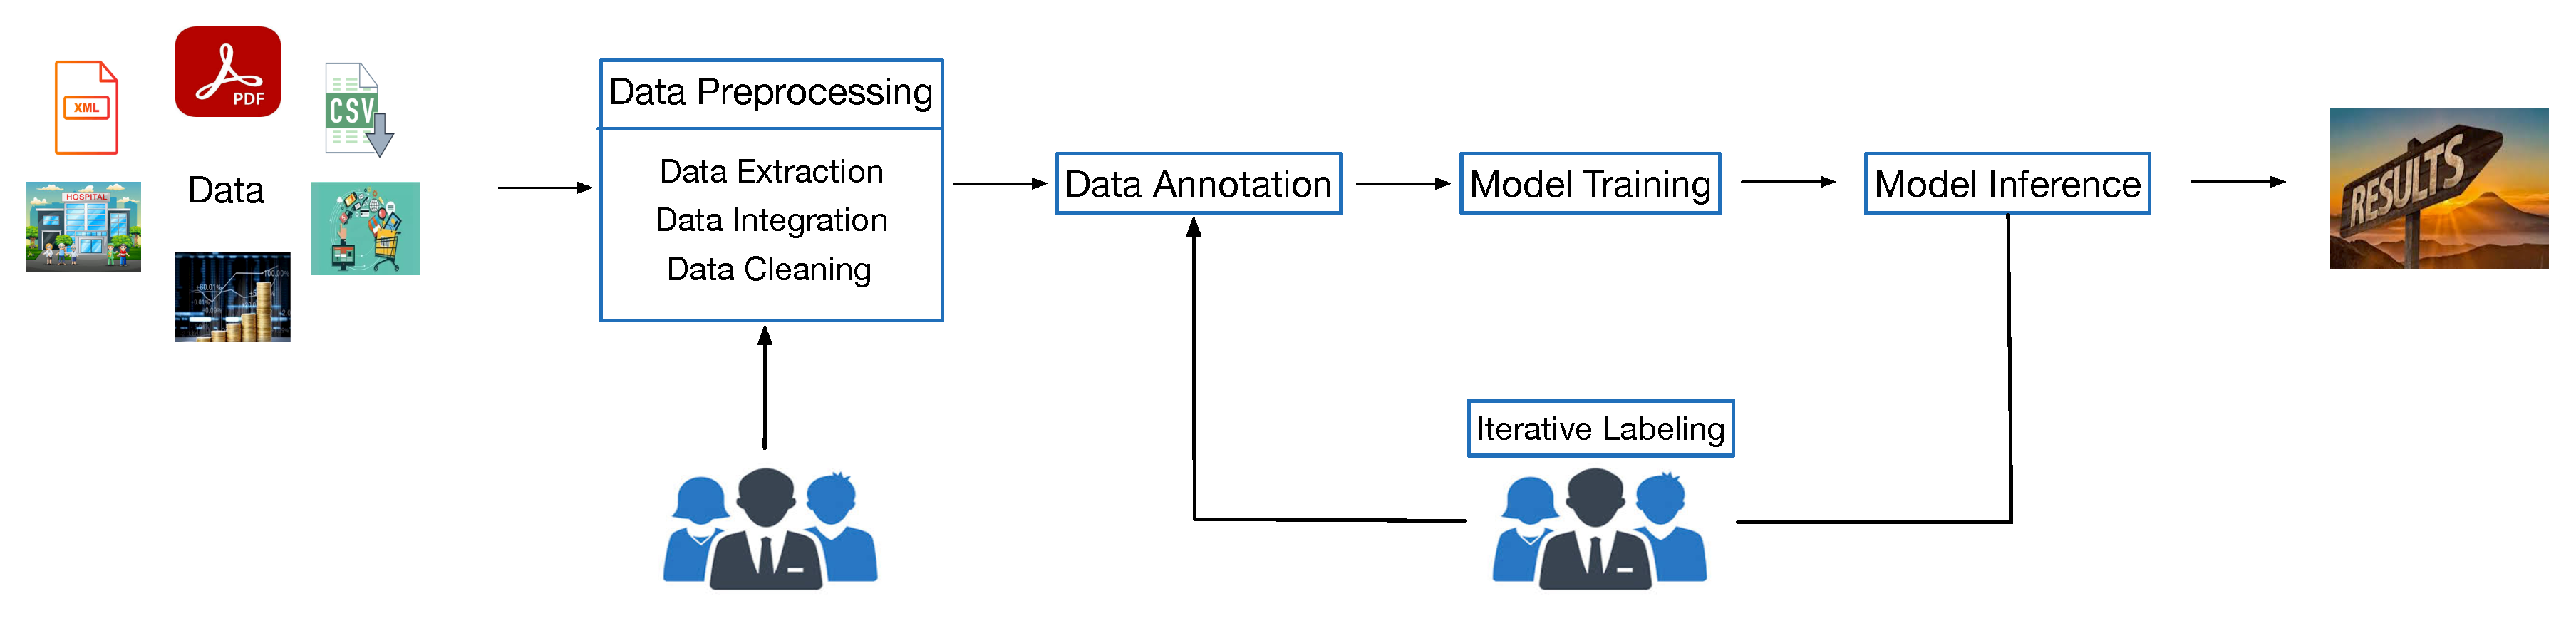
\includegraphics[width=0.65\textwidth]{
%NSFcore-2023/framework.pdf}
 %%\caption{Proposed Project}\label{project}
%\end{wrapfigure}



%We intend to propose complete, partial (either order or unordered), and various qualitative individual preference elicitation models.  An example of the first two would be having complete or only top-$k$ order of preferences over the candidates as inputs, whereas, an example of the last one  would be to bucketize candidates in different qualitative groups (recall the motivating example). For fairness, our effort would be to design group based fairness criteria designed over the protected attributes of the candidates that resemble group fairness criteria, such as, demographic parity, or statistical parity, studied in the context of classification~\cite{verma2018fairness}. To that end, we will adapt proportionate-fairness or p-fairness~\cite{pfair,chairman}  from resource allocation theory that ensures proportionate representation of every group based on a protected attribute in every position of the produced results, or its generalization~\cite{amer2009group} adapted from the social choice theory to promote affirmative action~\cite{fu2006theory} in the produced results.  
%Preference aggregation would be studied considering Kendall-Tau and Spearman's Footrule Distance functions~\cite{kemeny,diaconis1977spearman}, with the objective to minimize the sum of disagreement (Kemeny Optimization) or such, akin to existing {\em (fairness unaware) classical rank aggregation problem}~\cite{dwork2001rank,ailon2008aggregating, ailon2010aggregation}. Our goal would be to make these solutions fairness aware by investigating how to combine these two somewhat conflicting aspects in a systematic manner. For each of these proposed problem variants, we shall analyze the nature of the problem analytically and design scalable solutions with theoretical guarantees. Finally, we will perform both qualitative and quantitative study to develop actionable interventions by leveraging our proposed framework to promote fairness in two compelling applications: (i) Ranked Choice Voting (RCV)~\cite{rcv1,rcv2}, and (ii) Gender and diversity gap in the Oscars. We intend to fine-tune our proposed models based on these evaluations. 

\noindent {\bf Comparison with Existing Work.}
This contribution builds on our work recent works on fairness~\cite{islam2022satisfying, wei2022rank}, and prior works on preference aggregation~\cite{amer2009group, amer2015group, basu2015group}, studying robustness~\cite{roy2014exploiting}. We acknowledge that the existing popular group based fairness definition, such as, {\em statistical parity}~\cite{dwork2012fairness} is somewhat similar to one of our proposed fairness notion. However, the best adapted version of top-$k$ statistical parity studied in a recent paper~\cite{vldbrank} does not account for proportionate representation in every position of the top-$k$, limiting its applicability.  Studying computational challenges related to computing the margin of victory  has been a focus of recent research~\cite{stv1,stv2, stv3} in the context of electoral voting and related applications. But none of these existing works study the general version of the problem, which is, how to promote additional simple/complex constraints/criteria in the output, which is our primary focus. Other than these prior works, which are  much narrow in scope, we are unaware of any computational work that systematically studies different preference elicitation models, multiple output changing criteria, and preference aggregation combining these two.  

%Section~\ref{related} provides an in-depth comparison between our proposed work and existing work.  
%To the best of our knowledge, we are the first to investigate a generic framework that can minimally update original outcome of preference aggregation to satisfy complex constraints without any assumption on the relationship among the attributes.

%Using the aforementioned example, if $k=12$, existing work~\cite{vldbrank} only ensures p-fairness of the aggregated rank at position $12$, but not for the remaining positions (e.g., 1 to 11). {\em While p-fairness promotes stronger notion of fairness, and our proposed framework adapts to top-$k$ statistical parity, existing work does not adapt to our proposed optimization framework}.

%\smallskip \noindent {\bf Aim 1 - Fair Rank Aggregation.}
%We will begin our study in the context of ranking, which is a commonly used method to prioritize  desirable outcomes among a set of candidates and is an essential step in  many high impact applications. Here the members elicit a {\em complete preference order} over the candidates and the goal is to produce an aggregated ranked order over all candidates or produce top-$k$ results that minimize disagreements  among individual preferences. When fairness is studied, our goal would be to ensure fair representation of the candidates based on their one or more protected attributes (such as, gender, race, etc.) in the ranked order. 
%\smallskip \noindent {\bf Aim 2 - Fair Partial and Qualitative Preference Aggregation.}
%In this aim we shall consider scenarios where either qualitative preferences or partial rankings are elicited from the members. 
%We consider three such preferences: (1) top-$t$ ranking, where the input preference is a ranking of the top-$t$ items (candidates), (2) subset selection, where the input preference is an unordered subset of favorite elements, and (3) bucketing, where the input preference is a partition of the elements into three subsets: the ``yes'' set, ``ambivalent'' set, and the ``no'' set.  In our preliminary work, we consider the selection of council members or a committee of $k$ members from $n$ candidates considering the votes of $m$ judges (voters) ({\em ranked choice voting}~\cite{rank1} could be considered as a popular application of that).  The fairness criterion models affirmative action and includes a lower and upper bound on the number of elected candidates, for each value of the protected attributes(s). We intend to study the design choices of different preference elicitation models considering fairness, formalize the optimization problems and analyze them, and design principled solutions with guarantees.

%The mechanism we focus on to aggregate the top-$k$ rankings is {\em Ranked choice voting (RCV)}, and specifically RCV employing a single transferable vote (STV) system~\cite{rcvdesc}.
%We are going to follow the mechanism used in Cambridge MA to elect its city council. 

%\smallskip \noindent {\bf Aim 3 - Actionable Fair Preference Aggregation.}
%Although the proposed models and algorithms consider 
%fairness in its design, rather than an afterthought, the third aim will delve deeper into fairness considerations of compelling applications and develop actionable interventions. In particular, the third aim will provide a holistic large-scale study over two compelling applications and present actionable interventions to promote fairness. In the first application, we will study fairness in Ranked Choice Voting (RCV)\footnote{\small https://qz.com/1676718/the-pros-and-cons-of-ranked-choice-voting/} considering the data provided by the Cambridge, MA
%City Council Election 2019~\cite{RCV} to analytically answer important questions raised in recent research~\cite{rcv1,rcv2,rcv3, rcv4,rcv5}. 1. Does more choice lead to reduced racially polarized voting? 2. Does ranked choice voting enable minority representation?  Based on the analysis, {\em we will develop actionable interventions by leveraging our proposed framework to mitigate these risks}. We will perform both qualitative and quantitative analysis. For qualitative  analysis, we will recruit experienced workers from Amazon Mechanical Turk (the budget justification provided further details). A similar  study would be conducted to investigate the gender and diversity gap in the Academy of Motion Picture Arts and Sciences decisions by combining it with large scale Movielens~\cite{movielens} data and we will develop actionable recommendation to mitigate the gap. Further evaluation plan considering other datasets is described in Section~\ref{eval}.

%\section{Introduction}
\label{seC:intro}
% Interpretability and nutritional labels, generally

An essential ingredient of successful machine-assisted decision-making, particularly in high-stakes decisions, is interpretability --– allowing humans to understand, trust and, if necessary, contest, the computational process and its outcomes.   These decision-making processes are typically complex:  carried out in multiple steps, employing models with many hidden assumptions, and relying on datasets that are often repurposed --- used outside of the original context for which they were intended.\footnote{See Section 1.4 of Salganik's ``Bit by Bit''~\cite{salganik} for a discussion of data repurposing in the Digital Age, which he aptly describes as "mixing readymades with custommades.''}  In response, humans need to be able to determine the ``fitness for use'' of a given model or dataset, and to assess the methodology that was used to produce it.  

To address this need, we propose to develop interpretability and transparency tools based on the concept of a {\em nutritional label}, drawing an analogy to the food industry, where simple, standard labels convey information about the ingredients and production processes. Short of setting up a chemistry lab, the consumer would otherwise have no access to this information. Similarly, consumers of data products cannot be expected to reproduce the computational procedures just to understand fitness for their use.   Nutritional labels, in contrast, are designed to support specific decisions by the consumer rather than completeness of information.  A number of proposals for hand-designed nutritional labels for data, methods, or both have been suggested in the literature\cite{DBLP:journals/corr/abs-1803-09010,DBLP:journals/corr/abs-1805-03677,DBLP:conf/fat/MitchellWZBVHSR19}; we advocate deriving such labels automatically or semi-automatically as a side effect of the computational process itself, embodying the paradigm of {\em interpretability-by-design}. 

Interpretability means different things to different stakeholders, including individuals being affected by decisions, individuals making decisions with the help of machines, policy makers, regulators, auditors, vendors, data scientists who develop and deploy the systems, and members of the general public.  Designers of nutritional labels must therefore consider {\em what} they are explaining,  {\em to whom}, and {\em for what purpose}.  In the remainder of this section, we will briefly describe two regulatory frameworks that mandate interpretability of data collection and processing to members of the general public, auditors, and regulators,  where nutritional labels offer a compelling solution (Section~\ref{sec:intro:reg}).  We then discuss interpretability requirements in data sharing, particularly when data is altered to protect privacy or mitigate bias (Section~\ref{sec:intro:synth}).

\subsection{Regulatory Requirements for Interpretability}
\label{sec:intro:reg}

The European Union recently enacted a sweeping regulatory framework known as the General Data Protection Regulation, or the GDPR~\cite{gdpr}.  The regulation was adopted in April 2016, and became enforceable about two years later, on May 25, 2018.  The GDPR aims to protect the rights and freedoms of natural persons with regard to how their personal data is processed, moved, and exchanged (Article 1).  The GDPR is broad in scope, and applies to ``the processing of personal data wholly or partly by automated means'' (Article 2), both in the private sector and in the public sector.  Personal data is broadly construed, and refers to any information relating to an identified or identifiable natural person, called the {\em data subject} (Article 4).  

According to Article 4, lawful processing of data is predicated on the data subject's {\em informed consent}, stating whether their personal data can be used, and for what purpose (Articles 6, 7).
Further,  data subjects have {\em the right to be informed} about the collection and use of their data.~\footnote{\url{https://gdpr-info.eu/issues/right-to-be-informed/}}
Providing insight to data subjects about the collection and use of their data requires technical methods  that support interpretability.  

Regulatory frameworks that mandate interpretability are also starting to emerge in the US.  New York City was the first US municipality to pass a law (Local Law 49 of 2018)~\cite{Vacca}, requiring that a task force be put in place to survey the current use of ``automated decision systems'' (ADS) in city agencies. ADS are defined as ``computerized implementations of algorithms, including those derived from machine learning or other data processing or artificial intelligence techniques, which are used to make or assist in making decisions.''   The task force is developing recommendations for enacting algorithmic transparency by the agencies, and will propose procedures for: (i) requesting and receiving an explanation of an algorithmic decision affecting an individual (Section 3 (b) of Local Law 49); (ii) interrogating ADS for bias and discrimination against members of legally protected groups, and addressing instances in which a person is harmed based on membership in such groups (Sections 3 (c) and (d)); (iii) and assessing how ADS function and are used, and archiving the systems together with the data they use (Sections 3 (e) and (f)).

Other government entities in the US are following suit.  Vermont is convening an Artificial Intelligence Task Force to ``... make recommendations on the responsible growth of Vermont’s emerging technology markets, the use of artificial intelligence in State government, and State regulation of the artificial intelligence field.''~\cite{Vermont}.  Idaho’s legislature has passed a law that eliminates trade secret protections for algorithmic systems used in criminal justice~\cite{Idaho}.  In early April 2019, Senators Booker and Wyden introduced the Algorithmic Accountability Act of 2019 to the US Congress~\cite{BookerWydenClarke}. The Act, if passed, would use ``automated decision systems impact assessment'' to address and remedy harms caused by algorithmic systems to federally protected classes of people. The act empowers the Federal Trade Commission to issue regulations requiring larger companies to conduct impact assessments of their algorithmic systems.

The use of nutritional labels in response to these and similar regulatory requirements can benefit a variety of stakeholders.  The designer of a data-driven algorithmic method may use them to validate assumptions, check legal compliance, and tune parameters.  Government agencies may exchange labels to coordinate service delivery, for example when working to address the opioid epidemic, where  at least three sectors must coordinate: health care, criminal justice, and emergency housing, implying a global optimization problem to assign resources to patients effectively, fairly and transparently. The general public may review labels to hold agencies accountable to their commitment to equitable resource distribution. 


\subsection{Interpretability with Semi-synthetic Data}
\label{sec:intro:synth}

%Datasets are now increasingly used to train models to make decisions once made by humans.  In these automated systems, biases in the data are propagated and amplified with no human in the loop.  The bias, and the effect of the bias on the quality of decisions made, is not easily detectable due to the relative opacity of the system.  

A central issue in machine-assisted decision-making is its reliance on historical data, which often embeds results of historical discrimination, also known as {\em structural bias}.   As we have seen time and time again, models trained on data will appear to work well, but will silently and dangerously reinforce discrimination~\cite{propublicaJ,amazon_hiring,amazon_delivery}.  Worse yet, these models will legitimize the bias --- ``the computer said so.''  Nutritional labels for data and models are designed specifically to mitigate the harms implied by these scenarios, in contrast to the more general concept of ``data about data.''

Good datasets drive research: they inform new methods, focus attention on important problems, promote a culture of reproducibility, and facilitate communication across discipline boundaries.  But research-ready datasets are scarce due to the high potential for misuse. Researchers, analysts, and practitioners therefore too often find themselves compelled to use the data they have on hand rather than the data they would (or should) like to use.  For example, aggregate usage patterns of ride hailing services may overestimate demand in early-adopter (\ie wealthy) neighborhoods, creating a feedback loop that reduces service in poorer neighborhoods, which in turn reduces usage.  In this example, and in many others, there is a need to alter the input dataset to achieve specific properties in the output, while preserving all other relevant properties.  We refer to such altered datasets as \textit{semi-synthetic}.

Recent examples of methods that produce semi-synthetic data include database repair for causal fairness~\cite{DBLP:conf/sigmod/SalimiRHS19}, database augmentation for coverage enhancement~\cite{DBLP:conf/icde/AsudehJJ19}, and privacy-preserving and bias-correcting data release~\cite{DBLP:conf/ssdbm/PingSH17,DBLP:conf/vldb/RodriguezSPSH18}. A semi-synthetic datasets may be altered in different ways.  Noise may be added to it to protect privacy, or statistical bias may be removed or deliberately introduced.  When a dataset of this kind is released, its composition and the process by which it was derived must be made interpretable to a data scientist, helping determine fitness for use.  For example, datasets repaired for racial bias are unsuitable for studying discrimination mitigation methods, while datasets with bias deliberately introduced are less appropriate for research unrelated to fairness.   This gives another compelling use case for nutritional labels.

%To make our discussion more concrete, let us consider data scientists who must identify datasets appropriate for their task.  This is particularly important when semi-synthetic datasets are being released, to which noise is added to protect privacy, or statistical bias is removed or deliberately introduced.  For example, datasets repaired for racial bias are unsuitable for studying discrimination mitigation methods, while datasets with bias deliberately introduced are less appropriate for research unrelated to fairness.  



%\input{IEEE-data-engineering-IC1/preliminary}
\vspace{-0.2in}
\section{Formalism}\label{preliminary}
\vspace{-0.1in}
%The proposed work aims at developing an optimization guided computational framework that modifies an output obtained from a preference aggregation method applied on a preference elicitation model to produce a modified output that satisfies given criteria. The proposed work aims at developing this framework for a suite of preference elicitation models and preference aggregation methods.
%that satisfies with criteria that guides the need to change the original output minimally while producing a complete or top-$k$ (ordered or unordered) result aggregating individual preferences.

There are $4$ types of inputs that our proposed framework takes: (a)~a set $N$ of $n$ items, where each item has a set $\mathcal{A}$ of discrete attributes.  Each attribute $a\in \mathcal{A}$ has $\ell_a$ different values. (b)~a set of $m$ users, where the $i$-th user $u(i)$ provides her preference as $\sigma_i$. The users' preferences could be rank based, partial or full order, or non rank based. (c)~a distance function $\mathcal{F}$ (defined formally below) that measure the ``distance'' between a set of $m$ input preferences  $\sigma_1, \sigma_2,\ldots, \sigma_m$ and an output $\sigma$ with the required output form. The exact distance function depends on the underlying preference elicitation model and the required output form which may be either a complete ranking of the items or a subset of $k$ items, either ranked or not. (d)~a set $\mathcal{C}$ of output criteria/constraints. Some variants of our problem also include as input a budgetary constraint $B$.

%The proposed work aims at developing an optimization guided computational framework that suitably combines a suite of preference elicitation models with criteria that guides the need to change the original output minimally while producing a complete or top-$k$ (ordered or unordered) result aggregating individual preferences. %Next, we present some definitions that will be used throughout the proposal.  

\begin{definition}\label{def4}
\vspace{-0.1in}
{\bf Distance function $\mathcal{F}$.} Given $m$ input preferences  $\sigma_1, \sigma_2,\ldots, \sigma_m$ and an output $\sigma$ with the required output form, the function $\mathcal{F}(\sigma, \sigma_1, \sigma_2,\ldots, \sigma_m)$ is the distance of $\sigma$ from the input preferences  $\sigma_1, \sigma_2,\ldots, \sigma_m$.
In some cases the function $\mathcal{F}(\cdot)$ is an aggregation of a distance function between a single input preference and the output. Examples for such an aggregation are the sum of the pairwise distances and the maximum distance to any of the input preferences. In other cases $\mathcal{F}(\cdot)$ measures the minimum modification of the input preferences that would result in the preference aggregation method outputting the output $\sigma$. 
%$\mathcal{F}(\sigma, [\sigma_1, \sigma_2,\ldots, \sigma_m])$
\end{definition}

\vspace{-0.1in}
\begin{definition}\label{def1}
\vspace{-0.1in}
{\bf Output criteria/constraints.}  For an attribute $a\in \mathcal{A}$,  let $c(p_a)$ denote the cardinality constraints of items with value $p_a$ ($p_a$ is one of the $\ell_a$ possible values of attribute $a$). Given to the framework is a set $C$ of such cardinality constraints for each attribute value $p_a$, for every $a \in A$, $A \subset \mathcal{A}$. There are two explicit cases that we consider.
\begin{itemize}
    \item {\bf The output $\sigma$ is ordered and consists of $k\le n$ items.} 
    In this case the cardinality constraints are defined for every $\kappa \in [1..k]$ items, and for every  such $\kappa \in [1..k]$, the $\kappa$ top ranked items of output $\sigma$ have to satisfy these cardinality constraints.  
    %the $k$ top ranked items satisfy all cardinality constraints defined over $v$, i.e., it satisfies $c(p^v_{a_1}) \text{ AND } c(p^v_{a_2}) \text{ AND } \ldots \text{ AND } c(p^v_{a_A})$.  
     \item {\bf The output $\sigma$ is an unordered set of $k$ items.} In this case the cardinality constraints are defined for $k$ items and the items in the output set $\sigma$ have to satisfy these cardinality constraints. 
     \\ %$c(p_{a_1}) \text{ AND } c(p_{a_2}) \text{ AND }  \ldots \text{ AND } c(p_{a_A})$.  
\end{itemize}  
\end{definition}
\vspace{-0.1in}
\begin{definition}\label{def3}
\vspace{-0.1in}
{\bf A budgetary constraint.} A budgetary constraint $B$ is an upper bound on the distance of the output from the input preferences. 
%For a given distance function $\mathcal{F}(\cdot)$, 
The budgetary constraint implies that $\mathcal{F}(\sigma,\sigma_1,\sigma_2,\ldots,\sigma_m)\leq B$.  
\end{definition}

\vspace{-0.1in}
\begin{definition}\label{def2}
{\bf Preference Aggregation Considering Constraints.} 
We intend to study different types of problem definitions that require different algorithmic treatments.
Given either complete or partial preferences $\sigma_1,\sigma_2,\ldots,\sigma_m$ over the items in $N$, a preference aggregation method, a distance function $\mathcal{F}(\cdot)$, and a set of output criteria $\mathcal{C}$.
\vspace{-0.1in}
\begin{itemize}
    \item {\bf (Constrained optimization).} Produce an output $\sigma$ with the required form that minimizes $\mathcal{F}(\sigma,\sigma_1,\sigma_2,\ldots,\sigma_m)$ and satisfies $\mathcal{C}$.
    \vspace{-0.1in}
    \item {\bf (Optimization under budgetary constraints).} Produce an output $\sigma$ with the required form that optimizes $\mathcal{C}$,  while satisfying $\mathcal{F}(\sigma,\sigma_1,\sigma_2,\ldots,\sigma_m) \leq B$. (The objective function for optimizing $\mathcal{C}$ varies.)
    \vspace{-0.1in}
    \item {\bf (Bi-criteria optimization).} Given parameters $\alpha$ and $\beta$ produce an output $\sigma$ with the required form that satisfies both $\mathcal{F}(\sigma,\sigma_1,\ldots,\sigma_m) \le \alpha$ and $\mathcal{G}(\mathcal{C}) \le \beta$, where $\mathcal{G}$ is the objective function for optimizing $\mathcal{C}$.
\end{itemize}
\end{definition}
%The individual research aims will describe the various forms of preference elicitation from users and the details of the preference aggregation methods. We first delineate the need to change original output and the challenges that arise from there.
\vspace{-0.1in}
\subsection{Specifying Output Criteria}
We discuss orthogonal reasons where the original outputs coming out of the preference aggregation methods need to be ``massaged'' further. What unifies them is that these criteria are defined over one or more attributes of the items. Depending on how many attributes are involved in the definition and their relationship thereof gives rise to additional challenges.


%\vspace{-0.1in}
%\subsection{Important Concepts and Definitions}\label{pre}
%\vspace{-0.1in}
%\noindent \textbf{Database.} contains $n$ items or candidates. These two terms will be used interchangeably. The set of items will be denoted $V$, individual items will be denoted by $u$ and $v$. \\
%\noindent {\em \bf Individual preference Elicitation:} We consider the following individual preference elicitation models. \\
%\noindent (1) Complete preference: Each of the $4$ members (Judges) may provide a {\em complete order of preference} over the $12$ candidates (Refer to Table~\ref{tab:example_original_rank}). \\
%\noindent (2) Partial preference: 
%(2.1) Ordered. Member 1 (as well as other members) may provide a partial order over the first $5$ candidates and does not specify anything for the rest.\\
%(2.2) Unordered. Member 1 (as well as other members) may also specify that she likes the first $5$ candidates without specifying any order among them.\\
%\noindent (3) Qualitative Preference: Contrarily, Member 1 (as well as other members) may provide {\em qualitative preferences}: Molly and Amy are preferred, Abigail, Kim, Lee are acceptable, the remaining ones must not be considered. These are considered to be the inputs to the framework. Please note that 2.2 is a simplified variant of this last preference elicitation model.

%\noindent \textbf{Multiple Preferences.} The input consists $m$ different preference elicitation (based on the individual models described above). Using the motivating example, $m=4$.

\subsubsection{Fair Preference Aggregation}
We will study fairness in the context of group based protected attributes of the candidates. Output criteria/constraints for fairness (refer to Definition~\ref{def1}) are expressed over one or more {\em protected attributes}. Their protected attributes could be expressed over gender, ethnicity, race, or the state the candidates are living in. 

Formally speaking, each item/candidate $v\in N$ has one or more  {\em protected attributes}. When $\ell_a=2$, it is a binary protected attribute; when $\ell_a \geq 2$ it is a multi-valued protected attribute. As an example, race is (usually) a multi-valued protected attribute, and gender is sometimes a binary protected attribute.

%\begin{itemize}
%\item  {\bf p-fairness.} 
\smallskip \noindent \textbf{p-fairness.}
p-fairness has been studied in the context of resource allocation satisfying temporal fairness or proportionate progress~\cite{chairman, pfair}. It was introduced in the classical  {\em Chairman Assignment Problem}~\cite{baayen1964existence, chairman} that studies how to select a chairman of an union every year from a set of  $n$ states such that  that at any time the accumulated number of chairmen from each state is proportional to its weight. 

In the context of ranking, suppose that each of the $n$ ranked items has a {\em protected attribute} $a(\cdot)$ that can take any of $\ell_a$ different values. For $p_a\in [1..\ell_a]$, let $c'(p_a)$ denote the fraction of items with protected attribute value $p_a$, that is, $c'(p_a) = \frac 1n \sum_{i=1}^n \bbone_{a(i)=p_a}$. The goal is to ensure that $c'(p_a)$ fraction (rounded either up or down) of every top $\kappa$ items have protected attribute value $p_a$.
\iffalse
\vspace{-0.1in}
\item {\bf Generalization of p-fairness to promote affirmative action.} Instead of requiring $c'(p_a)$ fraction of every top $\kappa$ items to have protected attribute value $p_a$, we may want that certain values of the protected attribute get higher representation among the elements at the top, more than their overall proportion. Let $P$ be a non-negative doubly stochastic $n \cdot \ell_a$ matrix. The goal is to ensure that $P(\kappa,p_a)$ fractions (rounded either up or down) of the top $\kappa$ items to have value $p_a$, for every $\kappa \in [1..n]$ and $p_a\in [1..\ell_a]$ (if it is feasible).
It is not difficult to note that such a generalized notion can capture affirmative action.
%\end{itemize}
\fi


\subsubsection{Robust Preference Aggregation}
Output criteria/constraints for robustness on the other hand investigates the flip questions: Given either complete or partial preferences $\sigma_1,\sigma_2,\ldots,\sigma_m$ over $n$ items, let $\sigma$ be the output obtained by the preference aggregation method. Given a budget $B$, how to  make $B$ or less changes in the original preferences, such that the outcome is different from $\sigma$? This question is  related to finding the {\em margin} in electoral systems and quantifies how manipulable the underlying aggregation method is. We study this problem under different manipulation models -- addition only, deletion only, or substitution (addition + deletion).

\iffalse
\subsection{Challenges in Handling  Complex Output  Criteria}
In general, the output requirements/constraints are defined over a set $R$ of attributes. When $|R|=1$, as an example, the output requirement is defined on a single attribute (such as race). In a recent work, we demonstrated that for an aggregation method that models plurality voting, the problem of preference aggregation while satisfying output criteria defined by a single attribute is computationally easy. 
However, the nature of the problem changes when two or more attributes are involved in the output criteria. In Section~\ref{aim1} we discuss this more complicated case and refer to our recent work in which we showed evidence that in some cases it is computationally difficult even to find any output with the required form. 
\fi
%When there are two or more different attributes involved in outlining output criteria/constraints (such as certain representation from race and certain representation from gender), the PIs have proved in a recent work~\cite{islam2022satisfying} that the decision version of the preference aggregation problem under output constraint becomes (weakly) NP-hard by reducing the well known NP-hard Partition problem to our problem~\cite{garey1979computers}. We note that the existing practice of converting multiple attributes to a single multi-valued protected attribute by computing joint distribution over the attributes assumes independence among the attributes. When Independence among the attributes does not hold, this simplification leads to a heuristic process.  The PIs have also demonstrated that for three (or more) attributes (e.g., constraints defined over race, and gender, and ethnicity), even the question whether there exists a set of top-$k$ that satisfies the complex constraint is strongly NP-Hard where the reduction is fro 3 Dimensional Matching. On the positive side for the case of two  attributes, the PIs have designed an efficient algorithm a preference aggregation algorithm while satisfying fairness constraints defined over $2$ attributes and has designed a 2 approximation factor and runs in $O(n^2\ell \log m)$ time, by casting this problem as a min cost flow problem, where $\ell$ is the total number of possible attribute values. We intend to study these aspects in the proposal - as it turns out to be an intellectually demanding and independent  facet of the computational problem, irrespective of the specific reasons to change the output.


%\input{IEEE-data-engineering-IC1/aim1}
\vspace{-0.2in}
\section{Single Round Rank based Preference Aggregation}\label{aim1}
\vspace{-0.1in}
We outline two separate lines of algorithmic problems: (1) incorporating output criteria (e.g., p-fairness) in single round rank-based preference aggregation methods, and (2) satisfying complex constraints in single round rank-based preference aggregation methods.
\vspace{-0.1in}
\subsection{Incorporating output criteria in rank aggregation} 
\vspace{-0.1in}
The input to the classical {\em rank aggregation} problem consists of $m$ complete order of preferences over the $n$ items/candidates. Traditionally, producing the final ranking involves aggregating potentially conflicting preferences from multiple individuals, and is known as the rank aggregation problem~\cite{dwork2001rank,van2007deterministic, ailon2008aggregating}. Our goal is to  minimally change the aggregated output to enable fairness.
%p-fairness has been studied in the theory community to enable resource allocation satisfying temporal fairness or proportionate progress.
We will study p-fairness~\cite{chairman, pfair} that ensures proportionate representation of every group based on a protected attribute in every position of the aggregated ranked order.  The classical problem in this context is known as the {\em Chairman Assignment Problem}~\cite{baayen1964existence, chairman} which studies how to select a chairman of a union every year from a set of  $r$ states such that  that at any time the accumulated number of chairmen from each state is proportional to its weight. p-fairness generalizes other notions of fairness~\cite{islam2023equitable} that were considered in prior work, including the existing popular group based fairness definition {\em statistical parity}~\cite{dwork2012fairness}. 
%We start with some definitions and then describe both our preliminary research and the open problems we plan to investigate further.
\vspace{-0.1in}
\subsubsection{Research Directions}
\vspace{-0.1in}
%\noindent \textbf{Rank and Multiple Ranking.}  
Consider rankings of the items in a set $V$. Each such ranking can be viewed as a permutation. We will use the terms ranking and permutation interchangeably. 

\noindent \textbf{Kendall-Tau and Kemeny distances.}
	Given two rankings $\sigma,\eta: V \rightarrow [1..n]$, the
	Kendall-Tau distance between the two rankings is the sum of pairwise disagreements between $\sigma$ and $\eta$ (bubble-sort distance)
	\[
	\cK (\sigma,\eta) = \sum_{\{u,v\}\subseteq V} \bbone_{(\sigma(v)-\sigma(u))(\eta(v)-\eta(u))<0}.
	\]
	
	For a set of rankings
	$\{\eta_1,\eta_2,\ldots,\eta_m\}$ the {\em Kemeny distance} of the ranking
	$\sigma$ to this set as
	\[
	\kappa(\sigma,\eta_1,\eta_2,\ldots,\eta_m)= \sum_{i=1}^m \cK (\sigma,\eta_i).
	\]

 \noindent \textbf{Spearman's footrule distance.}
    Given two rankings $\sigma,\eta: V \rightarrow [1..n]$, the 	Spearman's footrule distance between the two rankings is the sum of the absolute values
  ($\ell_1$ distance) of the differences between rankings $\sigma$ and $\eta$.
	\[
	\cS (\sigma,\eta) = \sum_{u\in V} |(\sigma(u)-\eta(u)|
	\]
 
	For a set of rankings
	$\{\eta_1,\eta_2,\ldots,\eta_m\}$ the {\em Spearman's footrule distance} of the ranking
	$\sigma$ to this set is the sum of the pairwise distances.

    \noindent \textbf{Rank aggregation.} The aggregated ranking of a set of $m$ rankings $\{\rho_1,\rho_2,\ldots,\rho_m\}$ for a given distance function is a ranking that minimizes  the distance to this set.
    
    \noindent \textbf{p-fairness for a ranking.}
    For a permutation $\sigma, k\in [1..n], p\in [1..\ell]$, let $P(\sigma,k,p)$ denote
    the number of elements with protected attribute value $p$ among the $k$ top ranked elements
    in $\sigma$. A ranking $\sigma$ is {\em proportionate fair} or {\em p-fair} if
    \[
    \forall k\in [1..n]\, \forall p\in [1..\ell]:\  P(\sigma,k,p)\in \{\floor{f(p)\cdot k},\ceil{f(p)\cdot k}\}.
    \]

 
%We note that the best adapted version of top-$k$ statistical parity studied in a recent paper~\cite{vldbrank} does not account for proportionate representation in every position in the top-$k$ positions, but just to a small number of positions, thus limiting its applicability.
%As a matter of fact it can be shown that the algorithm Fair-ILP presented in~\cite{vldbrank} for the special case of a binary protected attribute in which the frequency of both values is the same may produce a very skewed output. This is because the algorithm Fair-ILP just considers the {\em total number of times} items with one value of protected attribute are ranked above items with the other value. p-fairness is  stronger because it ensures statistical parity for every position in the ranked order and considers, for every $k$, the number of times items in the top-$k$ with one value of protected attribute are ranked above items with the other value. This makes this notion of fairness significantly harder to implement and the existing solutions do not trivially adapt.


We formalized two optimization problems, individual p-fairness or {\bf IPF} and the rank aggregation problem subject to proportionate fairness ({\bf RAPF})  considering binary ($\ell=2$) and multi-valued ($\ell > 2$) protected attributes. These problems and associated algorithmic results could be found in~\cite{wei2022rank}.


\vspace{-0.1in}
\subsubsection{Open Problems}
\vspace{-0.1in}
We plan to investigate the following open problems.

\smallskip \noindent{\bf p-fairest aggregate ranking (PFAR).} 
The PFAR problem is defined as follows. Given a set of $m$ rankings %$\{\rho_1,\rho_2,\ldots,\rho_m\}$ 
choose the ``p-fairest'' ranking among all rankings that minimize the Kemeny distance to this set. 
We need to define ``p-fairest'' ranking or a distance measure to a p-fair ranking.
We propose the following distance measure (using the notations defined above).
For an integer $d \ge 0$, a ranking $\sigma$ is at distance $d$ from a {\em p-fair} ranking if
\[
\forall k\in [1..n]\, \forall p\in [1..\ell]:\  P(\sigma,k,p)\in \{\floor{f(p)\cdot k}-d,\ceil{f(p)\cdot k}+d\}.
\]

\iffalse
Another way to view the distance to a p-fair ranking is by considering the classical {\em p-processor cup game} defined by Liu~\cite{liu1969} that considered the notion of p-fairness in multi processor scheduling. The p-processor cup game (adapted to our case) is a multi-round game with two players, an {\em emptier} and a {\em filler}, that takes place on $\ell$ cups, each filled initially with a fixed amount of water, called {\em buffer}. At the beginning of each round,
the filler adds a total of 1 gallon of water to the cups. The distribution of this 1 gallon to the cups is determined by the filler.
The emptier then selects a single cup (that must have at least 1 gallon of water)
and removes 1 gallon from this cup. The emptier’s goal is to minimize the size of the buffer and the {\em backlog} which is the amount of water (on top of the initial amount) in the fullest cup.

It is easy to see the analogy to p-fairness. Consider a p-fair ranking of $n$ elements each with a protected attribute with $\ell$ possible values. Each cup represents a possible value of the protected attribute. The corresponding game has $n$ rounds. In each round $k\in [1..n]$ the filler
adds $f(p)$ gallons of water to cup $p$, for $p\in [1..\ell]$, and the emptier removes 1 gallon of water from the cup corresponding to the value of the protected attribute of the element ranked $k$.
The existence of a p-fair ranking implies that the emptier can always guarantee that the size of the buffer and the backlog is no more than 1 gallon.
For a ranking that is at distance $d$ from a p-fair ranking, the emptier can guarantee that the size of the buffer and the backlog is no more than $1+d$ gallons.
\fi

We observe that PFAR is also NP-Hard as directly follows from the fact that unconstrained rank aggregation is NP-hard when 
$m\ge 4$~\cite{ailon2008aggregating}. For some fixed $\alpha > 1$, We would like to find an algorithm that finds the p-fairest ranking among all rankings whose Kemeny distance from the set of input rankings is at most $\alpha$ times the minimum such distance. 
%Reasonable values of $\alpha$ to consider are 
%$\frac 85$ and $\frac 43$ since there are efficient $\frac 85$ and $\frac 43$ approximation algorithm for the rank aggregation problem~\cite{ailon2008aggregating}.

\smallskip \noindent {\bf Bi-criteria p-fair rank aggregation (BPFRA).} 
The most general problem that we plan to consider in this context is the bi-criteria optimization problem, that is, for a given pair $(\alpha>1 ,\beta>1)$ and a set of $m$ rankings %$\{\rho_1,\rho_2,\ldots,\rho_m\}$
find a ranking whose Kemeny distance to the set of rankings is at most $\alpha$ times the Kemeny distance of the aggregated rank from the set and its distance from a p-fair ranking is at most $\beta$, if such a ranking exists.

\smallskip \noindent{\bf p-fair rank aggregation with affirmative action.} 
We plan to consider a variant of p-fair rank aggregation that involves ``affirmative action''. This will be modeled by varying the proportion of the values of the protected attribute in the p-fair aggregated rank. For example, consider a binary protected attribute with values A and B each needs to appear the same number of times. Suppose that our goal is to promote the items with attribute value A. In this case we can vary the proportion of A making it higher in the top ranked elements and lower in the lower ranked elements so that overall items with attribute value A will appear the same number of times as items with attribute value B.

\smallskip \noindent{\bf The complexity of individual p-fair ranking (IPF).}  We plan to further investigate the IPF problem for multi valued protected attributes as it is open whether it can be solved accurately in polynomial time. We conjecture that this problem is NP-Hard. %and plan to look for a suitable reduction to prove this conjecture. 
We also plan to look for improved approximation algorithms for this problem.
%We note that the algorithm DetConstSort given in~\cite{kddrank} does not produce closest ranking to a given input ranking.

\smallskip \noindent {\bf Better approximation of rank aggregation subject to p-fairness (RAPF).}
We plan to develop more sophisticated RAPF algorithms with better approximation ratios,  %One approach for designing such algorithms is to apply the pivoting technique presented in~\cite{ailon2008aggregating} for rank aggregation. We also plan 
and to improve the computational aspects of the RAPF problem. This problem can be formulated as an Integer Programming (IP) problem. %and thus the RAPF problem of reasonable size can be solved in practice using an IP solver like Gurobi or CPLEX.
We plan to consider various IP formulations as well as various rounding techniques to accelerate the computation.

\smallskip \noindent{\bf Robust rank aggregation.} It is known that rank aggregation under Kemeny distance is NP-hard. We will explore other aggregation methods, such as Spearman's footrule and Borda, and study how manipulable these rank aggregation methods are -- that is, if only $x\%$ of the preferences are allowed to be changed, how easy it is to change the outcome.
\vspace{-0.1in}
\subsection{Complex Constraints} 
\vspace{-0.1in}
Our goal is to optimize preference substitution to satisfy complex top-$k$ fairness constraints, where the fairness requirement is defined over a set $R$ of protected attributes. One of the objectives we will consider is {\em minimizing the number of single ballot (ranking) substitutions that guarantee fairness in the top-$k$ results.} 
%In voting theory~\cite{cary2011estimating}, the concept of margin of victory (MOV) is designed to measure electoral competitiveness of the candidates. 
In a preliminary work we defined the problem of finding the smallest number of single ballot substitutions to promote a set of $k$ candidates that satisfy fairness requirements defined over a set $R$ of protected attributes to the top-$k$. 
\vspace{-0.1in}
\subsubsection{Research Directions}
\vspace{-0.1in}
We assume that there are $\ell$ protected attributes , denoted $A_1,\dots, A_\ell$. For $i\in [1..\ell]$, attribute $A_i$ has $\ell_i$ possible values, denoted $A[i,j]$, for $j\in [1..\ell_i]$. Each candidate is associated with a specific value from each attribute.
In addition, we are given target quantities $a[i,j]$, for $i\in [1..\ell]$, and  $j\in [1..\ell_i]$, with property that all row marginals sum to $k$. Namely, for every $i\in [1..\ell]$, $\sum_{j=1}^{\ell_i} a[i,j] = k$. A fair outcome should satisfy the fairness  condition that for $i\in [1..\ell]$, and  $j\in [1..\ell_i]$, exactly $a[i,j]$ candidates whose $A_i$ attribute value is $A[i,j]$ are elected. 

\noindent We note that one way to approach this problem is by converting the multiple protected attributes to a single multi-valued protected attribute by computing joint distribution over the attributes assuming their independence. For example, instead of considering two binary valued attributes $A_1$ and $A_2$ we consider a single attribute with 4 possible values and the requirement that the value $i*j$ should appear $a[1,i]\cdot a[2,j]/k$ times, for $i,j\in \{1,2\}$. The shortcomings of this approach are two-fold: First, this approach may yield that the problem is infeasible while there is still a solution without assuming independence. A solution that assumes independence may be inferior (require more substitutions) than a solution that does not assume independence.

\noindent In~\cite{islam2022satisfying}, we showed that the problem of finding the smallest number of single ballot substitutions (original preference) to promote a set of $k$ candidates that satisfy proportionate representation over a single protected attribute is computationally easy for any domain size of the protected attribute. On the other hand the same problem becomes computationally hard if we increase the number of protected attributes. When there are two different protected attributes involved in outlining the fairness requirement, we proved that the decision version of that problem is (weakly) NP-hard, %by reducing the well known NP-hard Partition problem to our problem~\cite{garey1979computers}. 
For three (or more) protected attribute, even the question whether there exists a set of top-$k$ that satisfies the complex fairness constraint is strongly NP-Hard by a reduction from 3 Dimensional Matching. On the positive side for the case of two protected attributes we designed an efficient algorithm that obtains a 2 approximation factor and runs in $O(n^2\ell \log m)$ time, 
%by casting this problem as a min cost flow problem, 
where $\ell$ is the number of possible attribute values. We also designed an exact algorithm with running time $n^c$, where $c$ is the size of the Cartesian product of all the attribute domains.

\vspace{-0.1in}
\subsubsection{Open Problems}
\vspace{-0.1in}
There propose two possible ways to extend these problems.

\smallskip \noindent {\bf Improved approximation ratio in the case of 2 protected attributes.} 
Since  the problem of minimizing the number of single ballot substitutions in the case of 2 attributes is currently proven to be weakly NP-Hard, it may admit a PTAS (Polynomial Time Approximation Scheme). We plan to investigate the existence of a better approximation algorithm. Alternatively, we will try to improve the hardness result and show that this problem is strongly NP-Hard or Max-SNP Complete. 

\smallskip \noindent {\bf Relaxed solutions in the case of 3 or more protected attributes.} 
Clearly, the hardness result of even checking the existence of a solution in case of 3 or more attributes precludes the existence of any approximation algorithm for this case. We plan to design an algorithm that will generate a relaxed set of items/candidates. The relaxation may be in two dimensions: (i) the generated set will be a top-$k$ set of candidates but the fairness requirements will not be fully satisfied for all protected attributes. (ii) the generated set will have size larger than $k$ but it will satisfy the (lower bounds of the) fairness constraints for top $k$. Clearly, the larger the generated set is the easier the problem. We will find the smallest such extended set that guarantees the fairness  constraints imposed by all protected attributes.


%\input{IEEE-data-engineering-IC1/Aim2}
\vspace{-0.1in}
\section{Multi Round Rank based Preference Aggregation}\label{aim2}
\vspace{-0.1in}
We study algorithmic challenges to satisfy  output constraints in multi-round rank based preference aggregation methods, popularly known as ranked choice voting or (RCV)~\cite{irv1}. 
\vspace{-0.1in}
\subsection{Research Directions}
\vspace{-0.1in}
We start by describing the STV (single transferable vote) method~\cite{stv-irv, stv1} that generalizes the IRV method, and selects a set of $k$ items/candidates as the winners. STV is gaining popularity as an electoral system. It is used to elect candidates to the Australian Senate, in all elections in Malta, in most elections in the Republic of Ireland, and in Cambridge, MA. There are also plans to use STV in other USA localities. As mentioned in Section~\ref{preliminary} this method of preference aggregation is also applicable in other settings.

The input to an STV preference aggregation method consists of $m$ either complete or partial rankings of the items/candidates. Suppose that the total number of items/candidates is $n$ out of which $k$ items need to be elected. The preference aggregation process requires a predefined {\em quota}. In most cases this quota is Droop quota~\cite{droop} defined as $\floor{\frac{n}{k+1}}+1$. The aggregation is done in rounds. In each round every item/candidate is associated a {\em tally}. Initially, the tally of every item is the number of rankings in which it is ranked highest. A round starts by considering the items whose tally is at least the quota. These items are elected in non-increasing order of their tally, as long as $k$ items/candidates have not been elected (which always holds for Droop quota). When an item is elected their ``surplus'' (the number by which their tally exceeds the quota) is distributed to the next preferred item in their ranking (that has not been eliminated yet). The exact way this ``surplus'' is allocated varies. In a most cases, this allocation is done either fractionally or by a random selection of the surplus rankings out of all the  rankings in which the elected item is top ranked. This is repeated as long as there are items whose tally is at least the quota (and $k$ items/candidates have not been elected). 
Then, if less than $k$ items/candidates are elected, the item/candidate with the smallest tally is eliminated from all the rankings, and the tallies are updated based on the new rankings. If the number of items/candidates remaining (not elected and not yet eliminated) equals the
number of items/candidates left to be elected, these candidates are elected and the STV process terminates, otherwise the process repeats.

There is evidence that IRV and thus also STV preference aggregation methods are computationally hard to manipulate. It is NP-Hard to decide whether an IRV method can be manipulated even by adding one complete ranking~\cite{stv2}. On the positive side, \cite{blom2016,blom2019,magrino2011} suggested branch and bound algorithms that use Integer Programming to compute the Margin of Victory (MOV) in IRV. 

\iffalse
In our preliminary work, 
we considered the selection of $k$ council members out of $n$ {\em candidates} by $m$ voters or {\em members} with no ranking among the $k$ selected candidates. The fairness criterion %for this scenario is quite straightforward: 
is to maintain the proportion of each value of the protected attributes(s) within the selected candidates as in the whole set of candidates, or its generalization that models affirmative action and includes a lower and upper bound on the number of elected candidates, for each value of the protected attributes(s). %Since sometimes affirmative action is required, we consider a generalization where for each value of the protected attributes(s) we are given a lower and upper bound on the number of candidates with this value who have to be elected to the committee.
The challenge is how to produce a fair (or close to fair) solution that accurately reflects the opinions of the voters.

One obvious way is to elicit preference from the members is to ask each member or voter to vote for (up to) a fixed number $t \in [1..k]$ candidates and choose the $k$ candidates who received the most votes, and satisfy the fairness constraints. A clear shortcoming of this simplistic approach is that some of the elected candidates may receive very little support by the voters. For example, in case each voter casts a vote for a single candidate and one of the candidates is endorsed by, say, $90\%$ of the voters, then the rest of the elected candidates would each be elected by less than $10\%$ of the voters. 

Another option is to ask the voters to rank the candidates and then use p-fair rank aggregation as discussed earlier to identify the top $k$ candidates. This option is also not desirable. First, it requires the voters to rank all candidates. Second, this method has some inherent shortcomings as per the celebrated Arrow's impossibility theorem~\cite{arrow,fishburn1970arrow}. These shortcomings are apparent in the specific rank aggregation method used earlier, as this method satisfies the {\em extended Condorcet criterion}, and thus may give total power to a slim majority, ignoring the opinion of a sizable minority. For example, consider the case of $100$ voters and $26$ candidates among whom 13 candidates need to be elected.
Denote the candidates by the letters $A,\ldots,Z$. Suppose that 51 of the voters rank the candidates in order from $A$ to $Z$ while 49 of the voters rank the candidates in reverse order from $Z$ to $A$. The aggregated rank will be $A,\ldots,Z$, implying that the 13 elected candidates will be $A,\ldots, M$, and none of the candidates preferred by 49 of the voters will be elected.

An alternative option that we explore and is regaining popularity recently is the {\em ranked choice voting (RCV)}~\cite{rank1}, and specifically RCV employing a {\em single transferable vote (STV)} system. An STV-RCV means an electoral system in which voters rank up to a fixed $t \in [1..k]$ candidates and ballots transfer to next‐ranked picks until all seats are filled. Broadly, such systems can facilitate majority winners in single‐seat elections, and majority rule with minority representation in multi‐seat elections. There are numerous mechanisms to determine the winners in an STV-RCV. We follow the mechanism used in Cambridge MA to elect its city council as described below (source~\cite{rcvdesc}).

Once ranked ballots have been collected, winners are determined in rounds that are repeated as long as there are still seats that need to be filled.
Each round is called a {\em count}. 
A {\em quota} is set to $q=\floor{n/(k+1)}+1$. %$q=\floor{\frac{n}{k+1}}+1$.
The process in each count is as follows. 
\begin{itemize}
    \item
    If the number of candidates remaining equals the number of seats left to be filled, then all remaining candidates are elected.
    \item 
    Else if the number of first-place votes for a specific candidate is at least the quota $q$, then this candidate is
    elected. The ``surplus'' first-place votes for this candidate, i.e., all votes over $q$ votes, are
    randomly\footnote{The selection is not actually random in the mechanism used in Cambridge MA}
    selected to be transferred to the next candidate(s), as explained below.
    This process is repeated for all candidates who got at least $q$ first-place votes.
    \item
    Otherwise, the candidate with the least first-place votes is eliminated. All the  of first-place votes for the eliminated candidate are transferred, as explained below.
\end{itemize}

The transfer of votes is done by simply erasing the first-place votes in all ballots in which votes need to be transferred,
and treating the second-place vote as the new first-place (if the second-place candidate has been elected or eliminated already, then the votes are transferred further).

This STV-RCV mechanism has the property that minority votes are reflected in the results. As a matter of fact it is shown in~\cite{rcv4} that if for some integer $k>0$ a coalition of at least $k\cdot q$ voters prefers $k$ candidates over the other candidates, then these candidates are guaranteed to be elected. 
\vspace{-0.1in}
\subsection{Open Problems}
\vspace{-0.1in}
\smallskip \noindent {\bf Fair STV-RCV.}
The goal is to develop a fairness aware STV-RCV, using the fairness criterion defined above that still maintains an adequate representation to coalitions. 

We note that the mechanism described above can be modified to satisfy fairness as follows. %First, define some notations.
For $p\in [1..\ell]$, let $\textsc{Cand}(p)$ be the set of all candidates whose protected attribute has value $p$, and let $Upper(p)$, and $Lower(p)$ be the upper and lower bounds on the number of elected candidates from $\textsc{Cand}(p)$ as dictated by the fairness requirement.
To achieve the fairness criterion each count needs to follow the following rules: 
(i) Whenever the number of currently elected candidates from $\textsc{Cand}(p)$ reaches $Upper(p)$, all the votes for other candidates in $\textsc{Cand}(p)$ are transferred. (ii) For any $p\in [1..\ell]$, if the number of currently elected and remaining candidates from $\textsc{Cand}(p)$ equals $Lower(p)$,
then all the remaining candidates from $\textsc{Cand}(p)$ are elected. 
(iii) Let $P\subseteq [1..\ell]$ be the set of all values $p\in [1..\ell]$ for which the number of currently elected candidates from $\textsc{Cand}(p)$ is strictly less than $Lower(p)$, and let $\bar{P}$ be the complement set. Define $S$ to be the sum the differences between $Lower(p)$ and the number of currently elected candidates from $\textsc{Cand}(p)$, for all values of $p\in P$. If $k$ minus the total number of currently elected candidates equals $S$, then the votes for all the remaining candidates in $\cup_{p\in \bar{P}} \textsc{Cand}(p)$ are transferred. 

Clearly, the coalition property of STV-RCV is not maintained in the fairness aware mechanism. We plan to investigate the trade-off between fairness and the power of coalitions and come up with bi-criteria optimized mechanisms.   

\smallskip \noindent {\bf Fair Unordered Partial Preference Aggregation.}
Next, we consider a scenario where partial rankings are elicited from the members (voters). Specifically, each voter specifies a subset of cardinality at most $t$ of elected candidates. Recall that the classical rank aggregation algorithms  are generalized to handle also ties (see, e.g.~\cite{fagin2004comparing}). 
We view each individual preference as a ranking with ties, where
all candidates in the selected subset are tied and above the candidates not in the subset which are also tied. 
We note that in this case the rank aggregation with ties algorithms will not give power to a slim majority as was the case for a complete order. Consider the scenario defined above of $100$ voters and $26$ candidates, $A,\ldots,Z$, among whom 13 candidates need to be elected.
Assume that 51 of the voters elect the subset $A,\ldots,M$ while 49 of the voters elect the complement subset $N,\ldots,Z$. The aggregated rank will be have 7 candidate from $A,\ldots,M$ and 6 from $N,\ldots,Z$. Thus, giving representation also to the minority.  

%\noindent {\bf Problem 2.2: Design a fairness aware mechanism for subset election.}
It can be shown that computing rank aggregation with ties subject to the fairness constraints defined above is NP-hard by reduction from MAX2SAT problem. Thus we plan to consider the problem of finding an efficient approximation algorithm for this problem. We also plan to consider the bi criteria version of this problem where we allow to relax the fairness constraints if it results in a better rank aggregation.

\smallskip \noindent {\bf Fair  Qualitative Preference Aggregation.}
The third scenario we consider is bucketing, in which each individual preference is a partition of the elements into three subsets: set $Y$ of the liked candidates,
set $A$ of the candidates for which there is no firm preference, and set $N$ of the disliked candidates. One obvious way to handle this case is again to consider it as an instance of rank aggregation with ties where we have all the candidates in $Y$ ranked above the candidates in $A\cup N$, and all the candidates in $A$ ranked above the candidates in $N$. The weakness of this approach is that it does not distinguish sometimes between the disliked candidates and the candidates with no firm preference. Specifically, the case of having $k$ candidates liked by a slim majority of the voters but disliked by the rest would be treated the same way as the case of having $k$ candidates liked by a slim majority of the voters and no firm preference by the rest.
Motivated by this example we propose to consider the {\em controversy} of a candidate $c$ and define it as the number of pairs of voters that have contradicting preference of $c$, i.e., the number of pairs of voters for which $c \in Y$ for one voter and $c\in N$ for the other. We intend to study this variant as an open problem.
\fi 

\smallskip \noindent {\bf Approximating the number of ranking substitutions in multi round methods.} 
We plan to develop approximation algorithms with proven performance for IRV and STV. The first step is to design such an algorithm for the simplest case which is approximating the minimum number of ranking substitutions required to change the outcome of an IRV preference aggregation method when every user is limited to input only two top items. From there we hope to be able to generalize to the IRV problem with no restriction on the ranking size, and eventually to the more general STV.

\smallskip \noindent {\bf Improved computational frameworks for minimizing number of ranking substitutions in multi round methods.} 
As mentioned above most of the existing computational frameworks are based on branch and bound algorithms. We plan to investigate other methods and possibly alternative formulation of the respective Integer Programming model that may result in more efficient computational frameworks.

\smallskip \noindent {\bf Heuristic algorithms for minimizing the number of ranking substitutions in multi round methods.} 
Another way to tackle the complex computational problem of minimizing number of ranking substitutions in multi round methods is designing heuristics for this task, analyzing and benchmarking these heuristics. One approach for designing such a heuristic for the problem of minimizing the number of ranking substitutions in STV to guarantee an elected set of $k$ items with a given requirement on their protected attribute is by first identifying the desired elected set and then computing the number of substitutions required to achieve this set. One way of fixing the desired set is as follows. Run the STV process, and whenever the number of the currently elected items/candidates with a given value of their protected attribute reaches its bound, eliminate all the items/candidates with this value of their protected attribute. A naive implementation of this rule may not even guarantee a feasible solution and thus we also need to add the option of reintroducing items/candidates that were already eliminated. Analyzing such an algorithm is a challenge.



%\input{IEEE-data-engineering-IC1/nonrank}
\vspace{-0.1in}
\section{Non-rank based Preference Aggregation}\label{nonrank}
\vspace{-0.1in}
Our goal is to study preference  models that allow users to elicit their choice not as a ranked order. When the input preferences are not ranked, the output produces a set of $k$ items that best reflects the users preferences. Akin to the previous two sections, our goal is to investigate which preference aggregation methods are suitable for such elicitation models, how to handle output constraints, and understand their computational implications. We identify the following research directions.
\vspace{-0.1in}
\subsection{Research Directions}
\vspace{-0.1in}
We begin by considering simple Boolean preference elicitation models, as``only likes'', ``likes and dislikes'' , or ``only dislikes''. Indeed, such preference elicitation models are realistic in a wide variety of applications, such as providing preferences over products, news articles, movies, songs, social media posts, to name a few.

The simplest form of preference elicitation comes in the following form - each user $u(i)$ provides $\sigma_i$ as preference, which is a Boolean vector of $1$'s and $0$'s over the set of $n$ items, and the underlying application \textit{only objective} is to find a set of $k$-items that are ``most liked'' by all the users. We propose to use Jaccard similarity or overlap similarity~\cite{roy2014exploiting} for measuring similarity (inverse of distance) between two vectors in such cases. Given two vectors $\sigma_i, \sigma_j$ their overlap similarity $S_{\sigma_i, \sigma_j} = \sum_{\forall \ell \in [n]} [\sigma_{i_\ell} \land \sigma_{j_\ell}]$, the number
of positive bits that are shared between $\sigma_i, \sigma_j$. When  the users provide both ``likes'' and ``dislikes'' and both have to be accounted for, we will use Hamming Distance  which measures the minimum number of substitutions required to change $\sigma_i$ to  $\sigma_j$. 

We have explored two alternative preference aggregation methods~\cite{amer2009group, roy2014exploiting} in the past that serve as the basis of this study.
\begin{itemize}
    \item \textbf{Aggregated Voting.} Produce $\sigma$, such that $\mathcal{F}(\sigma,\sigma_1) + \mathcal{F}(\sigma,\sigma_2) +\ldots \mathcal{F}(\sigma,\sigma_m)$ is minimized.
     \item \textbf{Least Misery.} Produce $\sigma$, such that $\mathbf{Maximum}\{\mathcal{F}(\sigma,\sigma_1), \mathcal{F}(\sigma,\sigma_2),\ldots \mathcal{F}(\sigma,\sigma_m)\}$ is minimized.
\end{itemize}
The goal is to produce $\sigma$, which is also a vector of length $n$ with exactly $k$ number of 1's and remaining $0's$ that minimizes the Inverse of overlap similarity/Hamming Distance, denoted $\mathcal{F}(\cdot,\cdot)$, between $\sigma$ and $\{\sigma_1,\sigma_2,....\ldots,\sigma_m\}$.

We realize that the overlap similarity function is monotone, as when a new item is considered in the mix, the overlap similarity can never decrease (or inverse overlap similarity can never increase). This is likely to make preference aggregation computationally tractable and give rise to polynomial time solution to produce optimal $\sigma$. Under Hamming distance, however, finding $\sigma$ considering either of the preference aggregation models is likely to be NP-hard, as a known NP-Complete problem Median String Problem could be reduced to a variant of this problem~\cite{de2000topology}. \\
{\bf Satisfying Output Constraints.}
The output constraints in this case are defined on the top-$k$ items/candidates and involve one or more protected attributes. When the output criteria is simple (designed on a single attribute),  the Preference Aggregation Problems Considering Constraints  defined in Section~\ref{preliminary} for aggregated voting under Overlap Similarity is likely to give rise to computationally tractable problem for all three variants - Constrained optimization, Optimization under budgetary constraints, and Bi-criteria optimization. On the other hand, these problems are likely to be computationally harder for least misery under Overlap Similarity. We will study how to exploit the monotonicity property of overlap similarity to see if it is possible to design greedy algorithms with provable approximation factors. Under Hamming Distance, irrespective of the underlying aggregation method, the Preference Aggregation Problems Considering Constraints are likely to be NP-hard, since the Preference Aggregation under Hamming Distance itself is NP-hard. We intend to study the possibility of designing approximation algorithms as well as efficient heuristics for these problems.
\subsection{Open Problems}
The applicability of the ordinal preference model is explored as one of the open problems - an ordinal value $g$ is defined on an $s$-point performance scale, that is totally ordered  ${g_1 \prec g_2 \prec \ldots \prec g_s}$. Given $m$ input ordinal preferences and an output criteria, goal is to produce $\sigma$ (an ordered list of $n$ items/ top-$k$ ordered/unordered set) that aggregates the preferences and satisfies the criteria. The input is studied as {\em ordered sorting} problem in decision aid literature~\cite{figueira2005choice}. Concretely speaking, each user's preference $\sigma_i$ corresponds to assignment of each item into a pre-defined ordered categories, such as {\em excellent, good, average, poor} and the aggregation problem intends to find the best set of $k$-items $\sigma$. When studied under output constraints, the general challenge is to minimally change the original outcome so as to satisfy the constraints. \\
{\bf Preference Aggregation Methods.}
One key challenge in ordinal preference elicitation model is to identify the appropriate aggregation method and/or distance functions. Per our initial investigation, we realize that an ordinal preference elicitation  could be expressed as a set of pairwise comparisons. As an example, if user $u(i)$ rates $i_1$ as excellent, $i_2$ as good, and $i_3$ as fair, this gives rise to the following $3$ pairwise comparisons: $i_1 \prec i_2, i_2 \prec i_3, i_1 \prec i_3$. 
Given two preferences $\sigma_i, \sigma_j$, one can compute Kendall-Tau distance between these two to quantify the {\em number of inversions} or {\em distance} between them. Given $m$ input preferences  $\sigma_1,\sigma_2,....\ldots,\sigma_m$, when the output is to produce an ordered outcome, the preference aggregation problem intends to produce a ranking $\sigma$ that optimizes (minimizes) the Kemeny Distance~\cite{wei2022rank} (sum of Kendall-Tau distance) between  $\sigma$ and $\{\sigma_1,\sigma_2,\ldots,\sigma_m\}$. 

Additionally, we will study partial net score~\cite{figueira2005choice} of an item $i$ ($PNS(i)$) that is proposed as an indicator of computing the overall ``worth'' of an item in decision aid literature. Based on the aforementioned pairwise representation, $PNS(i)$ can be expressed as 
%\begin{equation*}
    $PNS(i) =  \sum_{j \in [n]\setminus\{i\}} 
    \left(|u^{[i \prec j]}| - |u^{[j \prec i]}|\right)$.
%\end{equation*}
Basically, $PNS(i)$ is the number of times item $i$ is preferred over any other item $j$ by any user (represented as $u^{[i \prec j]}$) minus the number of times these other items are preferred over $i$ by any user (represented as $u^{[j \prec i]}$). By computing partial net score of each item one can design the outcome $\sigma$ easily and efficiently. If $\sigma$ needs to be ordered then the items will be ordered in decreasing order of partial net score; when the goal is to produce a top-$k$ set of items, this will contain the items with the top-$k$ highest partial net score.\\
{\bf Satisfying Output Constraints.}
We will study how to satisfy output constraints that are suitable to ordinal preference models. We will study both simple and complex output constraints, defined over single and multiple attributes, respectively. For the preference aggregation problem under output constraints, this is equivalent to producing a $\sigma$ that minimizes the partial net score or Kemeny Distance between  $\sigma$ and input preferences, while satisfying the output constraints. When studied as an optimization problem under budgetary constraints $B$ ($B$ is the upper bound of partial net score or Kemeny Distance), the goal will be to produce $\sigma$, such that partial net score or Kemeny Distance is at most $B$ and $\mathcal{C}$ is optimized. We anticipate most of these problems to be NP-hard. We will study how to design efficient approximation algorithms with provable guarantees, as well as effective heuristic algorithms.


\vspace{-0.1in}
\section{Conclusion}
\vspace{-0.1in}
The article lays a scientific foundation for systematically changing the outcome of a variety of preference aggregation methods to satisfy additional criteria related to fairness and robustness.  The article studies single-round rank based, multi-round rank based, and non rank based preference aggregation methods that are suitable to different preference elicitation models and investigates how to minimally modify them to promote fairness. It identifies underlying computational and algorithmic challenges, proposes research directions, and formalizes several open problems. 

\vspace{-0.1in}
\section{Acknowledgment}
\vspace{-0.1in}
The work is supported by the NSF CAREER Award \#1942913, IIS \#2007935,
IIS \#1814595, PPoSS:Planning \#2118458, and by the Office of Naval
Research Grants No: \#N000141812838, \#N000142112966.

\vspace{-0.2in}
\bibliographystyle{abbrv}
%\bibliography{BIB/mixed}
\bibliography{paperbib}



\end{document}



\end{article}

\begin{article}
{Operating System Support for Data Management on Modern Hardware}
{Jana Giceva}
\graphicspath{{submissions/jgiceva/figs/}}
% link to instruction: https://tc.computer.org/tcde/tcde-bulletin-author-instructions/
% \documentclass[11pt,dvipdfm]{article}
\documentclass[11pt]{article}
\usepackage{tabularx}
\usepackage{ragged2e}  % for '\RaggedRight' macro (allows hyphenation)
\usepackage{booktabs}  % for \toprule, \midrule, and \bottomrule macros
\usepackage{textcomp}
\usepackage{amsfonts,amsmath}
\usepackage{deauthor,times}
\usepackage{graphicx} % 
\usepackage{hyperref}
\usepackage{comment}
\graphicspath{{asudeh/}}
\usepackage{soul}
\usepackage{subcaption}
\usepackage{ulem}
\usepackage{wrapfig}
\usepackage{color}
\usepackage{xspace}
\newtheorem{problem}{Problem}

%\DeclareMathOperator*{\argmax}{arg\,max}

%remove the following commands/package b4 submission
\newcommand{\hide}[1]{}
\newcommand{\eat}[1]{}
\newcommand{\resolved}[1]{\hide{#1}}
\newcommand{\abol}[1]{\textcolor{red}{Abol: #1}}
\newcommand{\mahdi}[1]{\textcolor{red}{Mahdi: #1}}
\newcommand{\nima}[1]{\textcolor{red}{Nima: #1}}

\newcommand{\dee}{\mathcal{D}}
\newcommand{\Gee}{\mathcal{G}}
\newcommand{\gee}{\mathbf{g}}
\newcommand{\ee}{\mathbf{e}}
\newcommand{\es}{\mathcal{S}}
\newcommand{\el}{\mathcal{L}}
\newcommand{\xx}{\mathcal{x}}
\newcommand{\dist}{\xi}
\newcommand{\alg}{\mathsf{A}}
\newcommand{\qu}{\mathbf{q}}
\newcommand{\ex}{\mathbf{x}}
\newcommand{\ti}{\mathbf{t}}
\newcommand{\sdt}{\mathsf{SDT}}
\newcommand{\wdt}{\mathsf{WDT}}
\newcommand{\Qu}{\mathbf{Q}}
\newcommand{\pe}{\mathbb{P}}
\newcommand{\megam}{\mathcal{M}}
\newcommand{\eps}{\varepsilon}
\newcommand{\enet}{{$\varepsilon$-{\bf net}}\xspace}
\newcommand{\net}{{\tt net}\xspace}
\newcommand{\vcd}{VC-dimension\xspace}
\newcommand{\at}[1]{{\tt \small #1}\xspace}
\newcommand{\pr}{Pr}

\newcommand{\sharpP}{\mbox{\#P}}
\newcommand{\NP}{\mathsf{NP}}
\newcommand{\LP}{\mathsf{LP}}
\newcommand{\IP}{\mathsf{IP}}
\newcommand{\ru}{{\sc {RU}}\xspace}
\newcommand{\sru}{{\sc {strongRU}}\xspace}
\newcommand{\wru}{{\sc {weakRU}}\xspace}

\newcommand{\fmsystem}{{\sc Chameleon}\xspace}
\newcommand{\fm}{$\mathcal{F}$\xspace}

\newtheorem{experiment}{Experiment}

\begin{document}

\title{Coverage-based Data-centric Approaches for \\Responsible and Trustworthy AI\thanks{This research was supported by the National Science Foundation under grant No. 2107290.}}

\author{
\begin{tabular}[t]{c@{\extracolsep{2.4em}}c@{\extracolsep{2.4em}}c@{\extracolsep{2.3em}}c} 
Nima Shahbazi & Mahdi Erfanian & Abolfazl Asudeh \\ 
University of Illinois Chicago & University of Illinois Chicago & University of Illinois Chicago\\
 nshahb3@uic.edu & merfan2@uic.edu & asudeh@uic.edu
\end{tabular}
}

\maketitle


\begin{abstract}
The grand goal of data-driven decision systems is to help make decisions easier, more accurate, at a higher scale, and also just. However, data-driven algorithms are only as good as the data they work with. Yet, data sets, especially those with social data, often do not represent minorities. The paucity of training data is a perpetual problem for AI, and the outcome of ML models for cases not represented in their training data is often not reliable. 
Hence, without properly addressing the lack of representation issues in data, we cannot expect AI-based societal solutions to have responsible and trustworthy outcomes. 

This paper focuses on data coverage as a data-centric approach for identifying and resolving misrepresentation of minorities in data.
To achieve this goal, we propose novel algorithms that (a) {\it identify} and {\it resolve} insufficient data coverage across data with different modalities and (b) use lack of representation information to generate data-centric {\it reliability warnings}.
 \end{abstract}
 
 %%%%%%%%%%%%%%%%%%%%%%%%%%%%%%%% INTRO  %%%%%%%%%%%%%%%%%%%%%%%%%%%%%%%%
\section{Introduction}\label{sec:intro} % Abstract+Intro: up to 2.5 pages 
Data-driven decision-making has shaped every corner of human life, spanning from autonomous vehicles to healthcare and even predictive policing and criminal justice. A pivotal concern, especially in applications that affect individuals, revolves around the reliability of the decisions rendered by the system.
It is easy to see that the accuracy of a data-driven decision depends, first and foremost, on the data used to make it. Essentially, the system learns the phenomena that data represent. While we may desire that the data should represent the underlying data distribution from which the production data is drawn, this alone may be insufficient, as it merely enables the model to perform well for the average case.
As a result, a model with a high accuracy could fail for specific regions in the data with insufficient representation. These regions may matter because they frequently represent some minority population in society. They could also represent cases that may not happen very often but have a relevant impact on the correctness of a critical decision.
In short, if the data fails to sufficiently represent a specific population, the outcome of the decision system for that population may not be trustworthy.

The phenomenon known as \textit{Representation Bias} can arise from how the data was originally collected, or it could be the result of biases introduced post-collection—whether historically, cognitively, or statistically.

Representation bias is essentially inevitable without a systematic approach to data collection. 
For example, in the context of survey data collection, vital steps involve identifying all populations within the underlying distribution based on desired demographic information and ensuring comprehensive coverage with sufficient samples from each group. 
Even then, only an (uncontrolled) subset of the invitees will opt-in to respond to the survey.
Another challenge lies in the fact that data scientists often lack control over the data collection process, leading to the reliance on ``found data'' in the majority of data-driven systems. Therefore, with no guarantee on the aforementioned steps in the data collection process, the found data is most likely a biased sample.
Acknowledging the potential harms of representation bias, the notion of \textit{Data Coverage}~\cite{asudeh2019assessing,shahbazi2023representation} has been proposed to ensure the adequate representation of minority groups in data sets employed for decision-making and developing sophisticated data science tools. 

Addressing representation issues in data poses various challenges depending on the modality of the data. In this paper, we focus on identifying and resolving lack of coverage issues in data with different modalities.
We start by proposing a variety of techniques (spanning from geometric and combinatorial optimization to crowd-souring) aimed at efficiently detecting insufficient coverage on structured data sets with non-ordinal categorical and continuous attributes, as well as image data sets. Next, we propose a range of approaches grounded in data integration and generative data augmentation to address the lack of coverage by enriching the data sets with more data. However, with limited control over the data collection processes, it could be difficult and expensive to resolve all misrepresentations. 
Since adding more data is not always possible, we proceed to introduce data-centric preventive solutions that warn the user about the reliability of their predictions regarding representation bias issues. These warnings assist users in determining whether they trust the outcomes of the models or exercise caution. 

 %%%%%%%%%%%%%%%%%%%%%%%%%%%%%%%% IDENTIFICATION  %%%%%%%%%%%%%%%%%%%%%%%%%%%%%%%%
\section{Detecting Insufficient Representation of Minorities}\label{sec:identification} %up to 3.5 pages
Representation bias happens when the development (training data) population under-represents 
and subsequently fails to generalize well 
for some parts of the target population, due to historical bias, sampling bias, etc.
The notion of {\it data coverage} has been studied across different settings in \cite{shahbazi2023representation} as a metric to measure representation bias. At a high level, coverage is referred to as having enough similar entries for each object in a data set. 
For a better understanding, let us go over the definition of the generalized notion of coverage:

\begin{definition}[Data Coverage]\label{def:coverage}
Consider a data set $\dee$ with $n$ tuples, each consisting of $d$ attributes of interest $\mathbf{x}=\{x_1, x_2, \cdots,x_d\}$, such as {\tt gender}, {\tt race}, {\tt salary}, {\tt age}, etc, that are used for coverage identification.
The data set also contains target attributes $\mathbf{y} = \{ y_1,\cdots,y_{d'}\}$ that may or may not be considered for the coverage problem.
A query point $q$ is not covered by the data set $\dee$, if there are not ``enough'' data points in $\dee$ that are representative of $q$.
To generalize the notion of coverage, let us define $\gee(q)$ as the universe of tuples that would represent $q$ and let $\gee_\dee(q) = \gee(q)\cap \dee$. In other words, $\gee_\dee(q)$ are the set of tuples in $\dee$ that represent $q$.
Using this notation, we define the coverage of $q$ as the size of $\gee_\dee(q)$. That is,
$cov(q,\dee) = | \gee_\dee(q)|$.
Given a value $\tau$, $q$ is covered if $cov(q,\dee)>\tau$.
Similarly, a group $\gee$ is not covered if $\gee\cap \dee<\tau$.
The {\it uncovered region} in a data set is the collection of groups that are not covered by it.
\end{definition}

\subsection{Structured Data}
In this section, we focus on identifying representation bias in structured data.
Depending on the type of the attributes of interest, we categorize the techniques into two classes based on whether they target the problem for non-ordinal {\it categorical} (e.g. {\tt race}, {\tt gender}) or ordinal {\it continuous} (e.g. {\tt age}) attributes. The attributes of interest considered for representation bias often include sensitive attributes such as {\tt race} and {\tt gender} but are not necessarily limited to them.

\subsubsection{Categorical Attributes}

For cases where attributes of interest are non-ordinal categorical,
the cartesian product of values on a subset of attributes $\mathbf{x}'\subseteq \mathbf{x}$, form a set of (sub-)groups.
For example, $\{$ {\tt white male}, {\tt white female}, {\tt black male} $,\cdots\}$ are the subgroups defined on the attributes {\tt (race,gender)}.
We refer to the number of attributes used to specify a subgroup as the {\it level} of that subgroup.
For example, the level of the subgroup {\tt white male} is 2, while the level of the subgroup {\tt male} is 1.
We use $\ell(\gee)$, to refer to the level of a subgroup $\gee$.
Similarly, we say a subgroup $\gee'$ is a subset of $\gee$, if the groups specifying $\gee'$ are a superset of the ones for $\gee$. For example {\tt (married white male)} a subset of the more general group {\tt (white male)}. That is, the set of individuals in group {\tt (married white male)} are a subset of {\tt (white male)}.
Moreover, we say a subgroup $\gee$ is a {\it parent} of the subgroup $\gee'$, if $\gee'\subset \gee$ and $\ell(\gee)=\ell(\gee')+1$. For example, the subgroup {\tt (white male)} is a parent of the subgroup {\tt (married white male)}.
We use \textit{patterns} to refer to uncovered subgroups.
A pattern $P$ is a string of $d$ values, where $P[i]$ is either a value from the domain of $x_i$, or it is ``unspecified'', specified with $X$. 
For example, consider a data set with three binary attributes of interest $\mathbf{x}=\{x_1, x_2, x_3\}$. The pattern $P=X01$ specifies all the tuples for which $x_2=0$ and $x_3=1$ ($x_1$ can have any value).
The set of patterns that identify most general uncovered subgroups are called {\it Maximal Uncovered Patterns} (MUPs).

No polynomial time algorithm can guarantee the enumeration of the entire MUPs, however, several algorithms inspired by set enumeration and the Apriori algorithm for association rule mining are proposed to efficiently address this problem~\cite{asudeh2019assessing}.
In this regard, we introduce \textit{Pattern Graph} data structure that exploits the relationship between patterns to do less work than computing all uncovered patterns by removing the non-maximal ones. 
The parent-child relationship between the patterns is represented in a graph that can be used to find better algorithms. 
\textit{Pattern-Breaker} starts from the top of the graph where the general patterns are and moves down by breaking each pattern into more specific ones. If a pattern is uncovered, then all of its descendants are also uncovered and they can not be an MUP, even if they have a parent that is covered. Therefore, this subgraph of the pattern graph can be pruned. 
The issue with \textit{Pattern-Breaker} is that it explores the covered regions of the pattern graph and for the cases where there are a few uncovered patterns, it has to explore a large portion of the exponential-size graph. 
To tackle this, \textit{Pattern-Combiner} algorithm is proposed that performs a bottom-up traversal of the pattern graph. It uses an observation that the coverage of a node at the level of the pattern graph can be computed as the sum of the coverage values of its children. 
The problem with \textit{Pattern-Combiner} is that it traverses over the uncovered nodes first and therefore, it will not perform well for the cases in which most of the nodes in the graph are uncovered. 
In fact, for the cases where most of the MUPs are placed in the middle of the graph, both \textit{Pattern-Breaker} and \textit{Pattern-Combiner} will not be as efficient as they should traverse half of the graph. Therefore, we propose \textit{Deep-Diver}, a search algorithm based on Depth-First-Search that quickly finds the MUPs, and uses them to limit the search space by pruning the nodes both dominating and dominated by the discovered MUPs.

\begin{figure*}[!tb]
    \begin{minipage}[t]{0.31\linewidth}
        \centering
        \includegraphics[width=\textwidth]{submissions/submission1/shahbazi/covcube1.jpg}
        \caption{\small Categorical attributes: the uncovered region of a toy example, as the collection of three MUPs.}
        \label{fig:covcube1}
    \end{minipage}
    \hfill
    \begin{minipage}[t]{0.31\linewidth}
        \centering
        \includegraphics[width=\textwidth]{submissions/submission1/shahbazi/cvrg_2_1.jpg}
        \caption{\small Continuous attributes, 2D: identifying the covered region in the gray Voronoi cell.}
        \label{fig:cvrg_2_1}
    \end{minipage}
    \hfill
    \begin{minipage}[t]{0.31\linewidth}
        \centering
        \includegraphics[width=\textwidth]{submissions/submission1/shahbazi/cvrg_2_2.jpg}
        \caption{ \small Continuous attributes, 2D: Uncovered region marked in red.}
        \label{fig:cvrg_2_2}
    \end{minipage}
\vspace{-5mm}
\end{figure*}

\subsubsection{Continuous Attributes}
Data in the real world often consists of a combination of continuous and discrete values. While simple solutions like binning {\tt age} into {\tt young} and {\tt old} can transform the continuous space into discrete. However, they may lead to coarse groupings that are sensitive to the thresholds chosen. It may be inappropriate to treat a 35-yo as {\tt young} but a 36-yo as {\tt old}. 
Therefore, we extend the notion of coverage to continuous space. Particularly, given data set $\dee$ with $n$ tuples over $d$ attributes, and vicinity radius $\rho$ and coverage threshold $k$, we want to identify the uncovered region -- the universe of uncovered query points.
A query point in continuous data space is covered if there are enough (at least $k$) data points in its $\rho$-vicinity neighborhood. $\rho$-vicinity neighborhood is the circle centered at the query point with radius $\rho$.

Depending on the number of attributes in a data set, we propose two algorithms for identifying uncovered regions in data~\cite{asudeh2021coverage}. 
The first algorithm known as \textit{Uncovered-2D} studies coverage over two-dimensional data sets where $\mathbf{x}=\{x_1,x_2\}$. To find the number of circles that a query point falls into and consequently discover the uncovered region, \textit{Uncovered-2D} makes a connection to $k$-th order Voronoi diagrams.
Consider a data set $\mathcal{D}$ and its corresponding $k$-th order Voronoi diagram. For every tuple $t\in \mathcal{D}$, let $\circ_t$ be the $d$-dimensional sphere ($d$-sphere) with radius $\rho$ centered at $t$.
Consider a $k$-voronoi cell $\mathcal{V}(S)$ in the $k$-th order Voronoi diagram $V_k(\mathcal{D})$.
Any point $q$ inside the intersections of the $d$-spheres of tuples in $S$, i.e. $q\in \underset{\forall t\in S}{\cap ~\circ_t}$, is covered, while all other points in the region are uncovered.
 The algorithm starts by constructing the $k$-th order Voronoi diagram of the data set and then for each Voronoi cell $\mathcal{V}(S)$ in the diagram, it computes the intersection of the circles of the tuples in $S$ and marks the portion of $\mathcal{V}(S)$ that falls outside it as uncovered.
After identifying the uncovered region, a 2D map of $\{x_1,x_2\}$ value combinations is used to report the region to the user.
The algorithm for the 2D case can be extended to the general case by relaxing the assumption on the number of attributes to discover the exact uncovered region, however, due to the curse of dimensionality, the search size space explodes as the number of dimensions increases and as a result, the algorithm will not be practical. Therefore, we propose a randomized approximation algorithm based on the geometric notion of \enet. 
Let $\mathcal{X}$ be a set and $\mathcal{R}$ be a set of subsets of $\mathcal{X}$. A set $\mathcal{N}\subset \mathcal{X}$ is an \enet for $\mathcal{X}$ if for any range $r\in\mathcal{R}$, if  $|r\cap \chi|>\eps|\chi|$, then $r$ contains at least one point of $N$.
The idea, at a high level, is to draw enough random samples from the space of potential query points to form an \enet. 
We then label the sampled query points as $\{-1,+1\}$ depending on whether those are covered or not, and learn the uncovered regions using the samples.

\subsection{Image Data}
Many known incidents of machine failures due to the lack of representation were on image data.
We consider an image data set with a fixed number of low-cardinality sensitive attributes such as {\tt\small race} and {\tt\small gender}. 
It is common that image data sets {\it lack explicit values} for sensitive attributes, which are crucial for coverage identification. An image data set is often a collection of images from different domains with little to no information about their domain and which groups they belong to. As a result, even studying coverage over low-cardinality and categorical attributes of interests is challenging in these cases.

\begin{wrapfigure}{R}{0.42\textwidth}
\centering
\vspace{-3mm}
\scriptsize
\begin{tabular}{|@{}c|@{}c@{}|@{}c@{}|@{}c@{}|} 
 \hline
{\bf data set} & {\bf classifier} & {\bf accuracy} & {\bf precision} \\ 
 &  &  & {\bf on female} \\ \hline
UTKFace:~& DeepFace (opencv) & 93.56 & {52.02}\\\cline{2-4}
({\tt females}=200,& DeepFace (retinaface) & 94.16 & {56.15}\\\cline{2-4}
{\tt males}=2800) & BaseCNN & 97.6 & 74.8\\
\hline
UTKFace:~& DeepFace (opencv) & 96.53 & {\bf 8.0}\\\cline{2-4}
({\tt females}=20,& DeepFace (retinaface) & 96.43 & {\bf 10.09}\\\cline{2-4}
{\tt males}=2980)& BaseCNN & 97.6 & {\bf 21.59}\\
\hline
\end{tabular}
\vspace{-3mm}
\caption{\small ML models' low performance for females in the presence of representation bias.~\cite{mousavi2024data}}\label{fig:mlfails}
\vspace{-3mm}
\end{wrapfigure}

In Figure~\ref{fig:mlfails}, we show that due to the issues such {\it machine bias} and {\it lack of distribution generalizability},
solely relying on state-of-the-art machine learning (ML) techniques fail to effectively identify lack of coverage in image data sets. Therefore, we propose an approach based on combining crowdsouring with ML~\cite{mousavi2024data}. 
Crowdsourcing is particularly promising for image data, for tasks such as image labeling, which, while challenging for the machine, are "easy" for human beings to conduct with minimal error. 

A key observation that enables a cost-effective crowdsourcing approach is that, while studying coverage, we would only like to find out if there are {\it enough tuples from each subgroup}.
Suppose a subgroup is covered if there are $\tau=100$ instances of it in the data set. Assume the (majority) group $\gee_1$ contains $n_1 \gg 100$ objects in the data set. 
To verify that $\gee_1$ is covered, it is enough for the crowd to discover 100 of those objects, not the entire $n_1$. 
Following this, $O(\tau)$ provides a lower bound on the number of crowd tasks required to verify a given group is covered. 
Still, this lower bound only holds for the groups that are covered, i.e., there is at least $\tau$ of those in the data set.
Surprisingly, verifying that a minority group is indeed uncovered is cumbersome, unlike the majority group.
This is because even though discovering $\tau$ objects from a group is enough for verifying that it is covered, one cannot {\it verify} a group is uncovered until there is a chance that the data set might still have enough objects from that group. Thus, assuming a non-zero probability for each unlabeled object to belong to each group, {one might need to ask the crowd to label the entire data set before they can confirm that a specific group is uncovered}.

Our idea for addressing this challenge is to
design {\it a divide and conquer algorithm} that, instead of {point queries}, uses {\it set queries} to iteratively eliminate subsets of data that {does not include any object from the given group}.
At a high level, our idea is to ask a set query from the crowd, inquiring whether the selected set contains at least one object from the given group $\gee$.
The user may provide two responses (yes/no). 
Interestingly, {in either case}, the user response provides valuable information that helps efficiently identify the coverage.
If the answer is ``No'', the set does not include any object from the given group $\gee$. As a result, the algorithm can safely prune the set, asking no further questions about it. In particular, for a group that is not covered, one can expect to see no answers on large set queries helping to prune a significant portion of the data set quickly.
On the other hand, if the answer is ``yes'', the set contains {at least} one object from the group $\gee$. As a result, the algorithm cannot prune the subset since it can have any number (larger than one) of the objects in $\gee$.
At first glance, the queries with yes answers do not provide helpful information as the algorithm cannot prune the subset (hence it needs to divide it into smaller subsets).
However, a key observation is that {the algorithm will only observe a limited number of yes answers} before it stops.
The reason is that the number of set queries with yes answers provides a {lower-bound} on the number of objects from $\gee$ in the data set. As a result, the algorithm can stop as soon as the lower bound reaches $\tau$, knowing that $\gee$ is covered.
The D\&C approach verifies the data coverage for a given group, while our goal is to identify the uncovered regions for a given set of sensitive attributes. The next question is how to utilize this algorithm for efficient coverage identification on different scenarios of sensitive attributes, forming intersectional or non-intersectional groups.
In particular, how can we find maximal uncovered patterns?
Our idea is to apply sampling and aggregate estimation techniques to find the groups that even if merged are likely to still be uncovered. This will help reduce the coverage identification cost by running the D\&C approach for the merged groups once.
 %%%%%%%%%%%%%%%%%%%%%%%%%%%%%%%% RESOLUTION  %%%%%%%%%%%%%%%%%%%%%%%%%%%%%%%%
\section{Resolving Insufficient Representation}\label{sec:resolution}

Data integration~\cite{nargesian2021tailoring,nargesian2022responsible} and data augmentation~\cite{sharma2020data,DBLP:journals/jair/ChawlaBHK02,iosifidis2018dealing,celis2020data} are considered as the primary solutions for reducing data coverage issues in a data set. 
Data integration is promising when external sources of data are available. On the other hand, recent advancements in generative AI and foundation models have enabled efficient and effective augmentation of data sets with synthetic data. 
Therefore, in the following, we review two approaches, one from each category, in the context of lack of coverage resolution.

\subsection{Data Integration}\label{sec:resolution:integration}

Data integration is to consolidate data from different sources into a single, unified view. 
Although it is an effective solution to acquire additional data from different distributions,
there are sampling policy and cost-efficiency concerns that need to be examined.  
Therefore, {\it Data Distribution Tailoring ({\sc DT})} introduces data integration techniques for resolving insufficient representation of subgroups in a data set in the most cost-effective manner~\cite{nargesian2021tailoring}.
A query to {\sc DT} 
consists of a target schema, and a set of group distribution requirements in the form of the minimum counts (e.g., ``{\tt\small 1,000 breast cancer monitoring data in Chicago with at least 30\% label=positive, and at least 20\% black patients}''). 
Collecting a fresh sample from a data view is costly (monetary, human resources, and/or computation cost)~\cite{asudeh2022towards}.
Therefore, {\sc DT} focuses on satisfying the count requirements with minimum cost. 
Given an input query and a lake of available data sources, the first step is to discover a collection of candidate data views that satisfy the target schema.
Each data view $v_i$ is a projection-join $v_i = \Pi\big(D_{i1}\bowtie\cdots\bowtie D_{ik_i} \big)$, where $D_{ij}$ is a data set in a given data lake.
Let us suppose the data views are already discovered.
At a high level, {\sc DT} follows an iterative approach that at each iteration a data view is selected to be queried.
Each query to a data view has a fixed cost and returns a sample that may or may not satisfy the query constraints.
The samples that are either not fresh, or do not satisfy the query are discarded.
Hence, the essential question towards a cost-effective data integration is {\it what data view to query next}.
Depending on the available information about the data sources, various techniques may be employed. 

For the cases when the group distributions are known, the process of collecting the target data set is a sequence of iterative steps, where at every step, the algorithm chooses a data view, queries it, and if the obtained tuple contributes to one of the groups for which the count requirement is not yet fulfilled, it is kept, otherwise discarded. To do so, a {Dynamic Programming (DP)} algorithm is proposed. An optimal source at each iteration minimizes the sum of its sampling cost plus the expected cost of collecting the remaining required groups, based on its sampling outcome.
The DP algorithm, however, has a pseudo-polynomial time complexity. Hence, it quickly becomes intractable for cases where the minimum count requirements for the groups are not small. 
For cases where the (sensitive) attribute of interest is binary, such as (biological) {\tt sex}={\tt \{male, female\}}, and the cost to query data is similar from all sources, it turns out that the optimal strategy is to query the data source with {maximum probability of obtaining a sample from the minority group}.
Expanding the binary-attributes algorithm for non-binary cases, the problem can be modeled as an extension of the ``{\it coupon collector's}'' problem~\cite{motwani1995randomized}, where the goal is to collect $m_i$ instances from each coupon (group) $\gee_i$.
At each iteration, the coupon collector's algorithm identifies a data view as most promising and queries it. In simple terms, a data view with a smaller query cost and a higher chance of obtaining minority groups is more promising.


For the cases where the group distributions are unknown, we model DT as a {\it multi-armed bandit} problem, where every data view is modeled as an arm. 
Every arm has an unknown distribution of different groups while pulling an arm (i.e., querying the corresponding data view) has a cost.
During various iterations, the algorithms pull the arms in an order that its expected total {\it reward} is maximized.
Arguing that the reward of obtaining a tuple from a group is proportional to how rare this group is across different data views, 
we design the reward function based on the expected cost one needs to pay in order to collect a tuple from a specific group.  
As the bandit strategy, we adopt {\it Upper Confidence Bound (UCB)} to balance exploration and exploitation. At every iteration, for every arm, UCB computes confidence intervals for the expected reward and selects the arm with the maximum upper bound of reward to be explored next.

\subsection{Data Augmentation using Foundation Models}

While data integration provides a promising approach for resolving coverage issues in a data set, its effectiveness is limited to the availability of external data sources that are rich enough to find sufficient fresh samples from minority groups. This, however, is not always possible, especially since the minority samples are rare and not easy to obtain.
Fortunately, recent advancements in Generative AI and Foundation Models have enabled synthesizing samples that are otherwise challenging to obtain from the real world.

Therefore, as an alternative approach to data integration, we turn our attention to the Foundation Models and Generative AI for resolving the lack of coverage. 
Particularly, models such as {\sc DALL.E}\footnote{\url{https://openai.com/dall-e-2}} have emerged as powerful tools for generating multi-modal data such as image, audio, and video.
 
We formalize the foundation model \fm as a black-box function with the following inputs, that once queried synthesize an output tuple.
\begin{itemize}
    \item {\bf Prompt}: A natural language description providing instructions on the details of the tuple to be generated. For instance, a prompt for image generation might be ``A realistic photo of a white cat running in a backyard.''
    \item {\bf Guide}: In cases where only a prompt is provided, the foundation model uses its imagination to generate the requested tuple. For the previous example, the prompt of a cat image, the breed, size, background, and other details are generated based on the model's imagination. Alternatively, a guide can be provided to influence the generation process. The guide is formalized as a pair $(t,m)$ where $t$ is a tuple and $m$ is a mask specifying which parts of the guide tuple should be changed. Using the cat example, $t$ can be a cat image and $m$ can specify the foreground to be regenerated.
\end{itemize}

There are multiple challenges towards effective data set augmentations using foundation models. 
First, we have to determine the minimal set of synthetic tuples that once added to the original data set, under-representation issues are resolved.
Second, the generated images should follow the underlying distribution represented in the input data set. Third, the generated tuples should have high quality and look realistic to a human evaluator. Last but not least, given the (often monetary) cost associated with the queries to the foundation model, we should ensure the cost-effectiveness of the data set repair process.

\begin{wrapfigure}{L}{0.45\textwidth}
\centering
\vspace{-3mm}
\scriptsize
    \includegraphics[width=.45\textwidth]{submissions/submission1/shahbazi/enhanced_pipeline.png}
\vspace{-3mm}
\caption{\small Architecture of \fmsystem for image data augmentation for coverage enhancement.}\label{fig:chameleon}
% \vspace{-3mm}
\end{wrapfigure}

\noindent Figure~\ref{fig:chameleon} shows the architecture of our system \fmsystem \cite{chameleon} for coverage enhancement using DALL-E image generator.
To address the first challenge, we define the combinations-selection problem, which minimizes the total number of synthetic tuples for resolving lack of coverage of minorities at the most general level. We show the problem is {\sc NP}-hard, and propose a greedy approximation algorithm for it.
To address the second and third challenges, \fmsystem follows a {\it rejection sampling} strategy.
It views each tuple in the data set $\dee$ as an iid sample from the underlying distribution $\xi$ it represents. It uses the vector representations (embeddings) space to describe the distribution. Then, given a newly generated tuple, it employs the one-class support vector machine (OCSVM) approach proposed by Scholkopf et al.~\cite{scholkopf1999support} to reject the tuple if it does not follow $\xi$.
Moreover, it models the quality evaluation as hypothesis testing and rejects the samples that have a higher chance of being labeled as ``unrealistic'' by a random human evaluator.
Finally, to minimize the number of queries to the foundation model, we provide a guide tuple (and a mask), in addition to the prompt, to the foundation model. We model the guide-selection problem as {\it contextual multi-armed bandit} and propose a solution based on the contextual UCB for it.

Before concluding this section, let us provide some experiment results to demonstrate the effectiveness of data augmentation with \fmsystem. We use FERET DB \cite{phillips1998feret} for this experiment, which comprises 1199 individual images and serves as a standardized facial image database for researchers to develop algorithms and report results. All images in FERET DB share the same dimensions, pose, and facial expression.
First, we identified the (level-1) uncovered ethnicity groups, using the threshold 80. We then used \fmsystem and resolved the lack of coverage issues.
To evaluate the effectiveness of the system, we trained a CNN model to predict the race of each image within this dataset. We then retrained the identical CNN on the repaired training data. Importantly, our test dataset for both experiments remains consistent and is derived from real images.
Table~\ref{tab:lackofcoverage} presents the improvements in precision, recall, and F1 score metrics for under-represented groups after repairing the dataset. The results indicate an enhancement in performance metrics for all under-represented groups following the repair process.

\begin{table}[t]
    \centering
    \caption{Illustrating the effect of lack of coverage repair using \fmsystem on \texttt{FERTDB}}
    \label{tab:lackofcoverage}
    \vspace{-3mm}
    \begin{tabular}{lcccccccc}
        \toprule
         & \multicolumn{4}{c}{\textbf{Classifier Performance on \texttt{FERTDB}}} & \multicolumn{4}{c}{\textbf{Classifier Performance on Repaired}} \\
        \cmidrule(lr){2-5} \cmidrule(lr){6-9}
        \textbf{Ethnicity Groups}& \#Images & Precision & Recall & F1-Score & \#Images & Precision & Recall & F1-Score \\
        \midrule
        Overall          & 756 & 0.81 & 0.75 & 0.78 & 987 & 0.70 & 0.75 & 0.72 \\ \hline
        Black            & 40  & 0.19 & 0.22 & 0.16 & 100 & 0.48 & 0.56 & 0.52 \\
        Hispanic         & 19  & 0.50 & 0.17 & 0.25 & 100 & 0.62 & 0.36 & 0.45 \\
        Middle Eastern   & 10  & 0.00 & 0.00 & 0.00 & 100 & 0.20 & 0.41 & 0.27 \\
        \bottomrule
    \end{tabular}
\end{table}

 %%%%%%%%%%%%%%%%%%%%%%%%%%%%%%%% RELIABILITY  %%%%%%%%%%%%%%%%%%%%%%%%%%%%%%%%
\section{Generating Reliability Warnings}\label{sec:reliability}
% up to 2.5 pages
Interpretability is a necessity for data scientists who develop predictive models for critical decision-making.
In such settings, it is important to provide additional means to support the following question:
{\it is an individual prediction of the model reliable for decision-making?} Our goal is to use the lack of representation to help decision-makers find insights about this critical question.
To further motivate this, let us use the following example:

\vspace{1mm}
\begin{example}\label{ex-0}
{\bf(Part1):} Consider a judge who needs to decide whether to accept or deny a bail request. Using data-driven predictive models is prevalent in such cases for predicting recidivism~\cite{dressel2018accuracy}.
Indeed, such models can be beneficial to help the judge make wise decisions.
Suppose the model predicts the queried individual as high risk (or low risk).
The judge is aware and concerned about the critics surrounding such models.
A major question the judge faces is whether or not they should rely on the prediction outcome to take action for this case.
Furthermore, if, for instance, they decide to ignore the outcome and hence they need to provide a statement supporting their action, what evidence can they provide? 
\end{example}

In line with the recent trend on data-centric AI~\cite{ng2021mlops}, we design {novel approaches}, {complimentary} to the existing work on trustworthy AI~\cite{wing2021trustworthy,kentour2021analysis,liu2021trustworthy,singh2021trustworthy}, to address the aforementioned trust question through the lens of {\it data}.
In particular, unlike existing works that generate trust information from a {\it given \underline{model}}, we associate {\it \underline{data sets} with proper measurements} that specify their {\it the scope of use for predicting future cases}.
We note that a predictive model provides only probabilistic guarantees on the \underline{average} loss over the distribution represented by the data set used for training it.
As a result, these predictions may not be distribution generalizable~\cite{kulynych2022you}.
Consequently, if the query point is {\it not represented} by the data, the guarantees may not hold, hence one cannot rely on the prediction outcome.
Besides, an essential requirement for a learning algorithm is that its training data $\dee$ should represent the underlying distribution $\dist$.
Even if so, the trained model $h$ only provides a probabilistic guarantee on the {expected} loss on random samples from $\dist$.  
A model that performs well on {\it majority} of samples drawn from $\dist$ will have a high performance on average. Still, as we observed in Figure~\ref{fig:mlfails},
its performance for {\it minorities} and points that are not represented is questionable. Let us consider the following toy example:

\begin{figure*}[!b] 
    \begin{minipage}[t]{0.32\linewidth}
        	\centering
        	\includegraphics[width=\textwidth]{submissions/submission1/shahbazi/example_1.png} 
        	\vspace{-9mm}\caption{\small Data set $\dee$ generated using a Gaussian distribution; $x_1$ and $x_2$ are positively correlated}
            \label{fig:ex1:1}
    \end{minipage}
    \hfill
    \begin{minipage}[t]{0.32\linewidth}
        \centering
        	\includegraphics[width =\textwidth]{submissions/submission1/shahbazi/example_2.png} 
        	\vspace{-9mm}\caption{\small The decision boundary of learned model $h$ and query points $\qu^1$ to $\qu^4$}
            \label{fig:ex1:2}
    \end{minipage}
    \hfill
    \begin{minipage}[t]{0.32\linewidth}
        	\centering
        	\includegraphics[width =\textwidth]{submissions/submission1/shahbazi/example_3.png}
        	\vspace{-9mm}\caption{\small Ground-truth boundary, overlaid on the model decision boundary and query points}
            \label{fig:ex1:3}
    \end{minipage}
    \vspace{-5mm}
\end{figure*} 

\vspace{1mm}
\begin{example}\label{ex-1}
Consider a binary classification task where the input space is $\ex=\langle x_1, x_2\rangle$ and the output space is the binary label $y$ with values $\{-1$ (red) $,+1$ (blue)$\}$.
Suppose the underlying data distribution $\dist$ follows a 2D Gaussian, where $x_1$ and $x_2$ 
are positively correlated as shown in Figure~\ref{fig:ex1:1}.
The figure shows the data set $\dee$ drawn independently from the distribution $\dist$, along with their labels as their colors.
Using $\dee$, the prediction model $h$ is constructed as shown in Figure~\ref{fig:ex1:2}. 
The decision boundary is specified in the picture; while any point above the line is predicted as +1, a query point below it is labeled as -1.
The classifier has been evaluated using a test set that is an iid sample set drawn from the underlying data set $\dist$. The accuracy on the test set is high (above 90\%), and hence, the model gets deployed.
We cherry-picked four query points, $\qu^1$ to $\qu^4$, that are also included in Figure~\ref{fig:ex1:2}. Using $h$ for prediction, $h(\qu^1)=-1$, $h(\qu^2)=+1$,  $h(\qu^3)=+1$, and $h(\qu^4)=-1$.
Figure~\ref{fig:ex1:3} adds the ground-truth boundary to the search space, revealing the true label of the query points: every point inside the red circle has the true label $-1$ while any point outside of it is $+1$.
Looking at the figure, $y^1=+1$ while the model predicted it as $h(\qu^1)=-1$.  \hfill$\square$
\end{example}
\vspace{2mm}

Let us take a closer look at the four query points in this example and their placement with regard to the tuples in $\dee$ used for training $h$. 
$\qu^2$ belongs to a {\it dense region} with many training tuples in $\dee$ surrounding it. Besides, all of the tuples in its vicinity have the same label $y=+1$. As a result, one can expect that the model's outcome $h(\qu^2)=+1$ should be a reliable prediction.
Similar to $\qu^2$, $\qu^4$ also belongs to a dense region in $\dee$; however, $\qu^4$ belongs to an {\it uncertain region}, where some of the tuples in its vicinity have a label $y=+1$, and some others have the label $y=-1$. Considering the uncertainty in the vicinity of $\qu^4$, one cannot confidently rely on the outcome of the model $h$. 
On the other hand, the neighbors of $\qu^1$ (resp. $\qu^3$) are not uncertain, all having the label $y=-1$ (resp. $y=+1$).
However, the query points $\qu^1$ and $\qu^3$ are not well represented by $\dee$. In other words, $\qu^1$ and $\qu^3$ are unlikely to be generated according to the underlying distribution $\dist$, represented by $\dee$. As a result, following the no-free-lunch theorem~\cite{kakade2003sample}, one cannot expect the outcome of model $h$ to be reliable for these points.
Looking at the ground-truth boundary in Figure~\ref{fig:ex1:3}, $h$ luckily predicted the outcome for $\qu^3$ correctly, but it was not fortunate to predict the $y^1$ correctly.
Nevertheless, 
since the model is not reliably trained for these points, 
its outcome for these query points is not trustworthy.

From Example~\ref{ex-1}, we observe that the outcome of a model $h$, trained using a data set $\dee$ is not reliable for a query point $\qu$, if:
\begin{itemize}
    \item {\bf Lack of representation:} $\qu$ is not well-represented by $\dee$.
    In such cases, the model has not seen ``enough'' samples similar to $\qu$ to reliably learn and predict the outcome of $\qu$.
    \item {\bf Lack of certainty:} $\qu$ belongs to an uncertain region, where different tuples of $\dee$ in the vicinity of $\qu$ have different target values. $\qu$ belongs to a high-fluctuating area, where tuples in the vicinity of $\qu$ have a wide range of values.
\end{itemize} \vspace{2mm}

\noindent
Based on these two observations, we propose Representation-and-Uncertainty ({\bf RU}) measures.
To identify if a query suffers from uncertainty or lack of representation, one could use a deterministic approach using a fixed threshold. Then if the number of similar samples to (resp. label fluctuation in vicinity of) $\qu$ is larger than the threshold it is considered as unrepresented (resp. uncertain).
This approach, however, would be misleading since two numbers close to the threshold could be treated very differently. Also, all points on each side of the threshold would be considered equally represented (resp., certain). Instead, we consider {\it a randomized approach}, widely popular in the literature, including~\cite{dwork2012fairness}.
That is, instead of using fixed thresholds, a Bernoulli variable (a biased coin) is used that 
assigns $\qu$ as unrepresented (resp., uncertain) based on the number of samples similar to it (resp., its neighborhood uncertainty).
Given a query point $\qu$, let $\pe_o$ be the probability indicating if $\qu$ is not represented and let $\pe_u$ be the probability indicating if $\qu$ belongs to an uncertain region. 
We represent the probability of the Bernoulli variables for lack of representation or uncertainty components as $\pe_o$ and $\pe_u$, respectively. Note that the two Bernoulli variables $\pe_o$ and $\pe_u$ are independent from each other. That simply follows the argument that after specifying the number of similar samples to $\qu$ whether or not it should be considered as unrepresented does not depend on the uncertainty in the neighborhood of $\qu$.

\begin{definition}[\sru]\label{def:sdt}
The \sru is a probabilistic measure that considers the outcome of a model for a query point $\qu$ untrustworthy if $\qu$ is not represented by $\dee$ {\it and} it belongs to an uncertain region.
Formally, the \sru measure is:
\begin{align} 
    \nonumber
    SRU(\qu) &= \pe\big((\qu \mbox{ is outlier}) \wedge (\qu \mbox{ belongs to uncertain region})\big) 
\end{align}
Since $\pe_o$ and $\pe_u$ are independent:

\vspace{-13mm}
\begin{align} \label{eq:strong}
    SRU(\qu) &= \pe_o(\qu) \times \pe_u(\qu)
\end{align}
\end{definition}

\sru raises the warning signal only when the query point fails on {\it both} conditions of being represented by $\dee$ and not belonging to an uncertain region. 
For instance, in Example~\ref{ex-1} none of the query points fail both on representation and on uncertainty; hence neither has a high \sru score.
On the other hand, 
a high \sru score for a query point $\qu$ {\it provides a strong warning signal} that one should perhaps reject the model outcome and not consider it for decision-making.

\sru is a strong signal that raises warnings only for the fearfully concerning cases that fail both on representation and uncertainty.
However, as observed in Example~\ref{ex-1} a query points failing {\it at least} one of these conditions may also not be reliable, at least for critical decision making.
We define the \wru measure to raise a warning for such cases.

\begin{definition}[\wru]\label{def:wdt}
The \wru measure is a probabilistic measure that considers the outcome of a model for a query point $\qu$ untrustworthy if $\qu$ is not represented by $\dee$ {\bf or} it belongs to an uncertain region.
Formally, the \wru is computed as:
\begin{align} \label{eq:weak}
    WRU(\qu) = \pe\big((\qu \mbox{ is outlier}) \vee (\qu \mbox{ belongs to uncertain region})\big) 
    = \pe_o(\qu) + \pe_u(\qu) - \pe_o(\qu) \times \pe_u(\qu)
\end{align}
\end{definition}

Proposing quantitative probabilistic outcomes, \ru measures are interpretable for the users, since beyond the scores, the uncertainty and lack of representation components provide an explanation to justify them. 
Please refer to \cite{techrep} for more details on how to efficiently and effectively compute the representation ($\pe_o$) and uncertainty ($\pe_u$) probabilities, using only $\dee$.
In Example~\ref{ex-0}, let us see how the \ru measures can be helpful.

\noindent{\bf Example 1. (part 2):}
{\it RU measures \underline{raise warning} when
the fitness of the data set used for drawing a prediction is questionable, helping the judge to be cautious when taking action.
Besides, these measures provide \underline{quantitative evidence} to support the judge's action when they decide to ignore a prediction outcome that is not trustworthy.
The judge, for example, can argue to ignore a model outcome for a specific case, based on the insight that 
the model has been built using a
data set that fails to represent the given case.}
\hfill$\square$

Finally, let us demonstrate the efficacy of \ru measures through a series of experiments. Since the \ru measures are {\it data-centric},
those are applicable for both classification and regression tasks, irrespective of the model used.
We use {\it Adult} dataset~\cite{adult} for classification and {\it House Sales in King County} dataset for the validation of regression tasks. From each dataset, we uniformly sample two sets from the underlying distribution. The first set serves as the training set to compute the \ru values, and the second one is used as the test set from which the queries are drawn. We validate our proposal by providing the correlation between the \ru values and the performance of an ML model's prediction on the same data. 

We start by computing the \ru values for all the query points in the test set. Next, we bucketize the query points based on their \ru values in equi-width buckets of width 0.1. We repeat this for both \sru and \wru measures. Next, we train a model on the training data set and predict the target variable for the points in each range of \ru measure. The validation results for the classification task on the {\it Adult} dataset are presented in Figures \ref{fig:exp-adult-sdt} and \ref{fig:exp-adult-wdt}. Each figure corresponds to the accuracy/error measures of the classifier over each bucket of \ru values for \sru and \wru. As the \ru values increase, the accuracy of the model drops while the FPR rises, and therefore, the model fails to capture the ground truth for the points that fall into untrustworthy regions in the data set. By repeating the aforementioned steps for the regression task on the {\it House Sales in King County} dataset, we observe similar results presented in Figures \ref{fig:exp-hs-sdt} and \ref{fig:exp-hs-wdt}. 
As the \ru value increases, the RSS of the regression model follows the same trend denoting that the model fails to perform for tuples with a high \ru value.

\begin{figure}[!tb]
    \begin{minipage}[t]{0.24\linewidth}
        \centering
        \includegraphics[width=\textwidth]{submissions/submission1/shahbazi/sdt_adult.pdf}
        \vspace{-6mm}\caption{\small{\it Adult}, efficacy of \sru  on classification}
        \label{fig:exp-adult-sdt}
    \end{minipage}\hfill
    \begin{minipage}[t]{0.24\linewidth}
        \centering
        \includegraphics[width=\textwidth]{submissions/submission1/shahbazi/wdt_adult.pdf}
        \vspace{-6mm}\caption{\small{\it Adult}, efficacy of \wru  on classification}
        \label{fig:exp-adult-wdt}
    \end{minipage}\hfill
    \begin{minipage}[t]{0.24\linewidth}
        \centering
        \includegraphics[width=\textwidth]{submissions/submission1/shahbazi/sdt_regression_house.pdf}
        \vspace{-6mm}\caption{\small{\it House Sales in King County}, efficacy of \sru on regression}
        \label{fig:exp-hs-sdt}
    \end{minipage}\hfill
    \begin{minipage}[t]{0.24\linewidth}
        \centering
        \includegraphics[width=\textwidth]{submissions/submission1/shahbazi/wdt_regression_house.pdf}
        \vspace{-6mm}\caption{\small{\it House Sales in King County}, efficacy \wru on regression}
        \label{fig:exp-hs-wdt}
    \end{minipage}
\vspace{-5mm}
\end{figure}
 %%%%%%%%%%%%%%%%%%%%%%%%%%%%%%%% RELATED WORK  %%%%%%%%%%%%%%%%%%%%%%%%%%%%%%%%
\section{Related Work}\label{related} 

Bias in data has been looked at for a long time in statistical community~\cite{neyman1936contributions} but social data presents different challenges~\cite{olteanu2019social,fairmlbook,barocas2016big,jk2019bias,drosou2017diversity}.
The diversity and representativeness of data have been widely studied~\cite{drosou2017diversity}, in fields such as social science~\cite{berrey2015enigma, dobbin2016diversity,simpson1949measurement}, political science~\cite{surowiecki2005wisdom}, and information retrieval~\cite{agrawal2009diversifying}. 
Tracing back machine bias to its source, there have been major efforts to identify different types~\cite{mehrabi2021survey, olteanu2019social,friedman1996bias} and sources~\cite{torralba2011unbiased,crawford2013hidden,diakopoulos2015algorithmic} of biases in data. Efforts to satisfy {\it responsible data} requirements~\cite{nargesian2022responsible} extend to various stages of the data analysis pipeline, including data annotation~\cite{li2020towards,lazier2023fairness}, data cleaning and repair~\cite{SalimiRHS19,tae2019data,salimi2020database}, data imputation~\cite{martinez2019fairness}, entity resolution~\cite{shahbazi2023through,fanourakis2023fairer}, data integration~\cite{nargesian2022responsible,nargesian2021tailoring}, etc. 

\paragraph{Data Coverage:}The notion of data coverage has received extensive attention from different angles. Detecting lack of coverage has been studied for datasets with discrete~\cite{asudeh2019assessing} and continuous~\cite{asudeh2021coverage} attributes populated in single or multiple \cite{lin2020identifying} relations.
To resolve insufficient coverage, \cite{accinelli2020coverage, accinelli2021impact,shetiya2022fairness}
consider resolving representation bias in preprocessing pipelines by rewriting queries into the closest operation so that certain subgroups are sufficiently represented in the downstream tasks. Alternatively, ~\cite{asudeh2019assessing,tae2021slice} propose a data collection strategy to acquire as little additional data as possible (to minimize the associated costs) to meet the representation constraints. ~\cite{sharma2020data,iosifidis2018dealing,celis2020data} opt for a data augmentation approach by adding partially altered duplicates of already existing tuples or generating new synthetic entries from existing data. Consequently, the new data set has an equal number of elements for different groups, resulting in potentially resolving the under-representation issues. Finally,  \cite{nargesian2021tailoring} utilizes data integration techniques to consolidate data from different sources into a single dataset to resolve representation bias.
Related works also include ~\cite{chung2019slice,sagadeeva2021sliceline,tae2021slice} that seek to understand if the overall performance of the model fails to reflect and performs poorly on certain slices in the data.
As alternative approaches to measure representation bias, the notion of representation rate~\cite{celis2020data} (a.k.a. equal base rate~\cite{kleinberg2016inherent}) is introduced which compared with coverage, it is more restrictive as it requires almost equal ratios from different groups.
Please refer to \cite{shahbazi2023representation} for a comprehensive survey about representation bias in data. 

\paragraph{ML Reliability:} Model-centric works for uncertainty quantification such as 
probabilistic classifiers~\cite{zadrozny2001obtaining,zadrozny2002transforming,platt1999probabilistic,niculescu2005predicting},
prediction intervals (PIs) \cite{chatfield93predictionintervals,pearce2018high,khosravi2010lower} and conformal predictions (CP)~\cite{angelopoulos2021gentle,shafer2008tutorial} that are used for measuring prediction uncertainty, are built
by maximizing the {\it expected performance} on {\it random} sample from the underlying distribution.
As a result, while providing accurate estimations for the dense regions of data (e.g. majority groups), their estimation accuracy is questionable for the poorly represented regions.
In particular, \cite{angelopoulos2021gentle} recognizes the lack of guarantees in the performance of CP for such regions.
Besides, the bulk of work on trustworthy AI provides information that {\it supports} the outcome of an ML model. For example, existing work on explainable AI, including~\cite{harradon2018causal,ribeiro2016should,gunning2019darpa}, aims to find simple explanations and rules that justify the outcome of a model.
Conversely, we aim to {\it raise warning signals} when the outcome of a model is {\it not} trustworthy. That is, to provide reasons that {\it cast doubt} on the reliability of the model outcome {for a given query point}.

 %%%%%%%%%%%%%%%%%%%%%%%%%%%%%%%% FUTURE  %%%%%%%%%%%%%%%%%%%%%%%%%%%%%%%%
% \vspace{-3mm}
\section{Final Remarks}\label{sec:conclusion}
As Data-centric AI and Responsible AI emerge as focal points in data science research, the development of Data-centric methodologies for ensuring Responsible and Trustworthy AI attracts increasing attention.
While there is some excellent work on responsible data management to achieve this goal, there remain many challenges yet to be addressed.

In this paper, we focused on a crucial aspect of responsible data -- detecting and addressing the under-representation of minorities within a data set.
We formally defined the notion of data coverage and discussed various techniques for (a) identifying lack of representation issues across different data modalities, (b) ensuring proper representation of minorities in data, and (c) limiting the scope-of-use of data sets based on their representation issues by generating proper ({\sc RU}) warning signals.
Even though the research on detecting lack of coverage issues is relatively mature, resolution techniques are still understudied.
Considering the recent advancements in Generative AI, utilizing Foundation Models and Large Language Models, and studying their limitations, for data augmentation to improve the representation of minorities at the data level seems interesting to further explore.

 %%%%%%%%%%%%%%%%%%%%%%%%%%%%%%%% BIB  %%%%%%%%%%%%%%%%%%%%%%%%%%%%%%%%
\bibliographystyle{unsrt}
\small
% \bibliography{ref}
\begin{thebibliography}{10}

\bibitem{asudeh2019assessing}
A.~Asudeh, Z.~Jin, and H.~Jagadish.
\newblock Assessing and remedying coverage for a given dataset.
\newblock In {\em ICDE}, pages 554--565. IEEE, 2019.

\bibitem{shahbazi2023representation}
N.~Shahbazi, Y.~Lin, A.~Asudeh, and H.~Jagadish.
\newblock Representation bias in data: A survey on identification and resolution techniques.
\newblock {\em ACM Computing Surveys}, 2023.

\bibitem{asudeh2021coverage}
A.~Asudeh, N.~Shahbazi, Z.~Jin, and H.~V. Jagadish.
\newblock Identifying insufficient data coverage for ordinal continuous-valued attributes.
\newblock In {\em SIGMOD}. ACM, 2021.

\bibitem{mousavi2024data}
M.~Mousavi, N.~Shahbazi, and A.~Asudeh.
\newblock Data coverage for detecting representation bias in image datasets: {A} crowdsourcing approach.
\newblock In {\em {EDBT}}, pages 47--60, 2024.

\bibitem{nargesian2021tailoring}
F.~Nargesian, A.~Asudeh, and H.~Jagadish.
\newblock Tailoring data source distributions for fairness-aware data integration.
\newblock {\em Proceedings of the VLDB Endowment}, 14(11):2519--2532, 2021.

\bibitem{nargesian2022responsible}
F.~Nargesian, A.~Asudeh, and H.~V. Jagadish.
\newblock Responsible data integration: Next-generation challenges.
\newblock {\em SIGMOD}, 2022.

\bibitem{sharma2020data}
S.~Sharma, Y.~Zhang, J.~M. R{\'\i}os~Aliaga, D.~Bouneffouf, V.~Muthusamy, and K.~R. Varshney.
\newblock Data augmentation for discrimination prevention and bias disambiguation.
\newblock In {\em AIES}, pages 358--364, 2020.

\bibitem{DBLP:journals/jair/ChawlaBHK02}
N.~V. Chawla, K.~W. Bowyer, L.~O. Hall, and W.~P. Kegelmeyer.
\newblock {SMOTE:} synthetic minority over-sampling technique.
\newblock {\em J. Artif. Intell. Res.}, 16:321--357, 2002.

\bibitem{iosifidis2018dealing}
V.~Iosifidis and E.~Ntoutsi.
\newblock Dealing with bias via data augmentation in supervised learning scenarios.
\newblock {\em Jo Bates Paul D. Clough Robert J{\"a}schke}, 24, 2018.

\bibitem{celis2020data}
L.~E. Celis, V.~Keswani, and N.~Vishnoi.
\newblock Data preprocessing to mitigate bias: A maximum entropy based approach.
\newblock In {\em ICML}, pages 1349--1359. PMLR, 2020.

\bibitem{asudeh2022towards}
A.~Asudeh and F.~Nargesian.
\newblock Towards distribution-aware query answering in data markets.
\newblock {\em Proceedings of the VLDB Endowment}, 15(11):3137--3144, 2022.

\bibitem{motwani1995randomized}
R.~Motwani and P.~Raghavan.
\newblock {\em Randomized algorithms}.
\newblock Cambridge university press, 1995.

\bibitem{chameleon}
M.~Erfanian, H.~V. Jagadish, and A.~Asudeh.
\newblock Chameleon: Foundation models for fairness-aware multi-modal data augmentation to enhance coverage of minorities.
\newblock {\em arXiv preprint arXiv:2402.01071}, 2024.

\bibitem{scholkopf1999support}
B.~Sch{\"o}lkopf, R.~C. Williamson, A.~Smola, J.~Shawe-Taylor, and J.~Platt.
\newblock Support vector method for novelty detection.
\newblock {\em NeurIPS}, 12, 1999.

\bibitem{phillips1998feret}
P.~J. Phillips, H.~Wechsler, J.~Huang, and P.~J. Rauss.
\newblock The feret database and evaluation procedure for face-recognition algorithms.
\newblock {\em Image and vision computing}, 16(5):295--306, 1998.

\bibitem{dressel2018accuracy}
J.~Dressel and H.~Farid.
\newblock The accuracy, fairness, and limits of predicting recidivism.
\newblock {\em Science advances}, 4(1):eaao5580, 2018.

\bibitem{ng2021mlops}
A.~Ng.
\newblock Mlops: From model-centric to data-centric {AI}.
\newblock 2021.

\bibitem{wing2021trustworthy}
J.~M. Wing.
\newblock Trustworthy {AI}.
\newblock {\em CACM}, 64(10):64--71, 2021.

\bibitem{kentour2021analysis}
M.~Kentour and J.~Lu.
\newblock Analysis of trustworthiness in machine learning and deep learning.
\newblock {\em InfoComp}, 2021.

\bibitem{liu2021trustworthy}
H.~Liu, Y.~Wang, W.~Fan, X.~Liu, Y.~Li, S.~Jain, A.~K. Jain, and J.~Tang.
\newblock Trustworthy {AI}: A computational perspective.
\newblock {\em arXiv preprint arXiv:2107.06641}, 2021.

\bibitem{singh2021trustworthy}
R.~Singh, M.~Vatsa, and N.~Ratha.
\newblock Trustworthy {AI}.
\newblock In {\em 8th ACM IKDD CODS and 26th COMAD}, pages 449--453. 2021.

\bibitem{kulynych2022you}
B.~Kulynych, Y.-Y. Yang, Y.~Yu, J.~B{\l}asiok, and P.~Nakkiran.
\newblock What you see is what you get: Distributional generalization for algorithm design in deep learning.
\newblock {\em arXiv preprint arXiv:2204.03230}, 2022.

\bibitem{kakade2003sample}
S.~M. Kakade.
\newblock {\em On the sample complexity of reinforcement learning}.
\newblock University of London, University College London (United Kingdom), 2003.

\bibitem{dwork2012fairness}
C.~Dwork, M.~Hardt, T.~Pitassi, O.~Reingold, and R.~Zemel.
\newblock Fairness through awareness.
\newblock In {\em ITCS}, pages 214--226, 2012.

\bibitem{techrep}
N.~Shahbazi and A.~Asudeh.
\newblock Data-centric reliability evaluation of individual predictions.
\newblock {\em CoRR, abs/2204.07682}, 2022.

\bibitem{adult}
M.~Lichman.
\newblock Adult income dataset, {UCI} machine learning repository.
\newblock \url{https://archive.ics.uci.edu/ml/datasets/adult}, 2013.

\bibitem{neyman1936contributions}
J.~Neyman and E.~S. Pearson.
\newblock Contributions to the theory of testing statistical hypotheses.
\newblock {\em Statistical Research Memoirs}, 1936.

\bibitem{olteanu2019social}
A.~Olteanu, C.~Castillo, F.~Diaz, and E.~Kiciman.
\newblock Social data: Biases, methodological pitfalls, and ethical boundaries.
\newblock {\em Frontiers in Big Data}, 2:13, 2019.

\bibitem{fairmlbook}
S.~Barocas, M.~Hardt, and A.~Narayanan.
\newblock Fairness and machine learning: Limitations and opportunities.
\newblock \url{fairmlbook.org}, 2019.

\bibitem{barocas2016big}
S.~Barocas and A.~D. Selbst.
\newblock Big data's disparate impact.
\newblock {\em Calif. L. Rev.}, 104:671, 2016.

\bibitem{jk2019bias}
J.~Kleinberg.
\newblock Fairness, rankings, and behavioral biases.
\newblock FAT*, 2019.

\bibitem{drosou2017diversity}
M.~Drosou, H.~Jagadish, E.~Pitoura, and J.~Stoyanovich.
\newblock Diversity in big data: A review.
\newblock {\em Big data}, 5(2):73--84, 2017.

\bibitem{berrey2015enigma}
E.~Berrey.
\newblock {\em The enigma of diversity: The language of race and the limits of racial justice}.
\newblock University of Chicago Press, 2015.

\bibitem{dobbin2016diversity}
F.~Dobbin and A.~Kalev.
\newblock Why diversity programs fail and what works better.
\newblock {\em Harvard Business Review}, 94(7-8):52--60, 2016.

\bibitem{simpson1949measurement}
E.~H. Simpson.
\newblock Measurement of diversity.
\newblock {\em Nature}, 163(4148), 1949.

\bibitem{surowiecki2005wisdom}
J.~Surowiecki.
\newblock {\em The wisdom of crowds}.
\newblock Anchor, 2005.

\bibitem{agrawal2009diversifying}
R.~Agrawal, S.~Gollapudi, A.~Halverson, and S.~Ieong.
\newblock Diversifying search results.
\newblock In {\em WSDM}, pages 5--14. ACM, 2009.

\bibitem{mehrabi2021survey}
N.~Mehrabi, F.~Morstatter, N.~Saxena, K.~Lerman, and A.~Galstyan.
\newblock A survey on bias and fairness in machine learning.
\newblock {\em ACM Computing Surveys (CSUR)}, 54(6):1--35, 2021.

\bibitem{friedman1996bias}
B.~Friedman and H.~Nissenbaum.
\newblock Bias in computer systems.
\newblock {\em TOIS}, 14(3):330--347, 1996.

\bibitem{torralba2011unbiased}
A.~Torralba and A.~A. Efros.
\newblock Unbiased look at dataset bias.
\newblock In {\em CVPR 2011}, pages 1521--1528. IEEE, 2011.

\bibitem{crawford2013hidden}
K.~Crawford.
\newblock The hidden biases in big data.
\newblock {\em Harvard business review}, 1(4), 2013.

\bibitem{diakopoulos2015algorithmic}
N.~Diakopoulos.
\newblock Algorithmic accountability: Journalistic investigation of computational power structures.
\newblock {\em Digital journalism}, 3(3):398--415, 2015.

\bibitem{li2020towards}
Y.~Li, H.~Sun, and W.~H. Wang.
\newblock Towards fair truth discovery from biased crowdsourced answers.
\newblock In {\em SIGKDD}, pages 599--607, 2020.

\bibitem{lazier2023fairness}
S.~Lazier, S.~Thirumuruganathan, and H.~Anahideh.
\newblock Fairness and bias in truth discovery algorithms: An experimental analysis.
\newblock {\em arXiv preprint arXiv:2304.12573}, 2023.

\bibitem{SalimiRHS19}
B.~Salimi, L.~Rodriguez, B.~Howe, and D.~Suciu.
\newblock Interventional fairness: Causal database repair for algorithmic fairness.
\newblock In {\em {SIGMOD}}, pages 793--810. {ACM}, 2019.

\bibitem{tae2019data}
K.~H. Tae, Y.~Roh, Y.~H. Oh, H.~Kim, and S.~E. Whang.
\newblock Data cleaning for accurate, fair, and robust models: A big data-{AI} integration approach.
\newblock In {\em DEEM workshop}, pages 1--4, 2019.

\bibitem{salimi2020database}
B.~Salimi, B.~Howe, and D.~Suciu.
\newblock Database repair meets algorithmic fairness.
\newblock {\em ACM SIGMOD Record}, 49(1):34--41, 2020.

\bibitem{martinez2019fairness}
F.~Mart{\'\i}nez-Plumed, C.~Ferri, D.~Nieves, and J.~Hern{\'a}ndez-Orallo.
\newblock Fairness and missing values.
\newblock {\em arXiv preprint arXiv:1905.12728}, 2019.

\bibitem{shahbazi2023through}
N.~Shahbazi, N.~Danevski, F.~Nargesian, A.~Asudeh, and D.~Srivastava.
\newblock Through the fairness lens: Experimental analysis and evaluation of entity matching.
\newblock {\em Proceedings of the VLDB Endowment}, 16(11):3279--3292, 2023.

\bibitem{fanourakis2023fairer}
N.~Fanourakis, C.~Kontousias, V.~Efthymiou, V.~Christophides, and D.~Plexousakis.
\newblock Fairer demo: Fairness-aware and explainable entity resolution.
\newblock 2023.

\bibitem{lin2020identifying}
Y.~Lin, Y.~Guan, A.~Asudeh, and H.~Jagadish.
\newblock Identifying insufficient data coverage in databases with multiple relations.
\newblock {\em Proceedings of the VLDB Endowment}, 13(12):2229--2242, 2020.

\bibitem{accinelli2020coverage}
C.~Accinelli, S.~Minisi, and B.~Catania.
\newblock Coverage-based rewriting for data preparation.
\newblock In {\em EDBT Workshops}, 2020.

\bibitem{accinelli2021impact}
C.~Accinelli, B.~Catania, G.~Guerrini, and S.~Minisi.
\newblock The impact of rewriting on coverage constraint satisfaction.
\newblock In {\em EDBT Workshops}, 2021.

\bibitem{shetiya2022fairness}
S.~Shetiya, I.~P. Swift, A.~Asudeh, and G.~Das.
\newblock Fairness-aware range queries for selecting unbiased data.
\newblock In {\em ICDE}. IEEE, 2022.

\bibitem{tae2021slice}
K.~H. Tae and S.~E. Whang.
\newblock Slice tuner: A selective data acquisition framework for accurate and fair machine learning models.
\newblock In {\em SIGMOD}, pages 1771--1783, 2021.

\bibitem{chung2019slice}
Y.~Chung, T.~Kraska, N.~Polyzotis, K.~H. Tae, and S.~E. Whang.
\newblock Slice finder: Automated data slicing for model validation.
\newblock In {\em ICDE}, pages 1550--1553. IEEE, 2019.

\bibitem{sagadeeva2021sliceline}
S.~Sagadeeva and M.~Boehm.
\newblock Sliceline: Fast, linear-algebra-based slice finding for ml model debugging.
\newblock In {\em SIGMOD}, pages 2290--2299, 2021.

\bibitem{kleinberg2016inherent}
J.~Kleinberg, S.~Mullainathan, and M.~Raghavan.
\newblock Inherent trade-offs in the fair determination of risk scores.
\newblock {\em arXiv preprint arXiv:1609.05807}, 2016.

\bibitem{zadrozny2001obtaining}
B.~Zadrozny and C.~Elkan.
\newblock Obtaining calibrated probability estimates from decision trees and naive bayesian classifiers.
\newblock In {\em ICML}, volume~1, pages 609--616. Citeseer, 2001.

\bibitem{zadrozny2002transforming}
B.~Zadrozny and C.~Elkan.
\newblock Transforming classifier scores into accurate multiclass probability estimates.
\newblock In {\em SIGKDD}, pages 694--699, 2002.

\bibitem{platt1999probabilistic}
J.~Platt et~al.
\newblock Probabilistic outputs for support vector machines and comparisons to regularized likelihood methods.
\newblock {\em Advances in large margin classifiers}, 10(3):61--74, 1999.

\bibitem{niculescu2005predicting}
A.~Niculescu-Mizil and R.~Caruana.
\newblock Predicting good probabilities with supervised learning.
\newblock In {\em Proceedings of the 22nd international conference on Machine learning}, pages 625--632, 2005.

\bibitem{chatfield93predictionintervals}
C.~Chatfield.
\newblock Prediction intervals.
\newblock {\em Journal of Business and Economic Statistics}, 11:121--135, 1993.

\bibitem{pearce2018high}
T.~Pearce, A.~Brintrup, M.~Zaki, and A.~Neely.
\newblock High-quality prediction intervals for deep learning: A distribution-free, ensembled approach.
\newblock In {\em International conference on machine learning}, pages 4075--4084. PMLR, 2018.

\bibitem{khosravi2010lower}
A.~Khosravi, S.~Nahavandi, D.~Creighton, and A.~F. Atiya.
\newblock Lower upper bound estimation method for construction of neural network-based prediction intervals.
\newblock {\em IEEE transactions on neural networks}, 22(3):337--346, 2010.

\bibitem{angelopoulos2021gentle}
A.~N. Angelopoulos and S.~Bates.
\newblock A gentle introduction to conformal prediction and distribution-free uncertainty quantification.
\newblock {\em arXiv preprint arXiv:2107.07511}, 2021.

\bibitem{shafer2008tutorial}
G.~Shafer and V.~Vovk.
\newblock A tutorial on conformal prediction.
\newblock {\em Journal of Machine Learning Research}, 9(3), 2008.

\bibitem{harradon2018causal}
M.~Harradon, J.~Druce, and B.~Ruttenberg.
\newblock Causal learning and explanation of deep neural networks via autoencoded activations.
\newblock {\em arXiv preprint arXiv:1802.00541}, 2018.

\bibitem{ribeiro2016should}
M.~T. Ribeiro, S.~Singh, and C.~Guestrin.
\newblock " why should i trust you?" explaining the predictions of any classifier.
\newblock In {\em SIGKDD}, pages 1135--1144, 2016.

\bibitem{gunning2019darpa}
D.~Gunning and D.~Aha.
\newblock Darpa’s explainable artificial intelligence ({XAI}) program.
\newblock {\em AI Magazine}, 40(2):44--58, 2019.

\end{thebibliography}

\end{document}

\end{article}

\begin{article}
{The Glass Half Full: Using Programmable Hardware Accelerators in Analytics}
{Zsolt Istv\'{a}n}
\graphicspath{{submissions/zistvan/figs/}}
\documentclass[11pt]{article} 
%\documentclass[11pt,dvipdfm]{article} 

\usepackage{deauthor,times,graphicx} 
%\usepackage[hidelinks]{hyperref}
\usepackage{tcolorbox}

%\graphicspath{{istvan/}} 
\usepackage{xpatch}
\makeatletter

\makeatletter


\begin{document}

\title{The Glass Half Full: Using Programmable \\ Hardware Accelerators in Analytics
}
\author{Zsolt Istv\'{a}n\\ \small IMDEA Software Institute, Madrid, Spain\\  \small \{first.lastname@imdea.org\}}

\maketitle

\begin{abstract}
There have been numeorus proposals to accelerate databases using specialized hardware in past years but 
often the opinion of the community is pessimistic: the performance and energy efficiency benefits of 
specialization are seen to be outweighed by the limitations of the proposed solutions and the 
additional complexity of including specialized hardware, such as field programmable gate arrays (FPGAs), 
in servers. Recently, however, as an effect of stagnating CPU performance, server architectures started to incorporate various programmable hardware components, ranging from smart network interface cards, through SSDs with offloading capabilities, to near-CPU accelerators. The availability of heterogeneous hardware brings opportunities
to databases and we make the case that there is cause for optimism. In the light of a shifting hardware landscape 
and emerging analytics workloads, it is time to revisit our stance on hardware acceleration. 

In this paper we highlight several challenges that have traditionally hindered the deployment of hardware acceleration in databases and explain how they have been alleviated or removed altogether by recent research results and the changing hardware landscape. We also highlight that, now that these challenges have been addressed, a new set of questions emerge around the integration of heterogeneous programmable hardware in tomorrow's databases, for which answers can likely be found only in collaboration with researchers from other fields.

\end{abstract}

\section{Introduction}

There is a rich history of projects aiming to specialize computers (or parts of computers) to databases. Notable examples include the Database Machine from the seventies~\cite{banerjee-databasemachine-79}, Gamma~\cite{dewitt-gamma-1990}, the Netezza data appliance~\cite{francesco-netezza-2011}, the Q100 DB processor~\cite{wu-q100-asplos14}, and Oracle Rapid~\cite{agrawal-rapid-17} most recently. These works demonstrate orders of magnitude increase in energy efficiency and better performance thanks to a hardware/software co-design approach. However, CPUs, until very recently, enjoyed a performance scaling in line with Moore's law and the time and effort of designing and delivering specialized hardware was not economical. This changed with the stagnation in CPU performance~\cite{esmaeilzadeh-darksilicon-isca11} and the simultaneous increase in networking speeds in the last decade that has created a clear need for hardware acceleration. 

Initially, the move to the cloud worked against hardware acceleration for databases due to the cloud's reliance on commodity hardware and the need to cater to many different users and applications. Recently, however, new data-intensive workloads emerged in the cloud (most notably machine learning), that suffered from stagnating CPU performance and could benefit from various types of compute or networking acceleration. If we look at today's cloud offering and datacenters, an exciting, heterogeneous landscape emerges: Machine learning workloads in the Google Cloud are accelerated with Tensor Processing Units (TPUs)~\cite{sato-tpu-google17}, increasing energy efficiency by at least an order of magnitude when compared to GPUs. Amazon, Baidu and Huawei all offer Field Programmable Gate Arrays (FPGAs) by the hour in their cloud to users\footnote{At the moment of writing it costs around \$1.65/h to rent an Amazon EC2 F1 instance.} to implement custom accelerators. Microsoft, in project Catapult~\cite{firestone-catapult-nsdi18}, has been deploying FPGAs in the Azure Cloud to accelerate their infrastructure and machine learning pipelines. Furthermore, Intel has been experimenting with including small programmable elements on their Xeon CPUs~\cite{gupta-harp-fpl16} that can be tailored to accelerate different user applications. 

These recent developments mean that multi-purpose programmable hardware accelerators are entering the mainstream and, from the point of view of the database, they can be exploited without having to incur additional deployment costs. Specialized hardware is most often used to accelerate compute-bound operations and the ongoing shift in the analytical database workloads towards machine learning~\cite{mahajan-danafpga-vldb18}\cite{hellerstein-madlib-vldb12}\footnote{For instance, Microsoft SQL Server now includes machine learning plug-ins. \url{https://docs.microsoft.com/en-us/sql/advanced-analytics/what-is-sql-server-machine-learning}} brings significantly more compute-intensive operations than the core SQL operators. What's more, there are proposals for using machine learning methods to replace parts of the decision making and optimization processes inside databases~\cite{kraska-sage-cidr19}. These emerging operators bring new opportunities in hardware acceleration both inside databases and for user workloads. Furthermore, now that hardware acceleration of real-world workloads is economically feasible, new challenges emerge around deep integration of programmable hardware in databases. 


In this paper we make the case that there is cause for optimism, thanks to the two trends mentioned above, namely, datacenters becoming increasingly heterogeneous and workloads opening towards machine learning. These, combined with the state of the art in hardware acceleration for databases, tackle most of the past hindrances of programmable hardware adoption. We will focus on FPGAs as a representative example and discuss how several significant challenges have been alleviated recently. In the final part of this paper we highlight open questions around the topics of resource management and query planning/compilation in the presence of programmable hardware accelerators.


\section{Background}


\subsection{Programmable Hardware in the Datacenter}


The wide range of programmable hardware devices proposed and already deployed in datacenters can be categorized depending on their location with regards to the data source and CPU into three categories (see Figure~\ref{fig:acceleratorlocations}): on-the-side, in data-path and co-processor.

\begin{figure}[h]
\centering
\includegraphics[width=0.75\linewidth]{accelerator-location.png}
\caption{Programmable hardware accelerators can be deployed either as ``on-the-side'' accelerator (e.g., GPUs), as ``in data-path'' accelerator (e.g. smart NICs, smart SSD), or as co-processor (e.g. in Oracle DAX or Intel Xeon+FPGA). \label{fig:acceleratorlocations}}
\end{figure}

The most traditional way we think about accelerators is as being \emph{on-the-side} (Figure~\ref{fig:acceleratorlocations}.1), attached to the processor via an interconnect, for instance PCIe. Importantly, in this deployment scenario the CPU owns the data and explicitly sends it to the accelerator, resulting usually in significant additional latency per operation due to communication latency and data transformation overhead. This encourages offloading operations at large granularity and without requiring back and forth communication between the CPU and the accelerator. GPUs are a common example of this kind of accelerator and were shown to be useful, for instance, to offload LIKE-based string queries~\cite{sitaridi-gpuregex-2016}. There have also been proposals that deploy FPGAs this way for data filtering and decompression, e.g., in the work by Sukhwani et al.~\cite{sukhwani-dbanalyitcs-ieee14}.

Another way of placing acceleration functionality in the architecture is \emph{in data-path} (Figure~\ref{fig:acceleratorlocations}.2). This can be thought of as a generalized version of near-data processing~\cite{oskin-active-ieee98}, and the goal of the accelerator is to filter or transform data at the speed that it is received from the data source. Designs that can't guarantee this could end up slowing down the entire system~\cite{koo-summarizer-micro17}. Much of the research effort in this space has been centered around in-SSD processing~\cite{jo-yoursql-vldb16}\cite{woods-Ibex-vldb14}, but more recently there have been efforts in using RDMA network interface cards (NICs) to accelerate distributed databases~\cite{barthels-join-sigmod15}\cite{dragojevic-farm-debull17}. These NICs are limited to data manipulation acceleration, but there are efforts to make NICs and networking hardware in general more programmable~\cite{bosshart-p4-comrew14}. This will allow offloading in the future complex, application-specific, operations.

The third deployment option, namely, \emph{co-processor} (Figure~\ref{fig:acceleratorlocations}.3), is also becoming increasingly available in the form of CPUs that integrate domain-specific or general-purpose programmable co-processors: The Oracle DAX~\cite{aingaran-dax-hcs16} is an example of the former because it implements database-specific operations, such as data decompression, scan acceleration, comparison-based filtering, on data in the last level cache. Thanks to its specialized nature, it occupies negligible chip space and does not increase the cost of the CPU. As opposed to the DAX, the Intel Xeon+FPGA~\cite{gupta-harp-fpl16} platform offers an FPGA beside the CPU cores for general-purpose acceleration. The FPGA has high bandwidth cache-coherent access to the main memory and can be reprogrammed in different ways. This creates acceleration opportunities without the usual overhead of the on-the-side accelerators.


\subsection{Field Programmable Gate Arrays}

FPGAs are chips that can be programmed to implement arbitrary circuits and historically have been used to prototype and validate designs that would result later in Application-Specific Integrated Circuits (ASICs). They have recently become a target for implementing data processing accelerators in datacenters thanks to their flexibility (their role can change over time, as opposed to an ASIC) and orders of magnitude better energy efficiency than that of traditional CPUs~\cite{teubner-fpgabook-2011}. FPGAs are composed of look-up tables (LUTs), on-chip memory (BRAM) and digital signal processing units (DSPs). All these components can be configured and interconnected flexibly, allowing the programmer to implement custom processing elements (Figure~\ref{fig:insidefpga}). It is not uncommon to have small ARM cores integrated inside the programmable fabric either, e.g., in Xilinx's Zynq product line. 


\begin{figure}[h]
\centering
\includegraphics[width=0.9\linewidth]{fpga-internal.PNG}
\vspace{-1em}
\caption{The typical steps of programming FPGAs are shown above. The tools spend most of their time mapping the synthesized circuit onto the FPGA. This is because the chip is composed of many programmable gates and memories that have to be configured and connected together in a 2D space, ensuring that signals can propagate correctly within clock periods.\label{fig:insidefpga}}
\end{figure}


FPGAs offer two types of parallelism: first, pipeline parallelism means that complex functionality can be executed in steps without reducing throughput. The benefit of FPGAs in this context is that the communication between pipeline stages is very efficient thanks to the physical proximity and availability of on-chip memory to construct FIFO buffers. The second type of parallelism that is often exploited on FPGAs is data-parallel execution. This is like SIMD (single instruction multiple data) processing in CPUs, but it can also implement a SPMD (single program multiple data) paradigm if the operations are coarser grained. What makes FPGAs interesting for acceleration is that these two types of parallelism can be combined even inside a single application module to provide both complex processing and scalable throughput.

As Figure~\ref{fig:insidefpga} shows, FPGAs are programmed by synthesizing a circuit from a hardware definition language, such as Verilog or VHLD, and creating a ``bitstream'' for a specific device type that defines the behavior of every logic resource on the chip. This is an expensive step as it requires the tool to lay out the circuit on the ``chip surface'' and define connections and routing of these connections between circuit elements. Since FPGAs have flexible clocking options and the programmer is free to define a target frequency (e.g., 300MHz), the tools have to set up routing such that signals are propagated within the clock periods (which can become impossible with too high frequencies). 

It is also possible to perform partial reconfiguration (PR), meaning that only a portion of the FPGA's resources are reprogrammed (illustrated on the right-hand side of Figure~\ref{fig:insidefpga}). This means that, for instance, in a database use-case a hardware-accelerated operator can be replaced with another one without having to bring the device offline. PR, however, comes with limitations: the regions can only be defined at coarse granularity, their size can't be redefined at runtime and their reprogramming requires milliseconds. 

One important limitation of FPGAs is that all application logic occupies chip space and there is no possibility of ``paging'' code in or out dynamically. This means that the complexity of the operator that is being offloaded is limited by the available logic resources (area) on the FPGA. This also applies to the ``state'' of an algorithm that is often stored as data in the on-chip BRAM memories. These can be accessed in a single clock cycle, but if the data doesn't fit in the available BRAM, high latency off-chip DRAM has to be used. 

\section{Sources of Pessimism}

Many early projects of FPGA-based database acceleration propose deploying them as on-the-side accelerators for row stores~\cite{sukhwani-dbanalyitcs-ieee14}\cite{casper-fpgaacceldb-fccm14}\cite{dennl-sqlaccel-fccm13} and they demonstrate that FPGAs are able to successfully accelerate selection, projection, group-by aggregation, joins and even sorting, by an order of magnitude when compared to MySQL and Postgres, for instance. However, the \textbf{benefits are significantly reduced once one factors in the cost of communication over PCIe and the software overhead} of preparing the data for the FPGA to work on (sometimes pre-parsing, often copying pages). 

In traditional, on-the-side deployments, the high latency communication (microseconds over PCIe) often forces designs to move entire operators onto the FPGA, even if only parts of the operator were a good match for the hardware. This leads to complications, because even though FPGAs excel at parallel and pipelined execution, they behave poorly when an algorithm requires iterative code or has widely branching ``if-then-else'' logic. In the case of the former, CPUs deliver higher performance thanks to their higher clock rates. In the case of the latter, the branching logic needs to be mapped to logic gates that encode all outcomes, resulting in very large circuits. Since the space on the FPGA is limited, the larger circuits result in reduced parallelism, which in turn leads to lower throughput. This means that even though FPGAs could be successful in accelerating the common case of an algorithm, they might not be able to handle corner cases, and in practice this \textbf{leads to uncertainty in the query optimizer or even to wasted work, if an unexpected corner case is encountered during execution}. 

In parallel with accelerator-based efforts, there have been numerous advances in the space of analytical databases. Today, column-oriented databases, such as MonetDB~\cite{boncz-x100-cidr05}, are widely deployed and typically outperform row-oriented ones by at least an order of magnitude and can take advantage of many-core CPUs efficiently. As a result, the \textbf{speedups that FPGAs offer when targeting core SQL operators have shrunk}\footnote{Using specialized hardware can still compete with multi-cores if we factor in energy efficiency (Operations/s/Watt) but in many cases the metric that is of interest is database throughput and response time.} and often are not enough to motivate the additional effort of integrating specialized hardware in the server architecture.

For the above reasons, FPGA-based acceleration ideas are often received with pessimism. However, changes in the hardware available in datacenters and the cloud, as well as the changes in database architecture and user workloads, create novel opportunities for FPGA-based acceleration. In the next section we discuss these in more detail and provide examples of how they can be exploited.







\section{Reasons for Optimism}



\subsection{Changing Architectures}
%Solved challenge 1: data movement overhead -- near-cpu accelerators, capable smartNICs 

With the increasing adoption of distributed architectures for analytical databases, as well as the disaggregation efforts in the datacenter~\cite{klimovic-flash-eurosys16}, there are numerous opportunities for moving computation closer to the data source to reduce the data movement bottlenecks. These bottlenecks arise from the fact that the access bandwidths are higher closer to the data source than over the network/interconnect and they can be eliminated by pushing filtering or similar data reduction operations closer to source. Thus, \textbf{the main goal of accelerators in the data-path is to reduce the amount of data sent to the processor, while maintaining high data access bandwidths.} 


The data source is often (network-attached) flash storage and recent projects, for instance, YourSQL~\cite{jo-yoursql-vldb16}, BlueDBM~\cite{jun-bluedbm-tocs16} and Ibex~\cite{woods-Ibex-vldb14}, show that it is possible to execute SQL operations as the data is moving from storage to processing at high bandwidth. Another use-case that can benefit from data reduction in a similar way is ETL. Recent work~\cite{fang-udp-micro17} has demonstrated that specialized hardware can be used to offer a wide range of ETL operations at high data rate, including: (de)compression, parsing from formats such as CSV or JSON, pattern matching and histogram creation.

In Ibex we deployed an FPGA between an SSD and the CPU, offering several operators that can be plugged into MySQL's query plans. As Figure~\ref{fig:Ibex} shows, these include scans, projection, filtering and group-by aggregation, and were chosen in a way that ensures that processing in hardware will reduce the final data size for most queries. For this reason, Ibex does not accelerate joins, since these would potentially result in larger output than input and slow down the system this way. The rest of the operations are all performed at the rate of the data arriving from storage.


\begin{figure}[h]
\centering
\includegraphics[width=0.7\linewidth]{Ibex.PNG}
\vspace{-1em}
\caption{In Ibex we showcase several operations that can be performed on the data as it is read from storage with the goal of reducing the number of tuples that arrive at the CPU.\label{fig:Ibex}}
\end{figure}

As opposed to on-the-side accelerators, in this space there are two possible options for who ``owns'' the data. In the case of smart SSDs, data is typically managed by the host database~\cite{jo-yoursql-vldb16}\cite{woods-Ibex-vldb14}. In contrast, in the case of distributed storage accessed over the network, it is possible to explore designs where the data is both processed and managed by the specialized hardware device as, for instance, in Caribou~\cite{istvan-caribou-vldb17}\cite{zistvan-diss-2018}, our distributed key-value store that is built using only FPGAs. 

In Caribou, the FPGAs implement, in addition to network line-rate data processing, a hash table data structure and memory allocator necessary for managing large amounts of data, as well as, data replication techniques to ensure that no records are lost or corrupted in case of device failures or network partitions. This results in a high throughput, energy efficient distributed storage layer that, even though is built using FPGAs, can be used as a drop-in replacement for software-based solutions~\cite{zistvan-diss-2018}.



In many ways, in-data-path accelerators provide similar acceleration options as the on-the-side ones because data is still moved over a network (similarly to an interconnect in the case of the latter) that requires processing it in large enough batches to warrant the latency overhead. However, if FPGAs are deployed as co-processors, this overhead is drastically reduced and new opportunities open up, since the latency to the FPGA is in the same order of magnitude as a cross-socket memory access. The Centaur platform~\cite{owaida-centaur-fccm17}, for instance, exposes the FPGA of an Intel Xeon+FPGA platform using an efficient ``hardware thread'' API. As a result, in this co-processor scenario, \textbf{the database can offload functionality as if spawning a parallel thread and the FPGA can be used for processing even just a handful of tuples} -- as we point out in the next subsection, there are emerging use-cases where this low latency acceleration is a game-changer. 

\subsection{Emerging Compute-Intensive Workloads}

%Solved challenge 3: thin margins on core SQL operations -- shift to ML type workloads, DBs becoming more complex themselves, as a sideeffect of CH1 we can now target sub-operator acceleration as well.

The examples in the previous subsection showed how to reduce the data access bottleneck with an in data-path accelerator targeting common SQL operators. It is unclear, however, if this strategy can be applied for co-processors as well.
Modern database engines, that make use of the multi-core CPUs and their wide SIMD units, are rarely compute bound once the data is loaded into main memory. Unless reading data from storage, \textbf{offloading core SQL operators is unlikely to bring orders of magnitudes improvements in performance. There is, however, cause for optimism if we look beyond such operators and in the direction of machine learning}, both training and inference.

A significant portion of machine learning pipelines operate on relational data and the case has been made that there is a benefit in integrating these pipelines directly in the database~\cite{mahajan-danafpga-vldb18}. Furthermore, there is also interest in including such components in the internal modules of the databases~\cite{kraska-sage-cidr19}, to perform optimizations depending on the workload characteristics and the model. Since this could require on-line retraining that, without hardware acceleration, could hurt user throughput significantly, new opportunities open up for FPGAs. Acceleration of training as part of user workloads is being explored, for instance in Dana~\cite{mahajan-danafpga-vldb18}. The iterative and computation-heavy nature of training operators makes them less sensitive to the latency issues introduced by using on-the-side accelerators and therefore could revive the interest in these acceleration platforms. Amazon, for instance, is already offering FPGAs running Xilinx's OpenCL-based compute framework as PCIe-attached accelerators. 

In the ``ML-backed'' database scenario it will also be paramount to be able to take decisions with low latency using learned models -- this further motivates the use of FPGAs. Even though GPUs are a de-facto standard for machine learning acceleration, when it comes to low latency inference, FPGAs can offer benefits since they do not require batching in their processing modules: recent work by Owaida et al.~\cite{owaida-trees-fpl17} and Umuroglu et al.~\cite{umuroglu-finn-fpga17} demonstrates, for instance, how FPGAs can be used very efficiently to accelerate inference using decision trees, respectively, neural networks. 

\subsection{Hybrid Approaches to Acceleration}
\label{sec:hybrid-comp}

Since all functionality, regardless whether used or not, occupies chip space on the FPGA, \textbf{corner cases often can't be efficiently handled in hardware. For this reason, it is important to design accelerators such that they behave predictably even if the particular instance of the problem can't be fully handled.} As we illustrate below with two examples from our work, state of the art solutions overcame such cases by splitting functionality between FPGA and software, such that the part on the FPGA remains beneficial to execution time regardless of the input data contents or distribution. 


\begin{figure}[b]
\centering
\includegraphics[width=0.9\linewidth]{hybrid-compute.png}
\caption{By implementing operators in a way that allows hybrid computation, the FPGA accelerator can reduce data sizes over the bottleneck connection to the CPU in most cases. In this example of Ibex's group-by operator, if we would choose an ``all or nothing approach'', moving the data to be aggregated to the CPU could become the bottleneck.\label{fig:hybrid-compute}}
\end{figure}


In Ibex~\cite{woods-Ibex-vldb14} we used a hybrid methodology to implement a group-by operator that supports \texttt{min}, \texttt{max}, \texttt{count} and \texttt{sum} (in order to compute \texttt{avg}, we used query rewriting to compute the count and sums). This operator is built around a small hash table that collects the aggregate values. In line with FPGA best-practices, the hash table is of fixed size and is implemented in BRAM. The reason for this is that this way it is possible to guarantee fixed bandwidth operation, regardless of the data contents, because the FPGA doesn't have to pause processing to resize the table. 

Unfortunately, this approach has a drawback: if a query has just one more group than the size of the hash table, the FPGA can't be used -- and this information is often not available up front. We overcome this situation by post-processing the results of the group-by operator on the FPGA in software. The hardware returns results from the group by aggregation unit in a format that allows the database to perform an additional aggregation step without having to apply projections on the tuples or parse them in the first place (see Figure~\ref{fig:hybrid-compute}). If during the hash table operations collisions are encountered that can't be solved, a partial aggregate is evicted from the table and sent to the software post-processor. Once all the data has been processed on the FPGA, the contents of the hash table are sent to the software post-processor to compute the final groups. This results in a behavior where, if all the groups could be computed on the FPGA, the final software step has to perform virtually no work (assuming that the number of resulting groups is significantly smaller than the cardinality of the table), and otherwise the software executes the group by aggregation as if there wasn't any FPGA present (though still benefits from projections and selections).



\begin{figure}[t]
\centering
\includegraphics[width=0.9\linewidth]{hybrid-exec.png}
\caption{Even if only part of the regular expression fits on the FPGA it is worth to offload it because the post-processing becomes cheaper, resulting in an overall faster execution.\label{fig:hybrid-regex}}
\end{figure}

The regular expression-based LIKE operator that we implemented in MonetDB~\cite{sidler-regex-sigmod17} running on top of the Intel Xeon+FPGA platform is another example of the hybrid operator methodology. If the expression can't be encoded in its entirety on the FPGA, because, for instance, it contains too many characters (such as the bottom example in Figure~\ref{fig:hybrid-regex}), we cut it at the last possible wildcard and process the first part of the expression on the FPGA and the second part in software. For each string, the FPGA operator returns an index that signifies the end of the location where the regular expression matched the string. The software can pick up processing from this point in case of hybrid processing and match the rest of the expression. In case the entire expression fits on the FPGA, however, the software has no additional work to do. In Figure~\ref{fig:hybrid-regex} we illustrate how, when compared to a single-threaded execution in MonetDB, the hybrid solution is always faster than the software-only one (for more details see~\cite{sidler-regex-sigmod17}). 

One aspect that makes the integration of programmable hardware in databases challenging is the change in the predictability of query runtimes. Therefore, in our work we aim to design circuits whose throughput is not affected by the problem instance they work on. This way the query optimizer can predict the rate at which data will be processed/filtered on the FPGA and with this information it can reliably decide when to offload. One example of such a design is the regular expression module we presented above. Since the overhead of compiling regular expressions to circuits and then performing partial reconfiguration (PR) could take longer than executing an entire query, we took a different approach: we created a ``universal'' automaton that could implement any expression, within some limits on the number of distinct characters to detect and the number of states. Small on-chip memories are used to describe the state machine and the characters of the regular expression, and their contents can be loaded at runtime in nanoseconds. We laid out this state machine as a pipeline, that processes one character per clock cycle, regardless of the contents of the on-chip memories. The conversion from a regular expression written by a user to the configuration parameters is performed in software but is orders of magnitude cheaper than circuit synthesis.


\section{The Road that Lies Ahead}

\subsection{Managing Programmable Hardware}

%\begin{tcolorbox}
\emph{How to best integrate hardware that, even though reprogrammable, will never be as flexible as software?}\\
\emph{Should the operating system/hypervisor control it, or can we build future databases that do this?}
%\end{tcolorbox}
\smallskip

Even though there are efforts in the FPGA community to speed up the process of partial reconfiguration, it is unlikely that the overhead of this operation will ever be as small as that of a software context switch. As a result, databases must find ways to adapt to the idea of running on specialized hardware that, even though, can be reprogrammed, doesn't have the flexibility of software. The main question that needs to be answered in this space is who will ``own'' the acceleration functionality, because this also defines whether the database needs only to be able to compile its queries to take advantage of the accelerators, or whether it could also synthesize fully custom accelerators depending on the workload.

If it is the OS/hypervisor that controls the accelerator, then the database still has to be able to adapt to different underlying hardware acceleration functionality, that will likely be both designed and managed by the infrastructure/cloud provider. In this scenario, the database has to create query plans that take advantage of the specific machine's acceleration opportunities. For this, it is likely that we can reuse techniques that are already present in databases for compiling code for different target CPU features such as SIMD units~\cite{pirk-compiler-cidr19}.

Alternatively, if the database takes full ownership of the accelerator, it will have more responsibility but also greater opportunities. Instead of relying on the cloud provider to design general-purpose acceleration units that might or might not match the database's needs, the database developer can design and synthesize the right ones and integrate them tighter with the database. What's more, the database could even generate and synthesize workload-specific accelerators at runtime.

In DoppioDB~\cite{owaida-centaur-fccm17}\cite{sidler-doppiodb-sigmod17} we explored the case where the database manages the accelerator. The role of the operating system is to set up a basic infrastructure on the FPGA, configuring it with several ``slots'' that can be filled in using partial reconfiguration (we call these slots hardware threads because the interface to them in software is similar to a function call on a new thread). Once the database has started, the FPGA gets access to the process's virtual memory space and the database can explicitly manage what tasks the different slots perform, choosing in our prototype from a small library of available operators. In DoppioDB, instead of focusing only on the usual SQL operators like selection or joins, we began exploring how one could extend what the database is capable of, targeting machine learning type of operators, such as training a model using stochastic gradient descent or running inference with decision trees. This functionality was exposed using a UDF mechanism, but in the future could be integrated much tighter with the database. The research question that emerges is how to populate the hardware operator library and what granularity these operators should have. Recent work by Kara et al.~\cite{kara-join-sigmod17} shows that it is possible to offload sub-operators successfully to the FPGA. However, the identification of generic enough sub-operators that can be deployed on an accelerator and parameterized/composed at runtime remains an open challenge.

\subsection{Compilation/Synthesis for Programmable Hardware}


%\begin{tcolorbox}
\emph{Are there reusable building blocks that would make query compilation easier for programmable hardware?}\\
\emph{Should databases have their own DSLs from which to generate hardware accelerators?}
\smallskip
%\end{tcolorbox}

The second big question is how to express acceleration functionality for database use-cases in an efficient way. As opposed to CPUs or GPUs where the architecture (ISA, caches, etc.) is fixed, in an FPGA it is not. This adds a layer of complexity to the problem of compiling operators, as well as query planning in general. 
Given even just the heterogeneity of modern CPUs and their different SIMD units, there is already a push for databases to incorporate more and more compiler ideas~\cite{pirk-compiler-cidr19}\cite{pirk-voodoo-vldb16}. 

The side effect of bringing more ideas from compilers into databases is that it will likely also be easier to integrate DSLs for hardware accelerators~\cite{sycl2016}\cite{koeplinger-spatial-pldi18}\cite{maxcompiler} into the database. However, many of these solutions are targeting compute kernels written in languages such as OpenCL~\cite{sycl2016}, that are a better fit for HPC and machine learning type functionality than database operations. Therefore, novel ideas are needed that bridge the space between databases and languages/compilers for specialized hardware. One possible direction to explore is related to the design of the Spatial language and compiler~\cite{koeplinger-spatial-pldi18}. Spatial approaches the problem of writing parallel code for accelerators in a way that accounts for the fact that circuits are physically laid out on the chip. Given that query plans are often composed by a set of sub-operators that are parameterized differently to implement, for instance, different join types, these could be an intermediate step between SQL and hardware circuit that allows the database to offload a pipeline of such sub-operators to the FPGA in an automated manner.

Another aspect that makes translating operators to hardware-based accelerators challenging comes from the fact that not all functionality will fit on the device.  This is true regardless whether we target an FPGA, a P4-based switch or SmartNIC, or an ASIC-based solution such as the DAX. Therefore, even if the best case of an operator can be efficiently translated to hardware, corner cases will have to be handled without significantly impacting performance. For this reason, the challenge of compilation is also related to the ideas discussed before around hybrid execution and query planning. Frameworks that compile queries to such platforms will have to provide software-based post-processing functionality to ensure that corner cases are gracefully handled. The challenge in this hybrid computation is to find suitable points where to split the functionality in an automated way.

\section{Conclusion}

In this paper we made the case that the use of specialized hardware in analytical databases has a positive outlook, even though it has been approached pessimistically for a long time. To support this argument, we discussed the past and future challenges of including a specific kind of hardware accelerator, namely FPGAs, in databases. 

To address fears that deploying FPGAs always brings high overheads that reduce their ``raw'' speedup, we highlighted how, in today's distributed database landscape, they can be used to reduce bottlenecks of data movement by positioning them in data-path. Since they can process data at the rate at which it is retrieved from the data source, they never slow down data access, even if there is no opportunity for acceleration. We also discussed the opportunities that novel machine learning workloads bring. Their operators are typically compute bound on CPUs and using FPGAs we can achieve significant speedups even when compared to an entire socket with multiple cores. Finally, to demonstrate that it is possible to design FPGA-based operators that behave gracefully even if the entire functionality of the operator doesn't fit on the device, we discussed two examples from our previous work that implement hybrid computation across FPGA and CPU (a group-by operator and a regular expression matcher).

We also identify two areas in which significant progress has to be made for the inclusion of heterogeneous hardware in databases to become truly widespread. One is finding ways to actively manage the programmable hardware underneath the database, shaping it to workloads using partial reconfiguration and parameterizable circuits. The second question is about finding the right programming primitives for hardware accelerators in the context of database operators, to avoid designing from scratch each new accelerator idea and to allow the database to offload parts of a query more flexibly at runtime. It is unlikely that we can provide answers for both questions only from inside the database community and will have to instead collaborate with researchers working in the areas of operating systems, programming languages and compilers.

\small
\section*{Acknowledgments}

Our cited work and many of the lessons learned are a result of the author's collaboration with current and past members of the Systems Group at ETH Z\"{u}rich, in particular, Gustavo Alonso, David Sidler, Louis Woods and Jana Giceva.


\begin{thebibliography}{10} 
\itemsep=1pt 

\bibitem{banerjee-databasemachine-79} J. Banerjee, D. Hsiao and K. Kannan. \newblock DBC: A Database Computer for Very Large Databases. \newblock \emph{IEEE Transactions on Computers}, 6, pp. 414-429, IEEE, 1979.

\bibitem{dewitt-gamma-1990} D.J. DeWitt, S. Ghandeharizadeh, D.A. Schneider, A. Bricker, H.I. Hsiao, R. Rasmussen. \newblock The Gamma database machine project. \newblock \emph{IEEE Transactions on Knowledge and data engineering}, 2(1), pp. 44-62, 1990.

\bibitem{francesco-netezza-2011} P. Francisco. \newblock The Netezza data appliance architecture: A platform for high performance data warehousing and analytics. \newblock \emph{IBM Red Books}, 2011.

\bibitem{wu-q100-asplos14} L. Wu, A. Lottarini, T.K. Paine, M. Kim, K.A. Ross \newblock Q100: The Architecture and Design of a Database Processing Unit. \newblock \emph{ASPLOS'14}, pp. 255-268, 2014.

\bibitem{agrawal-rapid-17} S.R. Agrawal, S. Idicula, A. Raghavan, E. Vlachos, V. Govindaraju, V. Varadarajan, E. Sedlar et al. \newblock A many-core architecture for in-memory data processing. \newblock \emph{MICRO'17}, pp. 245-258, ACM, 2017.

\bibitem{esmaeilzadeh-darksilicon-isca11} H. Esmaeilzadeh, E. Blem, R.S. Amant, K. Sankaralingam and D. Burger. \newblock Dark silicon and the end of multicore scaling. \newblock \emph{ISCA'11}, pp. 365-376, IEEE, 2011. 

\bibitem{sato-tpu-google17} K. Sato, C. Young, D. Patterson. \newblock An in-depth look at Google’s first Tensor Processing Unit (TPU). \newblock \emph{Google Cloud Big Data and Machine Learning Blog, 12}, 2017.

\bibitem{firestone-catapult-nsdi18} D. Firestone, A. Putnam, S. Mundkur, D. Chiou, A. Dabagh, et al. \newblock Azure Accelerated Networking: SmartNICs in the Public Cloud. \newblock \emph{NSDI'18}, USENIX, 2018.

\bibitem{gupta-harp-fpl16} P.K. Gupta. \newblock Accelerating datacenter workloads. \newblock \emph{FPL'16}, 2016.

\bibitem{mahajan-danafpga-vldb18} D. Mahajan, J.K. Kim, J. Sacks, A. Ardalan, A. Kumar, H. Esmaeilzadeh. \newblock In-RDBMS Hardware Acceleration of Advanced Analytics. \newblock \emph{Proceedings of the VLDB Endowment}, 11(11), 2018.

\bibitem{hellerstein-madlib-vldb12} J.M. Hellerstein, C. Re, F. Schoppmann, D.Z. Wang, E. Fratkin, A. Gorajek, K.S. Ng, C. Welton, X. Feng, K. Li,et al. \newblock The MADlib analytics library: or MAD skills, the SQL. \newblock \emph{PVLDB}, 5(12), pp. 1700–1711, 2012.

\bibitem{kraska-sage-cidr19} T. Kraska, M. Alizadeh, A. Beutel, E. Chi, J. Ding, A. Kristo, V. Nathan, et al. \newblock SageDB: A learned database system. \newblock \emph{CIDR'19}, 2019.

\bibitem{sitaridi-gpuregex-2016} E. Sitaridi, K. Ross. \newblock GPU-accelerated string matching for database applications. \newblock \emph{Proceedings of the VLDB Endowment}, pp. 719-740, 2016.

\bibitem{sukhwani-dbanalyitcs-ieee14} B. Sukhwani, H. Min, M. Thoennes, P. Dube, B. Brezzo, S. Asaad, D.E. Dillenberger. \newblock \emph{Database analytics: A reconfigurable-computing approach}, IEEE Micro, 34(1), pp. 19-29, 2014.

\bibitem{oskin-active-ieee98} M. Oskin, F.T. Chong, T. Sherwood. \newblock Active pages: A computation model for intelligent memory. \newblock \emph{IEEE Computer Society}, Vol. 26, No. 3, pp. 192-203, 1988.

\bibitem{koo-summarizer-micro17} G. Koo, K.K. Matam, H.V. Narra, J. Li, H.W. Tseng, S. Swanson, M. Annavaram. \newblock Summarizer: trading communication with computing near storage. \newblock \emph{MICRO'17}, pp. 219-231, ACM, 2017.

\bibitem{jo-yoursql-vldb16} I. Jo, D.H. Bae, A.S. Yoon, J.U. Kang, S. Cho, D. Lee, J. Jeong. \newblock YourSQL: a high-performance database system leveraging in-storage computing. \newblock \emph{Proceedings of the VLDB Endowment}, 9(12), pp. 924-935, 2016.

\bibitem{woods-Ibex-vldb14} L. Woods, Z. Istvan, G. Alonso. \newblock Ibex: an intelligent storage engine with support for advanced SQL offloading. \newblock \emph{Proceedings of the VLDB Endowment}, 7(11), pp. 963-974, 2014.

\bibitem{jun-bluedbm-tocs16} S.W. Jun, M. Liu, S. Lee, J. Hicks, J. Ankcorn, M. King, S. Xu. \newblock BlueDBM: Distributed Flash Storage for Big Data Analytics. \newblock \emph{ACM TOCS} 34(3), 7, 2016.

\bibitem{barthels-join-sigmod15} C. Barthels, S. Loesing, G. Alonso, D. Kossmann. \newblock Rack-scale in-memory join processing using RDMA. \newblock \emph{SIGMOD'15}, pp. 1463-1475, ACM, 2015.

\bibitem{dragojevic-farm-debull17} A. Dragojevic; D. Narayanan; M. Castro. \newblock RDMA Reads: To Use or Not to Use?. \newblock \emph{IEEE Data Eng. Bull.}, vol. 40, no 1, pp. 3-14, 2017.

\bibitem{bosshart-p4-comrew14} P. Bosshart, D. Daly, G. Gibb, M. Izzard, N. McKeown, J. Rexford, et al. \newblock P4: Programming protocol-independent packet processors. \newblock \emph{ACM SIGCOMM Computer Communication Review}, 44(3), pp. 87-95, 2014.

\bibitem{aingaran-dax-hcs16} K. Aingaran, S. Jairath, D. Lutz. \newblock Software in Silicon in the Oracle SPARC M7 processor. \newblock \emph{Hot Chips Symposium (HCS'16)}, pp. 1-31, IEEE, 2016.

\bibitem{teubner-fpgabook-2011} J. Teubner and L. Woods. \newblock Data processing on FPGAs. \newblock \emph{Synthesis Lectures on Data Management}, 5(2), pp. 1-118, 2011.

\bibitem{casper-fpgaacceldb-fccm14} J. Casper, K. Olukotun. \newblock Hardware acceleration of database operations. \newblock \emph{FPGA'14}, pp. 151-160, ACM, 2014.

\bibitem{dennl-sqlaccel-fccm13} C. Dennl, D. Ziener, J. Teich \newblock Acceleration of SQL restrictions and aggregations through FPGA-based dynamic partial reconfiguration. \newblock \emph{FCCM'13}, pp. 25-28, IEEE, 2013.

\bibitem{boncz-x100-cidr05} P.A. Boncz, M. Zukowski, N. Nes. \newblock MonetDB/X100: Hyper-Pipelining Query Execution. \newblock \emph{CIDR}, Vol. 5, pp. 225-237, 2005.

\bibitem{klimovic-flash-eurosys16} A. Klimovic, C. Kozyrakis, E. Thereska, B. John, S. Kumar. \newblock Flash storage disaggregation. \newblock \emph{EUROSYS'16}, 2016.

\bibitem{fang-udp-micro17} Y. Fang, C. Zou, A.J. Elmore, A.A. Chien. \newblock UDP: a programmable accelerator for extract-transform-load workloads and more. \newblock \emph{MICRO'17}, pp. 55-68, ACM, 2017.

\bibitem{istvan-caribou-vldb17} Z. Istvan, D. Sidler, G. Alonso. \newblock Caribou: intelligent distributed storage. \newblock \emph{Proceedings of the VLDB Endowment}, 10(11), pp. 1202-1213, 2017.

\bibitem{zistvan-diss-2018} Z. Istvan. \newblock Building Distributed Storage with Specialized Hardware \newblock Doctoral dissertation, ETH Zurich, 2018.

\bibitem{owaida-centaur-fccm17} M. Owaida, D. Sidler, K. Kara, G. Alonso \newblock Centaur: A framework for hybrid CPU-FPGA databases. \newblock \emph{FCCM'17}, pp. 211-218, IEEE, 2017.

\bibitem{owaida-trees-fpl17} M. Owaida, H. Zhang, C. Zhang, G. Alonso. \newblock Scalable inference of decision tree ensembles: Flexible design for CPU-FPGA platforms. \newblock \emph{FPL'17}, IEEE, 2017.

\bibitem{umuroglu-finn-fpga17} Y. Umuroglu, N.J. Fraser, G. Gambardella, M. Blott, P. Leong, M. Jahre, K. Vissers. \newblock Finn: A framework for fast, scalable binarized neural network inference. \newblock \emph{FPGA'17}, pp. 65-74, ACM, 2017.

\bibitem{sidler-regex-sigmod17} D. Sidler, Z. Istvan, M. Owaida, G. Alonso. \newblock Accelerating pattern matching queries in hybrid CPU-FPGA architectures. \newblock \emph{SIGMOD'17}, pp. 403-415, ACM, 2017.

\bibitem{sidler-doppiodb-sigmod17} D. Sidler, Z. Istvan, M. Owaida, K. Kara, G. Alonso. \newblock doppioDB: A hardware accelerated database. \newblock \emph{SIGMOD'17}, pp. 1659-1662, ACM, 2017.

\bibitem{sycl2016} M. Wong, A. Richards, M. Rovatsou, R. Reyes. \newblock Khronos's OpenCL SYCL to support heterogeneous devices for C++, 2016.

\bibitem{koeplinger-spatial-pldi18} D. Koeplinger, M. Feldman, R. Prabhakar, Y. Zhang, S. Hadjis, R. Fiszel, K. Olukotun. \newblock Spatial: a language and compiler for application accelerators. \newblock \emph{PLDI'18}, pp. 296-311, ACM, 2018.

\bibitem{maxcompiler} O Mencer. \newblock Maximum performance computing for Exascale applications. \newblock \emph{ICSAMOS'12}, 2012.

\bibitem{pirk-compiler-cidr19} H. Pirk, J. Giceva, P. Pietzuch. \newblock Thriving in the No Man’s Land between Compilers and Databases. \newblock \emph{CIDR}, 2019.

\bibitem{pirk-voodoo-vldb16} H. Pirk, O. Moll, M. Zaharia, S. Madden \newblock Voodoo - A vector algebra for portable database performance on modern hardware. \newblock \emph{Proceedings of the VLDB Endowment}, 9(14), pp. 1707-1718, 2016.

\bibitem{kara-join-sigmod17} K. Kara, J. Giceva, G. Alonso. \newblock Fpga-based data partitioning \newblock \emph{SIGMOD'17}, pp. 433-445, ACM, 2017.

\end{thebibliography} 

\end{document}

\end{article}

\begin{article}
{Scheduling Data-Intensive Tasks on Heterogeneous Many Cores}
{P{\i}nar T\"oz\"un, Helena Kotthaus}
\graphicspath{{submissions/ptozun/figs/}}
\documentclass[11pt,dvipdfm]{article} 

\usepackage{deauthor,times,graphicx}
\usepackage{url}
\usepackage{subfig}

\graphicspath{{authorname/}}

\newcommand{\reffig}[1]{Figure~\ref{fig:#1}}
\newcommand{\refsec}[1]{Section~\ref{sec:#1}}
\newcommand{\reftab}[1]{Table~\ref{tab:#1}}

\begin{document}

\title{Scheduling Data-Intensive Tasks on Heterogeneous Many Cores}

\author{P{\i}nar T\"oz\"un \\ IT University of Copenhagen \\ \texttt{pito@itu.dk}
\and Helena Kotthaus \\ TU Dortmund University \\ \texttt{helena.kotthaus@tu-dortmund.de}}

\maketitle

\begin{abstract}

Scheduling various data-intensive tasks over the processing units of a server
has been a heavily studied but still challenging effort.
In order to utilize modern multicore servers well,
a good scheduling mechanism has to be conscious of different dimensions of parallelism offered by these servers.
%both the vertical and horizontal parallelism offered by these servers.
This requires being aware of the micro-architectural features of processors,
the hardware topology connecting the processing units of a server,
and the characteristics of these units as well as the data-intensive tasks.
The increasing levels of parallelism and heterogeneity in emerging server hardware
amplify these challenges in addition to the increasing variety of data-intensive applications.

This article first surveys the existing scheduling mechanisms targeting
the utilization of a multicore server with uniform processing units. 
Then, it revisits them in the context of emerging server hardware composed of many diverse cores
and identifies the main challenges.
Finally, it concludes with the description of a preliminary framework targeting these challenges.
Even though this article focuses on data-intensive applications on a single server,
many of the challenges and opportunities identified here are not unique to such a setup,
and would be relevant to other complex software systems as well as
resource-constrained or large-scale hardware platforms. 

\end{abstract}

\section{Introduction}
\label{sec:intro}

% why scheduling
Utilizing the processors of commodity servers well is crucial to avoid wasting
resources, energy, and money in data centers regardless of their scale \cite{Hamilton10}.
As a result, quest to remove the bottlenecks of data management systems causing underutilization
of modern commodity servers have been the focus of many past and ongoing work \cite{AilamakiLTPP17}.
One of the essential challenges in this quest is scheduling various data-intensive tasks
effectively over the processing units that are available to these tasks. 
The fundamental evolution of the server hardware and the increasing variety
of the data-intensive applications over the recent years amplify this challenge.

\begin{figure}
\subfloat[\label{fig:hw}]{\includegraphics[width=0.6\textwidth]{figs/fig-hw.pdf}}
\hfill
\subfloat[\label{fig:dia}]{\includegraphics[width=0.4\textwidth]{figs/fig-dia.pdf}}
\caption{(a) Evolution of server hardware over time following Moore’s Law and Dennard Scaling.
Each break in the timeline represents a disruptive period for processor evolution due to power concerns.
(b) Ways to deploy data-intensive applications.}
\label{fig:hwdia}
\end{figure}

% the server hardware gives us different types of parallelism ... in one paragraph and picture maybe
Server hardware has gone through major advances over the years as illustrated in \reffig{hw}.
These advances have stemmed from Moore’s Law \cite{Moore65},
which is the observation that the number of transistors in a dense integrated circuit doubles approximately every two years.
To exploit the increase in the transistor counts in a unit area, initially,
computer architects focused on boosting the performance of a single core while designing chips
(left-hand side of \reffig{hw}).
Around 2005, however, Dennard Scaling \cite{DennardGYRBAL74},
which states that as the transistors get smaller their power density in a unit area remains constant, came to a halt.
Increasing the complexity of a processor core became non-viable since it raised concerns about power draw and heat dissipation.
To overcome this limitation, computer architects started to add more and more cores on a single processor \cite{OlukotunNHWC96}
and more and more processors in servers (middle part of \reffig{hw}).
Multicore processors have enabled the continuation of Moore’s Law despite the halt of Dennard Scaling.
Unfortunately, the limits of the traditional multicore processor design is also upon us. 
Adding more and more cores to a processor cannot be the only path to overcome the halt of Dennard Scaling
since we will not be able to power all of those cores up simultaneously.
This trend is also known as dark silicon \cite{EsmaeilzadehBASB11}.
To overcome this limitation, we must design cores that are more energy-efficient.
One way to achieve this by specializing cores, reducing energy spent per instruction, for certain tasks \cite{HennessyP19}.
Then, as part of the commodity servers, one can utilize the specialized cores in addition to the general-purpose ones.
%which forces us to commoditize alternatives to general-purpose processors
%to optimize energy spent per instruction \cite{HennessyP19}.
The emerging server hardware landscape, therefore,
will likely to be composed of a heterogeneous set of processing units
(as illustrated by the different colors in right-hand side of \reffig{hw});
each specialized to execute a specific task very well,
with opportunities for extreme levels of parallelism.

% variety of applications 
In parallel to the evolution of commodity server hardware that data-intensive applications typically run on,
the applications themselves and how they are deployed have also changed over time as illustrated in \reffig{dia}. 
Transaction and analytical processing used to be the two broad categories of data-intensive applications.
Analytics, in turn, have several distinct sub-categories such as
online analytical processing, data warehousing, machine learning, graph analytics, etc.
Traditionally, they have been deployed separately and data moved from an operational system
(such as an online transaction processing system)
to various types of analytics systems using an extract-transform-load (ETL) process. 
The reason for this separation is that optimal system design for serving
transactional and different types of analytical tasks are different
(e.g., row stores for OLTP, column stores for OLAP, NoSQL for unstructured data, etc.).
In recent years, however, the popularity of the data-intensive applications such as 
real-time inventory/pricing/recommendations, fraud detection, risk analysis, IoT, AI, etc.
require data management systems that can run fast transactions and analytics simultaneously.
As a result, there is an increasing demand for data management systems that can handle
hybrid transactional and analytical processing (HTAP) efficiently \cite{OzcanTT17}.

% the purpose of this text is to survey scheduling methods and challenges in three parts of this picture 
Designing a scheduling mechanism that is able to leverage the heterogeneity of
processing units for the variety of the data-intensive tasks to be executed
in the emerging hardware and software landscapes is a difficult but significant challenge to tackle. 
The goal of this article is to derive some guidelines to overcome this challenge
in the context of a single node of commodity server hardware.
First, \refsec{sched}
surveys some of the existing work that target scheduling of data-intensive tasks on modern homogeneous multicore servers.
Then, \refsec{het} discusses emerging heterogeneous server hardware landscape and
considers existing work in the context of such hardware.
Finally, \refsec{guide}
illustrates a framework for scheduling diverse set of (or hybrid) data-intensive tasks
over diverse set of (or heterogeneous) processing units focusing on the resource estimation challenges.

\section{Scheduling Data-Intensive Tasks over Different Dimensions of Parallelism}
\label{sec:sched}

As previously mentioned,
we view the effective scheduling of different data-intensive tasks as a significant factor
when it comes to effective utilization of the resources of modern server hardware.
Any mechanism that targets effective scheduling must be able to answer the following questions. 

\textit{\textbf{What} to schedule?}
This question determines the unit of scheduling.
What is the granularity of the task to be executed on a specific processing unit?
Is it the whole data-intensive task required by a client request or is it part of it?
If it is a part of it, what is the size of that part?

\textit{\textbf{Where} to schedule?}
This challenge handles the mapping between tasks and processing units.
This mapping has both a \textit{static} and a \textit{dynamic} part.
The static mapping targets the question of what the most effective processing unit/units to execute a task is/are.
The answer to this question assumes that every kind of processing unit is available in infinite amounts.
In practice, however, we rarely have all kinds of processing units in a single server and the hardware resources are finite.
The dynamic mapping must consider the question of whether the ideal processing units
for a task are available at the exact time that we have to execute that task.
In addition, in the case of unavailability, what are the next best alternatives?

\textit{\textbf{How} to schedule?}
This challenge provides the necessary execution and communication primitives,
especially if multiple processing units are involved in executing a task.
What are the primitives to utilize while scheduling a task or parts of a task?
Which level(s) of the system stack these primitives come from? 

The following subsections survey the scheduling mechanisms proposed in recent work that
depart from the conventional wisdom when it comes to the answers to the questions above.
\refsec{sched:impl} and \refsec{sched:expl} focus on utilizing the resources of
a single core and multiple uniform cores, respectively.

\subsection{Implicit/Vertical Parallelism}
\label{sec:sched:impl}

Before Dennard Scaling made it problematic to put more complexity within a core due to heat dissipation concerns,
exploiting Moore's Law meant boosting the performance of a single core.
This resulted in parallelism opportunities within a core through techniques like
instruction level parallelism, pipelining, out-of-order execution, simultaneous multithreading, etc.
We refer to this kind of parallelism as \textit{implicit/vertical} parallelism
as the different tasks are time-multiplexed on the same core
instead of being run concurrently in the same execution cycle.
The main insight behind this kind of parallelism is overlapping various stall times with other work
instead of a core wasting the execution cycles being idle.
For example, as a core waits for fetching an instruction or data item from memory due to it not being present in L1 caches,
one can overlap this waiting time with another instruction or data fetch request from the same task
or execute another task on the same core.
In addition, mostly hardware manages this kind of parallelism and software has the luxury to be oblivious to it.
Therefore, before multicores emerged,
the software systems got faster with each new generation of servers without having to make fundamental design changes.

On the other hand, 
for many data-intensive applications being oblivious to implicit parallelism leads to severe underutilization of
the micro-architectural resources of servers.
Several workload characterization studies emphasize the high rates of memory access related stall times
due to either instruction or data accesses for data-intensive applications \cite{Ferdman+12, SirinTPA16}.
Similarly, techniques like simultaneous multithreading may even hurt performance if not used carefully \cite{ZhouCRS05}.
Multiple data-intensive tasks sharing the same resources in a core simultaneously may put more pressure on caches
due to their aggregate data and instruction footprint.
Therefore,
there is value to rethink the way we design and schedule data-intensive tasks even when utilizing implicit parallelism.

\begin{figure}
\centering
\includegraphics{figs/fig-sched.pdf}
\caption{Different ways of scheduling data-intensive tasks.
%on one core (a \& b) and on a multicore (c \& d) assuming no context switching due to I/O.
In the context of this illustration a task is at the granularity of a transaction or an analytical query,
where A, B, and C are the sub-tasks of this task.}
\label{fig:sched}
\end{figure}

\reffig{sched} illustrates alternative ways of scheduling a data-intensive task
on a single core (a \& b) and on multiple cores (c \& d).
The figure assumes that tasks run over a setup that has fast I/O (e.g., DRAM, NVRAM, low-latency SSD)
and hence do not require context switching due to slow I/O (e.g., HDD).
%assuming the tasks can run without any context switching due to I/O.
In the figure, a data-intensive task is at the granularity of a whole transaction or analytical query.
The task has three sub-tasks A, B, C.
In the interest of our discussion, let's assume that these sub-tasks are at a granularity
where their instruction or data set sizes can fit in L1-I or L1-D, respectively.
This section discusses \reffig{sched}(a \& b) since the focus is on implicit parallelism,
whereas the discussion of \reffig{sched}(c \& d) is in \refsec{sched:expl}.

\reffig{sched}(a) depicts the more conventional way of scheduling tasks.
In this case, the tasks run without any interruptions on a core as a whole one after the other
based on their priority in a task queue in the system.
They take turns thrashing the caches since each executes sub-tasks A through
C in order independent of the other tasks.
Thus, each sub-task incurs overhead due to cache misses.
In this case,
the answer to the \textit{what} question is the whole task
while the \textit{where} question doesn't matter as there is only a single core,
and the answer to the \textit{how} question is mainly left to the default mechanisms
supported by the operating system.

\reffig{sched}(b) shows an alternative way to schedule the sub-tasks,
which time-multiplexes them with the goal of maximizing cache locality.
The first, \textit{lead}, task executes A incurring cache miss overhead as previously.
However, instead of proceeding to execute B, the first task context switches allowing,
in turn, the second and third tasks to execute instead.
The second and third tasks find sub-task A in L1 and thus incur no overhead due to misses.
Once all three tasks execute the first sub-task, execution proceeds to the second one and so on.

The core idea of time-multiplexing the tasks on a single core to improve cache locality
has been studied and shown to be effective in the context of both
instruction (L1-I) and data (L1-D) \cite{AttaTTAM13, HarizopoulosA04, HarizopoulosSA05, LarusP02} locality.
The main insight behind this idea is that similar tasks share common instructions or data or both.
As a result, they can benefit from constructive sharing of the cache resources to improve locality.
Fewer cache misses lead to better utilization of the micro-architectural resources
that enable implicit parallelism within a core
since a smaller portion of the overall execution time is spent on stalls. 
Even if a technique that focuses on instruction cache locality may hinder data cache locality or vice-versa,
the benefits of one may outshine the overhead of the other,
or the locality may improve at the higher levels of the cache hierarchy
despite the hindered L1 locality thanks to constructive sharing \cite{TozunAAM14}.

Achieving constructive sharing for different concurrent tasks in a system is not straightforward.
The first challenge is the underlying assumption of the tasks would have similar sub-tasks to be executed.
For data-intensive applications, this is not an issue.
No matter how different the output or high-level functionality of one data-intensive task from another,
data management or processing systems typically compose a subset of predefined sub-tasks to serve a task.
\reffig{common} and \reffig{intratask}
show some examples within the same or across different applications/tasks.
Transactions are composed of sub-tasks such as probing and scanning an index,
inserting a tuple to a table, updating a tuple, etc.
Traditional analytical queries are composed of projections, selections, joins, etc.
These sub-tasks themselves have common sub-tasks such as hash table lookup, data partitioning, sorting, etc.
across different types of sub-tasks or workloads.
There may be frequently accessed tables or indexes or metadata used by several of these sub-tasks.
Overall, there are many opportunities for constructive sharing in data-intensive applications.

Determining the granularity of sub-tasks to time-multiplex at runtime is a harder challenge
(to answer the \textit{what} question)
as well as orchestrating the runtime scheduling in a lightweight manner
(to answer the \textit{how} question).
Regarding the former challenge,
previous work either considers the granularity of database operators \cite{HarizopoulosSA05},
rely on monitoring the cache behavior at runtime
to determine when the L1 cache starts to become full \cite{AttaTTAM13},
or perform profiling \cite{HarizopoulosA04}.
Regarding the latter challenge,
previous work either adopts hardware mechanisms \cite{AttaTTAM13}
to sidestep the overheads of default context switching primitives of the operating system,
or develop specialized context switching at the kernel-level \cite{HarizopoulosA04}.

Finally, despite increasing the throughput,
time-multiplexing a batch of tasks on one core increases the average latency,
especially for the \textit{lead} task.
One has to take into account the priority or latency requirements of
the data-intensive tasks when deploying these types of scheduling mechanisms.
This challenge is definitely under-studied in the literature.

\begin{figure}
\centering
\includegraphics{figs/fig-common.pdf}
\caption{Examples of common sub-tasks across different types of data-intensive applications.
Hash table lookup is common across OLTP, OLAP, and machine learning.
Data partitioning is common across many OLAP tasks.
Sorting is common both across data-intensive applications and
while ordering input/output values from various client requests.}
\label{fig:common}
\end{figure}

\subsection{Explicit/Horizontal Parallelism}
\label{sec:sched:expl}

The switch to multicore processors forced traditional software systems,
including data management systems,
to go through fundamental design changes in order to exploit
the kind of parallelism offered by having multiple cores in a processor \cite{AilamakiLTPP17}.
We refer to this kind of parallelism as \textit{explicit/horizontal} parallelism
as it allows different tasks to run simultaneously in the same execution cycle.
Unlike implicit parallelism,
this type of parallelism has to be managed more carefully at the software side to reap the benefits.
In this dimension of parallelism,
majority of the efforts from previous work focus on removing scalability bottlenecks that arise
due to concurrent threads accessing shared data.
Complementary to such scalability problems,
this article focuses on the work that targets scheduling of data-intensive tasks on multicores.

Let's start by following the discussion from \reffig{sched},
\reffig{sched}(c \& d) illustrate alternative ways of scheduling data-intensive tasks on multicores.
\reffig{sched}(c) depicts the more conventional way when there is no I/O.
Each task is scheduled to a different core in the system and executed as a whole on that core.
As a result, each task exhibits cache misses
since neither the instruction nor the data footprint of data-intensive tasks fit in L1 caches.
This way of scheduling stems from traditional data management systems treating various
data management tasks as large indivisible units of work on a single server.
This monolithic view of such tasks eventually leads to sub-optimal resource management
decisions even on today's homogeneous commodity server hardware \cite{TozunAAM14}.

In the case of \reffig{sched}(c), just like \reffig{sched}(a),
the answer to the \textit{what} question is the whole task
and the answer to the \textit{how} question is mainly left to the default mechanisms supported by the operating system.
On the other hand,
having multiple cores makes the \textit{where} question more difficult to answer.
Traditional systems typically pick the next available/idle core to schedule the next task to be executed.

\reffig{sched}(d), on the other hand, 
spreads the computation of a data-intensive task over multiple cores and
utilizes the aggregate L1-I cache capacity of the multicores while executing this task.
The main insight behind this idea is, as in \refsec{sched:impl}, the observation that
data-intensive tasks in general share common sub-tasks (or code \cite{TozunAAM14}).
As long as there are enough cores so that the aggregate L1-I capacity can hold all code segments,
a task can migrate to the core whose L1-I cache holds the code segment the task is about to execute.
For example, as \reffig{sched}(d) shows,
the first, \emph{lead}, transaction can execute sub-task A first on core 1,
then migrate to core 2 where it would execute sub-task B,
then migrate to core 3 where it would execute sub-task C.
The second and third tasks can follow in a pipelined fashion,
finding sub-tasks A, B, and C, in cores 1, 2, and 3, respectively.
While the lead task incurs an overhead when fetching the code segments for the first time,
the other tasks do not.
Even though, the migrations may diminish data locality at the L1-D level,
as long as they happen within a processor/socket,
long-latency data misses from the last-level cache either stay the same
or get reduced as a result of constructive data sharing across similar tasks \cite{TozunAAM14}.

The core idea of spreading the computation over multiple cores to improve instruction cache locality,
is initially studied in the context of separating kernel code from application code in \cite{ChakrabortyWS06}.
SLICC \cite{AttaTAM12-2} and ADDICT \cite{TozunAAM14} have taken this idea further 
to also localize the common application code across concurrent data-intensive tasks over specific cores.
These work in fact target improving cache locality,
minimizing stall times due to cache misses,
and hence, improving utilization of implicit parallelism within a core
like the work described in \refsec{sched:impl}.
However, they exploit explicit parallelism to achieve their target.
Similarly, the staged execution mechanisms such as QPipe \cite{HarizopoulosSA05},
which are originally developed with implicit parallelism in mind,
are later adapted to utilize explicit parallelism as well \cite{GiannikisAK12, PsaroudakisAA13}.
Furthermore, separating the tasks to be executed by the kernel and the data-intensive application
into common sub-tasks, and running these sub-tasks over separate specific cores is also
studied in the context of effective operating system and database system co-design \cite{GicevaZAR16}.

In addition to strengthening the techniques that
target improving (instruction or data) locality for data-intensive tasks,
explicit parallelism also allows exploiting intra-task parallelism.
In other words, 
the independent sub-tasks of a data-intensive task can run concurrently over multiple cores.
To prevent underutilization of ever increasing explicit parallelism offered by multicores or many cores,
intra-task parallelism is essential.
Viewing tasks as a black-box and just focusing on optimizing for inter-task parallelism
is ineffective while scaling up on servers with 100s or 1000s of cores.

A common way to achieve intra-task parallelism is to partition the data to be processed
by a data-intensive task and assign different threads to each partition \cite{LeisBKN14, PsaroudakisSMSA15}.
Data partitioning is only one dimension when targeting intra-task parallelism, though.
The other, slightly more challenging, dimension is to detect the independent sub-tasks
within a task that can run concurrently. 
\reffig{intratask} gives an example of how to parallelize the sub-tasks of the
\texttt{payment} transaction from the industry-standard TPC-C benchmark \cite{TPCC},
which is utilized by the DORA/PLP mechanisms \cite{Pandis+11, PandisTJA11}.
The three update operations over the different tables (customer, district, and warehouse)
have no dependency on each other and can run in parallel
while the insert operation over the history table must run after these three.
Previous work adapted the SQL frontend of Postgres to determine the independent
sub-tasks of transactions automatically \cite{Pandis+11}.
Expanding this methodology to more complex data-intensive tasks is still a challenge.

All the mechanisms that involve multiple cores in the execution of a transaction
whether it is to improve cache locality or intra-task parallelism or both,
have the same challenges as the mechanisms that time-multiplex sub-tasks on the same core (\reffig{sched}(b)).
Therefore, the answers to the \textit{what} and \textit{how} questions here are the same as in \refsec{sched:impl}
(i.e., finer-granularity sub-tasks and lighter-weight context switching).
Answering the \textit{where} question, on the other hand,
requires runtime monitoring and bookkeeping to know which core has the instructions a sub-task needs
or which cores are assigned to which database operators beforehand.
Furthermore,
explicit parallelism in the era of multisocket multicore hardware with non-uniform memory access (NUMA),
also brings the challenge of minimizing communication overheads across the sub-tasks.
Involving multiple cores in the execution of a data-intensive tasks require orchestrating the sub-tasks,
which requires communication across cores that may not be able to communicate as fast as some other cores.
Naive ways of scheduling sub-tasks ignoring hardware topology, especially NUMA,
may hinder overall performance even if it utilizes explicit parallelism well \cite{PorobicLTA14, PsaroudakisSMSA15}.
Therefore, one must definitely take the hardware topology into account while answering the \textit{where} question.

\begin{figure}
\centering
\includegraphics{figs/fig-intrataskgran.pdf}
\caption{TPC-C's \texttt{payment} transaction.
Each node represents a sub-task in \texttt{payment}.
\texttt{Customer}, \texttt{District}, \texttt{Warehouse}, and \texttt{History} are the tables in TPC-C.
(For brevity the iteration over the \texttt{Customer} table in this transaction is omitted).
(a) The serial execution plan also illustrating the sub-tasks of \texttt{payment} at different granularities.
\texttt{payment} performs operations such as update and insert.
An update performs actions such as index probe, update record, write log, etc.
These actions also have sub-tasks at a finer-granularity.
(b) The parallel execution plan for \texttt{payment}
exploiting intra-transaction parallelism among the three independent updates.}
\label{fig:intratask}
\end{figure}

\section{Toward Heterogeneous Parallelism}
\label{sec:het}

As mentioned in \refsec{intro},
adding more and more cores to a processor cannot be the only path for progressing commodity servers anymore.
Moore's Law is slowing down.
The main reason is once again power-related even though there are other physical constraints as well
(e.g., fabrication costs for transistors that get smaller and smaller).
The supply voltage required to power all the transistors up does not decrease at a proportional rate.
Even if we can still add more and more cores on processors,
we will not be able to power all of them up simultaneously \cite{EsmaeilzadehBASB11}.
Optimizing energy per instruction has to be the key in this new era.

One option to achieve more energy-efficient hardware is to adopt simpler and more low-power cores in emerging processors.
However, such processing units are not suitable for latency critical applications.
In addition, solely focusing on the energy-efficiency of an individual core or processor
is not going to give us energy-proportionality \cite{BarrosoH07}.
We have to focus on how much energy it takes to run tasks to completion.
The low-power cores might end up spending more energy at the end of the day for running a set of tasks 
compared to power-hungry cores since it takes them longer to execute tasks due to being slower \cite{LangPS10}.

The better long-term solution for energy-efficiency is to build servers with a variety of processing units,
where each unit is specialized to accelerate specific tasks.
On such servers, one would pick the cores to power-up based on the tasks currently running,
while shutting down the idle cores that are specialized for other types of tasks.
Orchestrating task scheduling dynamically over such heterogeneous hardware intensifies
an already challenging problem on homogeneous hardware (as \refsec{sched} focused on).
In addition, economic feasibility of specialized hardware is always a concern
since specialization limits the market of a system, despite being more efficient,
as opposed to being general-purpose.
%
As a result, processor specialization for data-intensive tasks was unpopular in industry up until recently.
However, this attitude has been changing \cite{AlonsoB18, HennessyP19}. %\cite{catapult, tpu}.
%First, the growing size of data and complexity of data-intensive applications require more and more processing power.
%The slowdown of the evolution of today’s commodity multicore servers require departing from conventional thinking. 
%Second, the increasing scale of the data-intensive applications has started to diminish the economic concerns over specialized hardware.
%Third, the tools that enable more uniform programming interfaces over heterogeneous hardware have been maturing.
%Fourth, major server hardware vendors have been designing products with different types of processing units targeting data-intensive applications.
Therefore, there is pressing need to develop scheduling mechanisms that not only consider
the diversity of the data-intensive tasks, but also the diversity of the processing units.

The scheduling approaches surveyed in \refsec{sched} are inspiring and preliminary steps
toward the efficient utilization of processors with many diverse parallelism opportunities.
The common denominators (and the common root of the associated challenges)
across all of these mechanisms are that
(1) they view data-intensive tasks at a finer sub-task granularity
(e.g., \textit{update} operation of \textit{payment} transaction instead of the whole \textit{payment} transaction)
and (2) they adopt lighter-weight and hardware-topology-aware techniques for dynamic scheduling of these sub-tasks
instead of relying on the traditional operating system defaults.

Splitting data-intensive tasks into their sub-tasks
(see examples in \reffig{common} and \reffig{intratask})
help in identifying the common sub-tasks across concurrent transactions or analytical queries.
This, in turn, enables more opportunities for constructive instruction and data sharing,
intra-task parallelism, and mapping a unit work to a core that would benefit the most from running on that core.
Furthermore, it is an essential preliminary step to 
discover the frequent critical sub-tasks that justify building new specialized hardware for.
Therefore,
even though detecting the right granularity for sub-tasks and orchestrating more things at runtime is a big challenge,
this challenge is worthwhile to address and study in more depth.
It is the only way to answer the \textit{what} question and aides answering the \textit{where} question
in the context of emerging heterogeneous hardware landscape.

After mapping a certain granularity of sub-tasks to the available processing units at runtime,
one has to perform the actual scheduling and coordination of these sub-tasks efficiently.
Otherwise, no matter how optimal the mapping is, it is not going to be beneficial.
Specializing context switching or thread migrations for data-intensive tasks
either at the level of the kernel or hardware has been tried (as also mentioned in \refsec{sched:impl}).
These techniques and others that specialize the same routines
should be revisited in more detail in the context of heterogeneous hardware.
It is highly likely that the common operating system layers and mechanisms will also evolve with such hardware.
Therefore, it is important to have a holistic view while developing mechanisms to efficiently coordinate sub-tasks
in order to achieve lightweight coordination and minimize replication of functionality across layers.
In addition, exploiting more and more processing units should not turn the development
of a data-intensive application into an unproductive process.
Ensuring the correct and efficient instruction and data stream on a specific processing unit should be handled through
high-level language primitives for the application developer and smart query compilation within the data management system
\cite{HeimelSPMM13}.
%\cite{HeimelSPMM13, PirkMZM16}.
Tackling these two challenges is the way to answer the \textit{how} question for heterogeneous many cores.

Next, we discuss an end-to-end framework that takes the challenges of scheduling varying data-intensive tasks
on heterogeneous hardware into account by mainly focusing on the resource estimation challenge,
which also aides the \textit{where} question.

\section{A Framework for Running Data-Intensive Tasks on Emerging Hardware}
\label{sec:guide}

Even though the previous sections focus on the utilization of a single server hardware,
resource-aware scheduling is an active field of research often tailored specifically for different hardware platforms,
from small embedded systems~\cite{Tillenius_2015} up to clusters~\cite{Delimitrou_2014}.
Executing tasks with varying resource demands in parallel can lead to inefficient resource utilization,
especially on heterogeneous hardware.
More precisely, the correlation between the resource demand of a task and its completion time is often highly non-linear,
once the task is executed concurrently with other ones.
In order to solve the very challenging problem of finding an optimal resource mapping for a single task,
new resource-aware scheduling strategies are required,
which efficiently map tasks to heterogeneous parallel architectures,
taking their particular resource demands into account. 
Independent of the actual objective,
i.e., making the execution of hybrid tasks more efficient or
designing an efficient parallelization strategy for a specific task,
the underlying motivation remains the same, namely,
optimizing the execution of tasks on heterogeneous hardware architectures while respecting given latency requirements.

In data management systems,
hybrid data-intensive tasks often arrive dynamically
providing only inaccurate information about their resource utilization behavior.
Unlike classical scheduling problems, such systems require mapping methods that
(1) interact with a resource model to map tasks to suitable resources at runtime and
(2) adjust mapping decisions dynamically depending on the system load. 

Many existing work that tackle the problem of scheduling tasks on parallel architectures
aim to optimize either the execution of tasks having similar characteristics (e.g., only transactional workloads) or
the scheduling of tasks with hybrid characteristics (transactional and analytical workloads) on homogeneous parallel systems.
For example, database systems such as SAP HANA or HyPer are designed to efficiently execute hybrid tasks
using an optimized workload management system for servers with homogeneous cores~\cite{Psaroudakis_2015}.
Future scheduling strategies, however, should consider both the heterogeneity of workloads and of hardware
in order to find an efficient resource-aware mapping exploiting the full potential of the underlying parallel architecture.

To enable a resource-efficient scheduling of data-intensive tasks over complex heterogeneous hardware architectures,
we focus on a framework, illustrated in \reffig{framework},
that includes scheduling mechanisms guided by resource estimation models.
Regarding different aspects of our strategy,
we survey previous approaches harvesting already existing results that shall serve as a guideline.

To generate resource estimation models distinct machine learning methods or analytical models
can be applied to predict the resource demands for different possible task-to-core(s) mapping strategies.
Analytical models can be more accurate than machine learning models
when applied to estimate the runtime of concurrently executed tasks~\cite{Wu_2013}.
However,
machine learning models are typically preferred in more complex heterogeneous hardware scenarios,
since the complexity of the analytical models can increase rapidly in such cases. 
When building models that are capable of describing the complete data management system behavior,
several aspects need to be taken into consideration.
For models with high multidimensionality and thus high complexity,
a dimensionality reduction, through machine learning techniques such as clustering or classification,
is suggested~\cite{Chen_2011}.
For example, as shown by previous work \cite{Ma_2018},
a workload forecasting strategy based on machine learning techniques can try to predict
the expected arrival rate of certain types of tasks in a data management system
and use clustering to reduce the model complexity.
In general, machine learning methods, especially for resource estimations,
are not only applicable to data management systems running on a single server.
They can also be applied in the context of cluster management,
e.g., to classify heterogeneous workloads that would achieve an efficient resource utilization~\cite{Delimitrou_2014}.

\begin{figure}
	\centering
	\includegraphics[width=0.95\textwidth]{figs/fig-framework.pdf}
	\caption{Framework for resource-aware scheduling strategies guided by a resource estimation model for hybrid data-intensive tasks executed on heterogeneous hardware.}
	\label{fig:framework}
\end{figure}

\reffig{framework} visualizes the optimization cycle of the resource-aware scheduling framework.
It consists of four main steps.

In the \textit{first} step,
the sub-task detection tries to identify possible sub-tasks from the incoming data-intensive tasks
(transactional and different types of analytical) to take possible parallelization strategies into account.

To determine an efficient mapping of tasks to available hardware,
it is necessary to be aware of each task’s (estimated) resource demand.
To this effect, a flexible resource estimation model is constructed in the \textit{second} step,
which estimates the resource demands of each task and sub-task based on previously executed similar tasks.
Since the available hardware architecture influences the runtime behavior of a task,
the model also uses the hardware description as input,
and later should also be able to adapt to hardware changes.
As mentioned above,
such a model can utilize machine learning techniques instead of analytical cost models,
since the analytical models could become very complex
when they have to cope with many different heterogeneous hardware parts in one system.
Depending on the model's estimations,
tasks can be classified into different types of groups based on their resource demands
to later efficiently map them to suitable hardware resources or queues that are assigned to each group.
Therefore, as an output the model produces task profiles
including different resource utilization characteristics and
an execution priority that can be used for latency critical tasks. 
A similar framework for resource-aware scheduling that focuses on scheduling
parallel parameter optimization of machine learning algorithms with heterogeneous tasks
have been studied in \cite{kotthaus_2017a}.
This framework uses a regression model to estimate the runtime of tasks
and computes an execution priority for each task.
This priority is then used as input to schedule these tasks
in a way that minimizes CPU idling on homogeneous clusters.
Further work on this framework showed that its runtime estimation mechanism also works for heterogeneous hardware.
However, for heterogeneous hardware the random forest regression model is found to be more effective since
task execution times form a discontinuous model
because of the additional categorical variable that represents the processor type~\cite{kotthaus_2018}. 
Besides runtime estimation,
the estimation of multiple performance metrics via machine learning techniques
for specific query plans on homogeneous hardware is proposed in~\cite{Ganapathi_2009}.
In~\cite{Mozafari_2013} a detailed overview of different machine learning techniques applicable for estimating multiple metrics for highly concurrent OLTP workloads on homogeneous systems is given, which could be interesting as well for resource estimations on heterogeneous systems. 

As depicted in \reffig{framework},
the obtained task profiles including multiple metrics serve as inputs for the resource-aware scheduling strategies
in the \textit{third} step.
Resulting from this, an execution plan is created that efficiently maps tasks to suitable hardware resources.
While creating the execution plan, this step also determines whether to use intra-task parallelism or
the degree of parallelism for a task based on the available hardware resources and topology.
As mentioned in \refsec{sched:expl}, due to sub-task coordination efforts and non-uniform core-to-core communication costs,
parallel execution plan of a task may not always result in faster execution compared to running a task serially.

Since the profiles are only estimated, under- or overestimation (e.g., of execution times) may occur.
In such cases, a task may need to be rescheduled or stopped to guarantee latency requirements.
This service is performed by the execution monitoring provided by the \textit{last} step of our strategy.
Here, an adaptive operator replacement technique using machine learning for runtime estimation,
as presented in~\cite{Bress_2014},
could be applied, where operator mappings are dynamically adjusted on heterogeneous co-processors.
Moreover, execution monitoring is also used to gather information about the system behavior, such as CPU or memory utilization, and to measure the de facto resource utilization of tasks at runtime. After a task or a group of tasks has finished their execution, the results are collected to iteratively refine the resource estimation model. Evidently, the quality of the scheduling strategy depends on the accuracy of the resource estimation. Hence, the model update entails more reliable estimations over time for the future predictions of the new incoming tasks.

\section{Conclusion}
\label{sec:conc}

In this article,
we focused on scheduling data-intensive applications with different types of tasks
over the processing units of emerging heterogeneous server hardware.
%targeting the resource utilization of such hardware.
Existing scheduling proposals that diverge from conventional methods when utilizing the resources
of a single server with homogeneous multicores already give us essential insights.
Therefore, their challenges should be revisited in the context of emerging heterogeneous hardware.
More specifically, moving forward we should focus on the following:
(1) identifying sub-tasks of data-intensive tasks across different applications,
especially the common ones that allow constructive sharing of instructions and data,
(2) efficient orchestration of these sub-tasks at runtime,
(3) dynamic models to guide us during task-to-core(s) mapping decisions, and
(4) a holistic approach across hardware, operating systems, and data management/processing systems
to keep the systems' layers lightweight.
This article navigated these items giving a high-level overview.
Our goal is to tackle them in more detail in the future.

%% OLD
%We surveyed existing scheduling proposals that diverge from conventional methods
%when utilizing the resources of a single server with homogeneous multicores and different dimensions of parallelism.
%We identified and followed the three critical questions that any scheduling mechanism must answer
%as we discussed the proposals.
%We consider the insights from these proposals to be essential when targeting heterogeneous platforms as well.
%Therefore, their challenges should be revisited in the context of emerging hardware.
%Furthermore,
%we discussed a resource-aware scheduling framework for hybrid data-intensive tasks running on a heterogeneous server
%emphasizing the importance of resource estimation models in such frameworks.
%Even though we mainly focus on the resource utilization of a single commodity server platform
%while running data-intensive tasks in this article,
%there are common challenges across more resource-constrained environments or large-scale clusters
%as well as other complex applications.

\section*{Acknowledgments}
This work was partly supported by Deutsche Forschungsgemeinschaft (DFG) 
within the Collaborative Research Center SFB 876, projects C5 and A3.
The authors would like to thank Jens Teubner, Philippe Bonnet, and Danica Porobic for providing valuable feedback.

%% 
\begin{thebibliography}{10}
\begin{small}
\itemsep=1pt
%\bibliographystyle{abbrv}
%\bibliography{PTdebullMarch}
\bibitem{AilamakiLTPP17}
A.~Ailamaki, E.~Liarou, P.~T\"oz\"un, D.~Porobic, and I.~Psaroudakis.
\newblock {\em {Databases on Modern Hardware: How to Stop Underutilization and
  Love Multicores}}.
\newblock Morgan {\&} Claypool Publishers, 2017.

\bibitem{AlonsoB18}
G.~Alonso and P.~Bailis.
\newblock {Research for practice: FPGAs in datacenters}.
\newblock {\em {CACM}}, 61(9):48--49, 2018.

\bibitem{AttaTAM12-2}
I.~Atta, P.~T\"oz\"un, A.~Ailamaki, and A.~Moshovos.
\newblock {SLICC}: {S}elf-{A}ssembly of {I}nstruction {C}ache {C}ollectives for
  {OLTP} {W}orkloads.
\newblock In {\em MICRO}, pages 188--198, 2012.

\bibitem{AttaTTAM13}
I.~Atta, P.~T\"oz\"un, X.~Tong, A.~Ailamaki, and A.~Moshovos.
\newblock {STREX}: {B}oosting {I}nstruction {C}ache {R}euse in {OLTP}
  {W}orkloads through {S}tratified {T}ransaction {E}xecution.
\newblock In {\em ISCA}, pages 273--284, 2013.

\bibitem{BarrosoH07}
L.~A. Barroso and U.~H\"{o}lzle.
\newblock {The Case for Energy-Proportional Computing}.
\newblock {\em Computer}, 40:33--37, 2007.

\bibitem{Bress_2014}
S.~Bre\ss, B.~K\"{o}cher, M.~Heimel, V.~Markl, M.~Saecker, and G.~Saake.
\newblock {Ocelot/HyPE: Optimized Data Processing on Heterogeneous Hardware}.
\newblock {\em PVLDB}, 7(13):1609--1612, 2014.

\bibitem{ChakrabortyWS06}
K.~Chakraborty, P.~M. Wells, and G.~S. Sohi.
\newblock Computation {S}preading: {E}mploying {H}ardware {M}igration to
  {S}pecialize {CMP} {C}ores {O}n-the-{F}ly.
\newblock In {\em ASPLOS}, pages 283--292, 2006.

\bibitem{Chen_2011}
Y.~Chen, A.~Ganapathi, and R.~Katz.
\newblock {Challenges and Opportunities for Managing Data Systems Using
  Statistical Models}.
\newblock In {\em IEEE DeBull}, volume~34, pages 53--60, 2011.

\bibitem{Delimitrou_2014}
C.~Delimitrou and C.~Kozyrakis.
\newblock {Quasar: Resource-efficient and QoS-aware Cluster Management}.
\newblock In {\em ASPLOS}, pages 127--144, 2014.

\bibitem{DennardGYRBAL74}
R.~H. Dennard, F.~H. Gaensslen, H.-N. Yu, V.~L. Rideout, E.~Bassous, Andre, and
  R.~Leblanc.
\newblock Design of {I}on-{I}mplanted {MOSFET}s with {V}ery {S}mall {P}hysical
  {D}imensions.
\newblock {\em IEEE J. Solid-State Circuits}, pages 256--268, 1974.

\bibitem{EsmaeilzadehBASB11}
H.~Esmaeilzadeh, E.~Blem, R.~St.~Amant, K.~Sankaralingam, and D.~Burger.
\newblock Dark {S}ilicon and the {E}nd of {M}ulticore {S}caling.
\newblock In {\em ISCA}, pages 365--376, 2011.

\bibitem{Ferdman+12}
M.~Ferdman, A.~Adileh, O.~Kocberber, S.~Volos, M.~Alisafaee, D.~Jevdjic,
  C.~Kaynak, A.~D. Popescu, A.~Ailamaki, and B.~Falsafi.
\newblock Clearing the {C}louds: {A} {S}tudy of {E}merging {S}cale-out
  {W}orkloads on {M}odern {H}ardware.
\newblock In {\em ASPLOS}, pages 37--48, 2012.

\bibitem{Ganapathi_2009}
A.~{Ganapathi}, H.~{Kuno}, U.~{Dayal}, J.~L. {Wiener}, A.~{Fox}, M.~{Jordan},
  and D.~{Patterson}.
\newblock {Predicting Multiple Metrics for Queries: Better Decisions Enabled by
  Machine Learning}.
\newblock In {\em ICDE}, pages 592--603, 2009.

\bibitem{GiannikisAK12}
G.~Giannikis, G.~Alonso, and D.~Kossmann.
\newblock {SharedDB: Killing One Thousand Queries With One Stone}.
\newblock {\em {PVLDB}}, 5(6):526--537, 2012.

\bibitem{GicevaZAR16}
J.~Giceva, G.~Zellweger, G.~Alonso, and T.~Roscoe.
\newblock {Customized OS support for data-processing}.
\newblock In {\em DaMoN}, pages 2:1--2:6, 2016.

\bibitem{Hamilton10}
J.~Hamilton.
\newblock {Perspectives - Overall Data Center Costs}.
\newblock
  \url{https://perspectives.mvdirona.com/2010/09/overall-data-center-costs/}.

\bibitem{HarizopoulosA04}
S.~Harizopoulos and A.~Ailamaki.
\newblock {STEPS} {T}owards {C}ache-{R}esident {T}ransaction {P}rocessing.
\newblock In {\em VLDB}, pages 660--671, 2004.

\bibitem{HarizopoulosSA05}
S.~Harizopoulos, V.~Shkapenyuk, and A.~Ailamaki.
\newblock {QP}ipe: {A} {S}imultaneously {P}ipelined {R}elational {Q}uery
  {E}ngine.
\newblock In {\em SIGMOD}, pages 383--394, 2005.

\bibitem{HeimelSPMM13}
M.~Heimel, M.~Saecker, H.~Pirk, S.~Manegold, and V.~Markl.
\newblock {Hardware-Oblivious Parallelism for In-Memory Column-Stores}.
\newblock {\em {PVLDB}}, 6(9):709--720, 2013.

\bibitem{HennessyP19}
J.~L. Hennessy and D.~A. Patterson.
\newblock {A new golden age for computer architecture}.
\newblock {\em {CACM}}, 62(2):48--60, 2019.

\bibitem{kotthaus_2018}
H.~Kotthaus.
\newblock {\em {Methods for Efficient Resource Utilization in Statistical
  Machine Learning Algorithms}}.
\newblock PhD thesis, TU Dortmund University, 2018.

\bibitem{kotthaus_2017a}
H.~Kotthaus, J.~Richter, A.~Lang, J.~Thomas, B.~Bischl, P.~Marwedel,
  J.~Rahnenführer, and M.~Lang.
\newblock {RAMBO: Resource-Aware Model-Based Optimization with Scheduling for
  Heterogeneous Runtimes and a Comparison with Asynchronous Model-Based
  Optimization}.
\newblock In {\em LION}, pages 180--195, 2017.

\bibitem{LangPS10}
W.~Lang, J.~M. Patel, and S.~Shankar.
\newblock Wimpy {N}ode {C}lusters: {W}hat {A}bout {N}on-{W}impy {W}orkloads?
\newblock In {\em DaMoN}, pages 47--55, 2010.

\bibitem{LarusP02}
J.~R. Larus and M.~Parkes.
\newblock {Using Cohort-Scheduling to Enhance Server Performance}.
\newblock In {\em USENIX}, pages 103--114, 2002.

\bibitem{LeisBKN14}
V.~Leis, P.~A. Boncz, A.~Kemper, and T.~Neumann.
\newblock {Morsel-driven parallelism: a NUMA-aware query evaluation framework
  for the many-core age}.
\newblock In {\em SIGMOD}, pages 743--754, 2014.

\bibitem{Ma_2018}
L.~Ma, D.~Van~Aken, A.~Hefny, G.~Mezerhane, A.~Pavlo, and G.~J. Gordon.
\newblock {Query-based Workload Forecasting for Self-Driving Database
  Management Systems}.
\newblock In {\em SIGMOD}, pages 631--645, 2018.

\bibitem{Moore65}
G.~Moore.
\newblock Cramming {M}ore {C}omponents onto {I}ntegrated {C}ircuits.
\newblock {\em Electronics}, 38(6), 1965.

\bibitem{Mozafari_2013}
B.~Mozafari, C.~Curino, A.~Jindal, and S.~Madden.
\newblock {Performance and Resource Modeling in Highly-concurrent OLTP
  Workloads}.
\newblock In {\em SIGMOD}, pages 301--312, 2013.

\bibitem{OlukotunNHWC96}
K.~Olukotun, B.~A. Nayfeh, L.~Hammond, K.~Wilson, and K.~Chang.
\newblock The {C}ase for a {S}ingle-{C}hip {M}ultiprocessor.
\newblock In {\em ASPLOS}, pages 2--11, 1996.

\bibitem{OzcanTT17}
F.~{\"{O}}zcan, Y.~Tian, and P.~T{\"{o}}z{\"{u}}n.
\newblock {Hybrid Transactional/Analytical Processing: A Survey}.
\newblock In {\em SIGMOD}, pages 1771--1775, 2017.

\bibitem{Pandis+11}
I.~Pandis, P.~T\"oz\"un, M.~Branco, D.~Karampinas, D.~Porobic, R.~Johnson, and
  A.~Ailamaki.
\newblock A {D}ata-{O}riented {T}ransaction {E}xecution {E}ngine and
  {S}upporting {T}ools.
\newblock In {\em SIGMOD}, pages 1237--1240, 2011.

\bibitem{PandisTJA11}
I.~Pandis, P.~T\"oz\"un, R.~Johnson, and A.~Ailamaki.
\newblock {PLP}: {P}age {L}atch-{F}ree {S}hared-{E}verything {OLTP}.
\newblock {\em PVLDB}, 4(10):610--621, 2011.

\bibitem{PorobicLTA14}
D.~Porobic, E.~Liarou, P.~T\"oz\"un, and A.~Ailamaki.
\newblock {ATraPos:} {A}daptive {T}ransaction {P}rocessing on {H}ardware
  {I}slands.
\newblock In {\em ICDE}, pages 688--699, 2014.

\bibitem{PsaroudakisAA13}
I.~Psaroudakis, M.~Athanassoulis, and A.~Ailamaki.
\newblock {S}haring {D}ata and {W}ork {A}cross {C}oncurrent {A}nalytical
  {Q}ueries.
\newblock {\em PVLDB}, 6(9):637--648, 2013.

\bibitem{PsaroudakisSMSA15}
I.~Psaroudakis, T.~Scheuer, N.~May, A.~Sellami, and A.~Ailamaki.
\newblock {Scaling Up Concurrent Main-Memory Column-Store Scans: Towards
  Adaptive NUMA-aware Data and Task Placement}.
\newblock {\em {PVLDB}}, 8:1442--1453, 2015.

\bibitem{Psaroudakis_2015}
I.~Psaroudakis, F.~Wolf, N.~May, T.~Neumann, A.~B{\"o}hm, A.~Ailamaki, and
  K.-U. Sattler.
\newblock {Scaling Up Mixed Workloads: A Battle of Data Freshness, Flexibility,
  and Scheduling}.
\newblock In {\em TPCTC}, pages 97--112, 2014.

\bibitem{SirinTPA16}
U.~Sirin, P.~T{\"{o}}z{\"{u}}n, D.~Porobic, and A.~Ailamaki.
\newblock {Micro-architectural Analysis of In-memory OLTP}.
\newblock In {\em SIGMOD}, pages 387--402, 2016.

\bibitem{Tillenius_2015}
M.~Tillenius, E.~Larsson, R.~M. Badia, and X.~Martorell.
\newblock {Resource-Aware Task Scheduling}.
\newblock {\em ACM TECS}, 14(1):5:1--5:25, 2015.

\bibitem{TozunAAM14}
P.~T\"oz\"un, I.~Atta, A.~Ailamaki, and A.~Moshovos.
\newblock {ADDICT}: {A}dvanced {I}nstruction {C}hasing for {T}ransactions.
\newblock {\em PVLDB}, 7(14):1893--1904, 2014.

\bibitem{TPCC}
{TPC} {B}enchmark {C} {S}tandard {S}pecification.
\newblock \url{http://www.tpc.org/tpcc}.

\bibitem{Wu_2013}
W.~Wu, Y.~Chi, H.~Hac\'{\i}g\"{u}m\"{u}\c{s}, and J.~F. Naughton.
\newblock {Towards Predicting Query Execution Time for Concurrent and Dynamic
  Database Workloads}.
\newblock {\em PVLDB}, 6(10):925--936, 2013.

\bibitem{ZhouCRS05}
J.~Zhou, J.~Cieslewicz, K.~A. Ross, and M.~Shah.
\newblock {Improving Database Performance on Simultaneous Multithreading
  Processors}.
\newblock In {\em VLDB}, pages 49--60, 2005.
\end{small}
\end{thebibliography} 

\end{document}
\end{article}

\begin{article}
{Optimistic Lock Coupling: A Scalable and Efficient General-Purpose Synchronization Method}
{Viktor Leis, Michael Haubenschild, Thomas Neumann}
\graphicspath{{submissions/vleis/figs/}}
% link to instruction: https://tc.computer.org/tcde/tcde-bulletin-author-instructions/
% \documentclass[11pt,dvipdfm]{article}
\documentclass[11pt]{article}
\usepackage{tabularx}
\usepackage{ragged2e}  % for '\RaggedRight' macro (allows hyphenation)
\usepackage{booktabs}  % for \toprule, \midrule, and \bottomrule macros
\usepackage{textcomp}
\usepackage{amsfonts,amsmath}
\usepackage{deauthor,times}
\usepackage{graphicx} % 
\usepackage{hyperref}
\usepackage{comment}
\graphicspath{{asudeh/}}
\usepackage{soul}
\usepackage{subcaption}
\usepackage{ulem}
\usepackage{wrapfig}
\usepackage{color}
\usepackage{xspace}
\newtheorem{problem}{Problem}

%\DeclareMathOperator*{\argmax}{arg\,max}

%remove the following commands/package b4 submission
\newcommand{\hide}[1]{}
\newcommand{\eat}[1]{}
\newcommand{\resolved}[1]{\hide{#1}}
\newcommand{\abol}[1]{\textcolor{red}{Abol: #1}}
\newcommand{\mahdi}[1]{\textcolor{red}{Mahdi: #1}}
\newcommand{\nima}[1]{\textcolor{red}{Nima: #1}}

\newcommand{\dee}{\mathcal{D}}
\newcommand{\Gee}{\mathcal{G}}
\newcommand{\gee}{\mathbf{g}}
\newcommand{\ee}{\mathbf{e}}
\newcommand{\es}{\mathcal{S}}
\newcommand{\el}{\mathcal{L}}
\newcommand{\xx}{\mathcal{x}}
\newcommand{\dist}{\xi}
\newcommand{\alg}{\mathsf{A}}
\newcommand{\qu}{\mathbf{q}}
\newcommand{\ex}{\mathbf{x}}
\newcommand{\ti}{\mathbf{t}}
\newcommand{\sdt}{\mathsf{SDT}}
\newcommand{\wdt}{\mathsf{WDT}}
\newcommand{\Qu}{\mathbf{Q}}
\newcommand{\pe}{\mathbb{P}}
\newcommand{\megam}{\mathcal{M}}
\newcommand{\eps}{\varepsilon}
\newcommand{\enet}{{$\varepsilon$-{\bf net}}\xspace}
\newcommand{\net}{{\tt net}\xspace}
\newcommand{\vcd}{VC-dimension\xspace}
\newcommand{\at}[1]{{\tt \small #1}\xspace}
\newcommand{\pr}{Pr}

\newcommand{\sharpP}{\mbox{\#P}}
\newcommand{\NP}{\mathsf{NP}}
\newcommand{\LP}{\mathsf{LP}}
\newcommand{\IP}{\mathsf{IP}}
\newcommand{\ru}{{\sc {RU}}\xspace}
\newcommand{\sru}{{\sc {strongRU}}\xspace}
\newcommand{\wru}{{\sc {weakRU}}\xspace}

\newcommand{\fmsystem}{{\sc Chameleon}\xspace}
\newcommand{\fm}{$\mathcal{F}$\xspace}

\newtheorem{experiment}{Experiment}

\begin{document}

\title{Coverage-based Data-centric Approaches for \\Responsible and Trustworthy AI\thanks{This research was supported by the National Science Foundation under grant No. 2107290.}}

\author{
\begin{tabular}[t]{c@{\extracolsep{2.4em}}c@{\extracolsep{2.4em}}c@{\extracolsep{2.3em}}c} 
Nima Shahbazi & Mahdi Erfanian & Abolfazl Asudeh \\ 
University of Illinois Chicago & University of Illinois Chicago & University of Illinois Chicago\\
 nshahb3@uic.edu & merfan2@uic.edu & asudeh@uic.edu
\end{tabular}
}

\maketitle


\begin{abstract}
The grand goal of data-driven decision systems is to help make decisions easier, more accurate, at a higher scale, and also just. However, data-driven algorithms are only as good as the data they work with. Yet, data sets, especially those with social data, often do not represent minorities. The paucity of training data is a perpetual problem for AI, and the outcome of ML models for cases not represented in their training data is often not reliable. 
Hence, without properly addressing the lack of representation issues in data, we cannot expect AI-based societal solutions to have responsible and trustworthy outcomes. 

This paper focuses on data coverage as a data-centric approach for identifying and resolving misrepresentation of minorities in data.
To achieve this goal, we propose novel algorithms that (a) {\it identify} and {\it resolve} insufficient data coverage across data with different modalities and (b) use lack of representation information to generate data-centric {\it reliability warnings}.
 \end{abstract}
 
 %%%%%%%%%%%%%%%%%%%%%%%%%%%%%%%% INTRO  %%%%%%%%%%%%%%%%%%%%%%%%%%%%%%%%
\section{Introduction}\label{sec:intro} % Abstract+Intro: up to 2.5 pages 
Data-driven decision-making has shaped every corner of human life, spanning from autonomous vehicles to healthcare and even predictive policing and criminal justice. A pivotal concern, especially in applications that affect individuals, revolves around the reliability of the decisions rendered by the system.
It is easy to see that the accuracy of a data-driven decision depends, first and foremost, on the data used to make it. Essentially, the system learns the phenomena that data represent. While we may desire that the data should represent the underlying data distribution from which the production data is drawn, this alone may be insufficient, as it merely enables the model to perform well for the average case.
As a result, a model with a high accuracy could fail for specific regions in the data with insufficient representation. These regions may matter because they frequently represent some minority population in society. They could also represent cases that may not happen very often but have a relevant impact on the correctness of a critical decision.
In short, if the data fails to sufficiently represent a specific population, the outcome of the decision system for that population may not be trustworthy.

The phenomenon known as \textit{Representation Bias} can arise from how the data was originally collected, or it could be the result of biases introduced post-collection—whether historically, cognitively, or statistically.

Representation bias is essentially inevitable without a systematic approach to data collection. 
For example, in the context of survey data collection, vital steps involve identifying all populations within the underlying distribution based on desired demographic information and ensuring comprehensive coverage with sufficient samples from each group. 
Even then, only an (uncontrolled) subset of the invitees will opt-in to respond to the survey.
Another challenge lies in the fact that data scientists often lack control over the data collection process, leading to the reliance on ``found data'' in the majority of data-driven systems. Therefore, with no guarantee on the aforementioned steps in the data collection process, the found data is most likely a biased sample.
Acknowledging the potential harms of representation bias, the notion of \textit{Data Coverage}~\cite{asudeh2019assessing,shahbazi2023representation} has been proposed to ensure the adequate representation of minority groups in data sets employed for decision-making and developing sophisticated data science tools. 

Addressing representation issues in data poses various challenges depending on the modality of the data. In this paper, we focus on identifying and resolving lack of coverage issues in data with different modalities.
We start by proposing a variety of techniques (spanning from geometric and combinatorial optimization to crowd-souring) aimed at efficiently detecting insufficient coverage on structured data sets with non-ordinal categorical and continuous attributes, as well as image data sets. Next, we propose a range of approaches grounded in data integration and generative data augmentation to address the lack of coverage by enriching the data sets with more data. However, with limited control over the data collection processes, it could be difficult and expensive to resolve all misrepresentations. 
Since adding more data is not always possible, we proceed to introduce data-centric preventive solutions that warn the user about the reliability of their predictions regarding representation bias issues. These warnings assist users in determining whether they trust the outcomes of the models or exercise caution. 

 %%%%%%%%%%%%%%%%%%%%%%%%%%%%%%%% IDENTIFICATION  %%%%%%%%%%%%%%%%%%%%%%%%%%%%%%%%
\section{Detecting Insufficient Representation of Minorities}\label{sec:identification} %up to 3.5 pages
Representation bias happens when the development (training data) population under-represents 
and subsequently fails to generalize well 
for some parts of the target population, due to historical bias, sampling bias, etc.
The notion of {\it data coverage} has been studied across different settings in \cite{shahbazi2023representation} as a metric to measure representation bias. At a high level, coverage is referred to as having enough similar entries for each object in a data set. 
For a better understanding, let us go over the definition of the generalized notion of coverage:

\begin{definition}[Data Coverage]\label{def:coverage}
Consider a data set $\dee$ with $n$ tuples, each consisting of $d$ attributes of interest $\mathbf{x}=\{x_1, x_2, \cdots,x_d\}$, such as {\tt gender}, {\tt race}, {\tt salary}, {\tt age}, etc, that are used for coverage identification.
The data set also contains target attributes $\mathbf{y} = \{ y_1,\cdots,y_{d'}\}$ that may or may not be considered for the coverage problem.
A query point $q$ is not covered by the data set $\dee$, if there are not ``enough'' data points in $\dee$ that are representative of $q$.
To generalize the notion of coverage, let us define $\gee(q)$ as the universe of tuples that would represent $q$ and let $\gee_\dee(q) = \gee(q)\cap \dee$. In other words, $\gee_\dee(q)$ are the set of tuples in $\dee$ that represent $q$.
Using this notation, we define the coverage of $q$ as the size of $\gee_\dee(q)$. That is,
$cov(q,\dee) = | \gee_\dee(q)|$.
Given a value $\tau$, $q$ is covered if $cov(q,\dee)>\tau$.
Similarly, a group $\gee$ is not covered if $\gee\cap \dee<\tau$.
The {\it uncovered region} in a data set is the collection of groups that are not covered by it.
\end{definition}

\subsection{Structured Data}
In this section, we focus on identifying representation bias in structured data.
Depending on the type of the attributes of interest, we categorize the techniques into two classes based on whether they target the problem for non-ordinal {\it categorical} (e.g. {\tt race}, {\tt gender}) or ordinal {\it continuous} (e.g. {\tt age}) attributes. The attributes of interest considered for representation bias often include sensitive attributes such as {\tt race} and {\tt gender} but are not necessarily limited to them.

\subsubsection{Categorical Attributes}

For cases where attributes of interest are non-ordinal categorical,
the cartesian product of values on a subset of attributes $\mathbf{x}'\subseteq \mathbf{x}$, form a set of (sub-)groups.
For example, $\{$ {\tt white male}, {\tt white female}, {\tt black male} $,\cdots\}$ are the subgroups defined on the attributes {\tt (race,gender)}.
We refer to the number of attributes used to specify a subgroup as the {\it level} of that subgroup.
For example, the level of the subgroup {\tt white male} is 2, while the level of the subgroup {\tt male} is 1.
We use $\ell(\gee)$, to refer to the level of a subgroup $\gee$.
Similarly, we say a subgroup $\gee'$ is a subset of $\gee$, if the groups specifying $\gee'$ are a superset of the ones for $\gee$. For example {\tt (married white male)} a subset of the more general group {\tt (white male)}. That is, the set of individuals in group {\tt (married white male)} are a subset of {\tt (white male)}.
Moreover, we say a subgroup $\gee$ is a {\it parent} of the subgroup $\gee'$, if $\gee'\subset \gee$ and $\ell(\gee)=\ell(\gee')+1$. For example, the subgroup {\tt (white male)} is a parent of the subgroup {\tt (married white male)}.
We use \textit{patterns} to refer to uncovered subgroups.
A pattern $P$ is a string of $d$ values, where $P[i]$ is either a value from the domain of $x_i$, or it is ``unspecified'', specified with $X$. 
For example, consider a data set with three binary attributes of interest $\mathbf{x}=\{x_1, x_2, x_3\}$. The pattern $P=X01$ specifies all the tuples for which $x_2=0$ and $x_3=1$ ($x_1$ can have any value).
The set of patterns that identify most general uncovered subgroups are called {\it Maximal Uncovered Patterns} (MUPs).

No polynomial time algorithm can guarantee the enumeration of the entire MUPs, however, several algorithms inspired by set enumeration and the Apriori algorithm for association rule mining are proposed to efficiently address this problem~\cite{asudeh2019assessing}.
In this regard, we introduce \textit{Pattern Graph} data structure that exploits the relationship between patterns to do less work than computing all uncovered patterns by removing the non-maximal ones. 
The parent-child relationship between the patterns is represented in a graph that can be used to find better algorithms. 
\textit{Pattern-Breaker} starts from the top of the graph where the general patterns are and moves down by breaking each pattern into more specific ones. If a pattern is uncovered, then all of its descendants are also uncovered and they can not be an MUP, even if they have a parent that is covered. Therefore, this subgraph of the pattern graph can be pruned. 
The issue with \textit{Pattern-Breaker} is that it explores the covered regions of the pattern graph and for the cases where there are a few uncovered patterns, it has to explore a large portion of the exponential-size graph. 
To tackle this, \textit{Pattern-Combiner} algorithm is proposed that performs a bottom-up traversal of the pattern graph. It uses an observation that the coverage of a node at the level of the pattern graph can be computed as the sum of the coverage values of its children. 
The problem with \textit{Pattern-Combiner} is that it traverses over the uncovered nodes first and therefore, it will not perform well for the cases in which most of the nodes in the graph are uncovered. 
In fact, for the cases where most of the MUPs are placed in the middle of the graph, both \textit{Pattern-Breaker} and \textit{Pattern-Combiner} will not be as efficient as they should traverse half of the graph. Therefore, we propose \textit{Deep-Diver}, a search algorithm based on Depth-First-Search that quickly finds the MUPs, and uses them to limit the search space by pruning the nodes both dominating and dominated by the discovered MUPs.

\begin{figure*}[!tb]
    \begin{minipage}[t]{0.31\linewidth}
        \centering
        \includegraphics[width=\textwidth]{submissions/submission1/shahbazi/covcube1.jpg}
        \caption{\small Categorical attributes: the uncovered region of a toy example, as the collection of three MUPs.}
        \label{fig:covcube1}
    \end{minipage}
    \hfill
    \begin{minipage}[t]{0.31\linewidth}
        \centering
        \includegraphics[width=\textwidth]{submissions/submission1/shahbazi/cvrg_2_1.jpg}
        \caption{\small Continuous attributes, 2D: identifying the covered region in the gray Voronoi cell.}
        \label{fig:cvrg_2_1}
    \end{minipage}
    \hfill
    \begin{minipage}[t]{0.31\linewidth}
        \centering
        \includegraphics[width=\textwidth]{submissions/submission1/shahbazi/cvrg_2_2.jpg}
        \caption{ \small Continuous attributes, 2D: Uncovered region marked in red.}
        \label{fig:cvrg_2_2}
    \end{minipage}
\vspace{-5mm}
\end{figure*}

\subsubsection{Continuous Attributes}
Data in the real world often consists of a combination of continuous and discrete values. While simple solutions like binning {\tt age} into {\tt young} and {\tt old} can transform the continuous space into discrete. However, they may lead to coarse groupings that are sensitive to the thresholds chosen. It may be inappropriate to treat a 35-yo as {\tt young} but a 36-yo as {\tt old}. 
Therefore, we extend the notion of coverage to continuous space. Particularly, given data set $\dee$ with $n$ tuples over $d$ attributes, and vicinity radius $\rho$ and coverage threshold $k$, we want to identify the uncovered region -- the universe of uncovered query points.
A query point in continuous data space is covered if there are enough (at least $k$) data points in its $\rho$-vicinity neighborhood. $\rho$-vicinity neighborhood is the circle centered at the query point with radius $\rho$.

Depending on the number of attributes in a data set, we propose two algorithms for identifying uncovered regions in data~\cite{asudeh2021coverage}. 
The first algorithm known as \textit{Uncovered-2D} studies coverage over two-dimensional data sets where $\mathbf{x}=\{x_1,x_2\}$. To find the number of circles that a query point falls into and consequently discover the uncovered region, \textit{Uncovered-2D} makes a connection to $k$-th order Voronoi diagrams.
Consider a data set $\mathcal{D}$ and its corresponding $k$-th order Voronoi diagram. For every tuple $t\in \mathcal{D}$, let $\circ_t$ be the $d$-dimensional sphere ($d$-sphere) with radius $\rho$ centered at $t$.
Consider a $k$-voronoi cell $\mathcal{V}(S)$ in the $k$-th order Voronoi diagram $V_k(\mathcal{D})$.
Any point $q$ inside the intersections of the $d$-spheres of tuples in $S$, i.e. $q\in \underset{\forall t\in S}{\cap ~\circ_t}$, is covered, while all other points in the region are uncovered.
 The algorithm starts by constructing the $k$-th order Voronoi diagram of the data set and then for each Voronoi cell $\mathcal{V}(S)$ in the diagram, it computes the intersection of the circles of the tuples in $S$ and marks the portion of $\mathcal{V}(S)$ that falls outside it as uncovered.
After identifying the uncovered region, a 2D map of $\{x_1,x_2\}$ value combinations is used to report the region to the user.
The algorithm for the 2D case can be extended to the general case by relaxing the assumption on the number of attributes to discover the exact uncovered region, however, due to the curse of dimensionality, the search size space explodes as the number of dimensions increases and as a result, the algorithm will not be practical. Therefore, we propose a randomized approximation algorithm based on the geometric notion of \enet. 
Let $\mathcal{X}$ be a set and $\mathcal{R}$ be a set of subsets of $\mathcal{X}$. A set $\mathcal{N}\subset \mathcal{X}$ is an \enet for $\mathcal{X}$ if for any range $r\in\mathcal{R}$, if  $|r\cap \chi|>\eps|\chi|$, then $r$ contains at least one point of $N$.
The idea, at a high level, is to draw enough random samples from the space of potential query points to form an \enet. 
We then label the sampled query points as $\{-1,+1\}$ depending on whether those are covered or not, and learn the uncovered regions using the samples.

\subsection{Image Data}
Many known incidents of machine failures due to the lack of representation were on image data.
We consider an image data set with a fixed number of low-cardinality sensitive attributes such as {\tt\small race} and {\tt\small gender}. 
It is common that image data sets {\it lack explicit values} for sensitive attributes, which are crucial for coverage identification. An image data set is often a collection of images from different domains with little to no information about their domain and which groups they belong to. As a result, even studying coverage over low-cardinality and categorical attributes of interests is challenging in these cases.

\begin{wrapfigure}{R}{0.42\textwidth}
\centering
\vspace{-3mm}
\scriptsize
\begin{tabular}{|@{}c|@{}c@{}|@{}c@{}|@{}c@{}|} 
 \hline
{\bf data set} & {\bf classifier} & {\bf accuracy} & {\bf precision} \\ 
 &  &  & {\bf on female} \\ \hline
UTKFace:~& DeepFace (opencv) & 93.56 & {52.02}\\\cline{2-4}
({\tt females}=200,& DeepFace (retinaface) & 94.16 & {56.15}\\\cline{2-4}
{\tt males}=2800) & BaseCNN & 97.6 & 74.8\\
\hline
UTKFace:~& DeepFace (opencv) & 96.53 & {\bf 8.0}\\\cline{2-4}
({\tt females}=20,& DeepFace (retinaface) & 96.43 & {\bf 10.09}\\\cline{2-4}
{\tt males}=2980)& BaseCNN & 97.6 & {\bf 21.59}\\
\hline
\end{tabular}
\vspace{-3mm}
\caption{\small ML models' low performance for females in the presence of representation bias.~\cite{mousavi2024data}}\label{fig:mlfails}
\vspace{-3mm}
\end{wrapfigure}

In Figure~\ref{fig:mlfails}, we show that due to the issues such {\it machine bias} and {\it lack of distribution generalizability},
solely relying on state-of-the-art machine learning (ML) techniques fail to effectively identify lack of coverage in image data sets. Therefore, we propose an approach based on combining crowdsouring with ML~\cite{mousavi2024data}. 
Crowdsourcing is particularly promising for image data, for tasks such as image labeling, which, while challenging for the machine, are "easy" for human beings to conduct with minimal error. 

A key observation that enables a cost-effective crowdsourcing approach is that, while studying coverage, we would only like to find out if there are {\it enough tuples from each subgroup}.
Suppose a subgroup is covered if there are $\tau=100$ instances of it in the data set. Assume the (majority) group $\gee_1$ contains $n_1 \gg 100$ objects in the data set. 
To verify that $\gee_1$ is covered, it is enough for the crowd to discover 100 of those objects, not the entire $n_1$. 
Following this, $O(\tau)$ provides a lower bound on the number of crowd tasks required to verify a given group is covered. 
Still, this lower bound only holds for the groups that are covered, i.e., there is at least $\tau$ of those in the data set.
Surprisingly, verifying that a minority group is indeed uncovered is cumbersome, unlike the majority group.
This is because even though discovering $\tau$ objects from a group is enough for verifying that it is covered, one cannot {\it verify} a group is uncovered until there is a chance that the data set might still have enough objects from that group. Thus, assuming a non-zero probability for each unlabeled object to belong to each group, {one might need to ask the crowd to label the entire data set before they can confirm that a specific group is uncovered}.

Our idea for addressing this challenge is to
design {\it a divide and conquer algorithm} that, instead of {point queries}, uses {\it set queries} to iteratively eliminate subsets of data that {does not include any object from the given group}.
At a high level, our idea is to ask a set query from the crowd, inquiring whether the selected set contains at least one object from the given group $\gee$.
The user may provide two responses (yes/no). 
Interestingly, {in either case}, the user response provides valuable information that helps efficiently identify the coverage.
If the answer is ``No'', the set does not include any object from the given group $\gee$. As a result, the algorithm can safely prune the set, asking no further questions about it. In particular, for a group that is not covered, one can expect to see no answers on large set queries helping to prune a significant portion of the data set quickly.
On the other hand, if the answer is ``yes'', the set contains {at least} one object from the group $\gee$. As a result, the algorithm cannot prune the subset since it can have any number (larger than one) of the objects in $\gee$.
At first glance, the queries with yes answers do not provide helpful information as the algorithm cannot prune the subset (hence it needs to divide it into smaller subsets).
However, a key observation is that {the algorithm will only observe a limited number of yes answers} before it stops.
The reason is that the number of set queries with yes answers provides a {lower-bound} on the number of objects from $\gee$ in the data set. As a result, the algorithm can stop as soon as the lower bound reaches $\tau$, knowing that $\gee$ is covered.
The D\&C approach verifies the data coverage for a given group, while our goal is to identify the uncovered regions for a given set of sensitive attributes. The next question is how to utilize this algorithm for efficient coverage identification on different scenarios of sensitive attributes, forming intersectional or non-intersectional groups.
In particular, how can we find maximal uncovered patterns?
Our idea is to apply sampling and aggregate estimation techniques to find the groups that even if merged are likely to still be uncovered. This will help reduce the coverage identification cost by running the D\&C approach for the merged groups once.
 %%%%%%%%%%%%%%%%%%%%%%%%%%%%%%%% RESOLUTION  %%%%%%%%%%%%%%%%%%%%%%%%%%%%%%%%
\section{Resolving Insufficient Representation}\label{sec:resolution}

Data integration~\cite{nargesian2021tailoring,nargesian2022responsible} and data augmentation~\cite{sharma2020data,DBLP:journals/jair/ChawlaBHK02,iosifidis2018dealing,celis2020data} are considered as the primary solutions for reducing data coverage issues in a data set. 
Data integration is promising when external sources of data are available. On the other hand, recent advancements in generative AI and foundation models have enabled efficient and effective augmentation of data sets with synthetic data. 
Therefore, in the following, we review two approaches, one from each category, in the context of lack of coverage resolution.

\subsection{Data Integration}\label{sec:resolution:integration}

Data integration is to consolidate data from different sources into a single, unified view. 
Although it is an effective solution to acquire additional data from different distributions,
there are sampling policy and cost-efficiency concerns that need to be examined.  
Therefore, {\it Data Distribution Tailoring ({\sc DT})} introduces data integration techniques for resolving insufficient representation of subgroups in a data set in the most cost-effective manner~\cite{nargesian2021tailoring}.
A query to {\sc DT} 
consists of a target schema, and a set of group distribution requirements in the form of the minimum counts (e.g., ``{\tt\small 1,000 breast cancer monitoring data in Chicago with at least 30\% label=positive, and at least 20\% black patients}''). 
Collecting a fresh sample from a data view is costly (monetary, human resources, and/or computation cost)~\cite{asudeh2022towards}.
Therefore, {\sc DT} focuses on satisfying the count requirements with minimum cost. 
Given an input query and a lake of available data sources, the first step is to discover a collection of candidate data views that satisfy the target schema.
Each data view $v_i$ is a projection-join $v_i = \Pi\big(D_{i1}\bowtie\cdots\bowtie D_{ik_i} \big)$, where $D_{ij}$ is a data set in a given data lake.
Let us suppose the data views are already discovered.
At a high level, {\sc DT} follows an iterative approach that at each iteration a data view is selected to be queried.
Each query to a data view has a fixed cost and returns a sample that may or may not satisfy the query constraints.
The samples that are either not fresh, or do not satisfy the query are discarded.
Hence, the essential question towards a cost-effective data integration is {\it what data view to query next}.
Depending on the available information about the data sources, various techniques may be employed. 

For the cases when the group distributions are known, the process of collecting the target data set is a sequence of iterative steps, where at every step, the algorithm chooses a data view, queries it, and if the obtained tuple contributes to one of the groups for which the count requirement is not yet fulfilled, it is kept, otherwise discarded. To do so, a {Dynamic Programming (DP)} algorithm is proposed. An optimal source at each iteration minimizes the sum of its sampling cost plus the expected cost of collecting the remaining required groups, based on its sampling outcome.
The DP algorithm, however, has a pseudo-polynomial time complexity. Hence, it quickly becomes intractable for cases where the minimum count requirements for the groups are not small. 
For cases where the (sensitive) attribute of interest is binary, such as (biological) {\tt sex}={\tt \{male, female\}}, and the cost to query data is similar from all sources, it turns out that the optimal strategy is to query the data source with {maximum probability of obtaining a sample from the minority group}.
Expanding the binary-attributes algorithm for non-binary cases, the problem can be modeled as an extension of the ``{\it coupon collector's}'' problem~\cite{motwani1995randomized}, where the goal is to collect $m_i$ instances from each coupon (group) $\gee_i$.
At each iteration, the coupon collector's algorithm identifies a data view as most promising and queries it. In simple terms, a data view with a smaller query cost and a higher chance of obtaining minority groups is more promising.


For the cases where the group distributions are unknown, we model DT as a {\it multi-armed bandit} problem, where every data view is modeled as an arm. 
Every arm has an unknown distribution of different groups while pulling an arm (i.e., querying the corresponding data view) has a cost.
During various iterations, the algorithms pull the arms in an order that its expected total {\it reward} is maximized.
Arguing that the reward of obtaining a tuple from a group is proportional to how rare this group is across different data views, 
we design the reward function based on the expected cost one needs to pay in order to collect a tuple from a specific group.  
As the bandit strategy, we adopt {\it Upper Confidence Bound (UCB)} to balance exploration and exploitation. At every iteration, for every arm, UCB computes confidence intervals for the expected reward and selects the arm with the maximum upper bound of reward to be explored next.

\subsection{Data Augmentation using Foundation Models}

While data integration provides a promising approach for resolving coverage issues in a data set, its effectiveness is limited to the availability of external data sources that are rich enough to find sufficient fresh samples from minority groups. This, however, is not always possible, especially since the minority samples are rare and not easy to obtain.
Fortunately, recent advancements in Generative AI and Foundation Models have enabled synthesizing samples that are otherwise challenging to obtain from the real world.

Therefore, as an alternative approach to data integration, we turn our attention to the Foundation Models and Generative AI for resolving the lack of coverage. 
Particularly, models such as {\sc DALL.E}\footnote{\url{https://openai.com/dall-e-2}} have emerged as powerful tools for generating multi-modal data such as image, audio, and video.
 
We formalize the foundation model \fm as a black-box function with the following inputs, that once queried synthesize an output tuple.
\begin{itemize}
    \item {\bf Prompt}: A natural language description providing instructions on the details of the tuple to be generated. For instance, a prompt for image generation might be ``A realistic photo of a white cat running in a backyard.''
    \item {\bf Guide}: In cases where only a prompt is provided, the foundation model uses its imagination to generate the requested tuple. For the previous example, the prompt of a cat image, the breed, size, background, and other details are generated based on the model's imagination. Alternatively, a guide can be provided to influence the generation process. The guide is formalized as a pair $(t,m)$ where $t$ is a tuple and $m$ is a mask specifying which parts of the guide tuple should be changed. Using the cat example, $t$ can be a cat image and $m$ can specify the foreground to be regenerated.
\end{itemize}

There are multiple challenges towards effective data set augmentations using foundation models. 
First, we have to determine the minimal set of synthetic tuples that once added to the original data set, under-representation issues are resolved.
Second, the generated images should follow the underlying distribution represented in the input data set. Third, the generated tuples should have high quality and look realistic to a human evaluator. Last but not least, given the (often monetary) cost associated with the queries to the foundation model, we should ensure the cost-effectiveness of the data set repair process.

\begin{wrapfigure}{L}{0.45\textwidth}
\centering
\vspace{-3mm}
\scriptsize
    \includegraphics[width=.45\textwidth]{submissions/submission1/shahbazi/enhanced_pipeline.png}
\vspace{-3mm}
\caption{\small Architecture of \fmsystem for image data augmentation for coverage enhancement.}\label{fig:chameleon}
% \vspace{-3mm}
\end{wrapfigure}

\noindent Figure~\ref{fig:chameleon} shows the architecture of our system \fmsystem \cite{chameleon} for coverage enhancement using DALL-E image generator.
To address the first challenge, we define the combinations-selection problem, which minimizes the total number of synthetic tuples for resolving lack of coverage of minorities at the most general level. We show the problem is {\sc NP}-hard, and propose a greedy approximation algorithm for it.
To address the second and third challenges, \fmsystem follows a {\it rejection sampling} strategy.
It views each tuple in the data set $\dee$ as an iid sample from the underlying distribution $\xi$ it represents. It uses the vector representations (embeddings) space to describe the distribution. Then, given a newly generated tuple, it employs the one-class support vector machine (OCSVM) approach proposed by Scholkopf et al.~\cite{scholkopf1999support} to reject the tuple if it does not follow $\xi$.
Moreover, it models the quality evaluation as hypothesis testing and rejects the samples that have a higher chance of being labeled as ``unrealistic'' by a random human evaluator.
Finally, to minimize the number of queries to the foundation model, we provide a guide tuple (and a mask), in addition to the prompt, to the foundation model. We model the guide-selection problem as {\it contextual multi-armed bandit} and propose a solution based on the contextual UCB for it.

Before concluding this section, let us provide some experiment results to demonstrate the effectiveness of data augmentation with \fmsystem. We use FERET DB \cite{phillips1998feret} for this experiment, which comprises 1199 individual images and serves as a standardized facial image database for researchers to develop algorithms and report results. All images in FERET DB share the same dimensions, pose, and facial expression.
First, we identified the (level-1) uncovered ethnicity groups, using the threshold 80. We then used \fmsystem and resolved the lack of coverage issues.
To evaluate the effectiveness of the system, we trained a CNN model to predict the race of each image within this dataset. We then retrained the identical CNN on the repaired training data. Importantly, our test dataset for both experiments remains consistent and is derived from real images.
Table~\ref{tab:lackofcoverage} presents the improvements in precision, recall, and F1 score metrics for under-represented groups after repairing the dataset. The results indicate an enhancement in performance metrics for all under-represented groups following the repair process.

\begin{table}[t]
    \centering
    \caption{Illustrating the effect of lack of coverage repair using \fmsystem on \texttt{FERTDB}}
    \label{tab:lackofcoverage}
    \vspace{-3mm}
    \begin{tabular}{lcccccccc}
        \toprule
         & \multicolumn{4}{c}{\textbf{Classifier Performance on \texttt{FERTDB}}} & \multicolumn{4}{c}{\textbf{Classifier Performance on Repaired}} \\
        \cmidrule(lr){2-5} \cmidrule(lr){6-9}
        \textbf{Ethnicity Groups}& \#Images & Precision & Recall & F1-Score & \#Images & Precision & Recall & F1-Score \\
        \midrule
        Overall          & 756 & 0.81 & 0.75 & 0.78 & 987 & 0.70 & 0.75 & 0.72 \\ \hline
        Black            & 40  & 0.19 & 0.22 & 0.16 & 100 & 0.48 & 0.56 & 0.52 \\
        Hispanic         & 19  & 0.50 & 0.17 & 0.25 & 100 & 0.62 & 0.36 & 0.45 \\
        Middle Eastern   & 10  & 0.00 & 0.00 & 0.00 & 100 & 0.20 & 0.41 & 0.27 \\
        \bottomrule
    \end{tabular}
\end{table}

 %%%%%%%%%%%%%%%%%%%%%%%%%%%%%%%% RELIABILITY  %%%%%%%%%%%%%%%%%%%%%%%%%%%%%%%%
\section{Generating Reliability Warnings}\label{sec:reliability}
% up to 2.5 pages
Interpretability is a necessity for data scientists who develop predictive models for critical decision-making.
In such settings, it is important to provide additional means to support the following question:
{\it is an individual prediction of the model reliable for decision-making?} Our goal is to use the lack of representation to help decision-makers find insights about this critical question.
To further motivate this, let us use the following example:

\vspace{1mm}
\begin{example}\label{ex-0}
{\bf(Part1):} Consider a judge who needs to decide whether to accept or deny a bail request. Using data-driven predictive models is prevalent in such cases for predicting recidivism~\cite{dressel2018accuracy}.
Indeed, such models can be beneficial to help the judge make wise decisions.
Suppose the model predicts the queried individual as high risk (or low risk).
The judge is aware and concerned about the critics surrounding such models.
A major question the judge faces is whether or not they should rely on the prediction outcome to take action for this case.
Furthermore, if, for instance, they decide to ignore the outcome and hence they need to provide a statement supporting their action, what evidence can they provide? 
\end{example}

In line with the recent trend on data-centric AI~\cite{ng2021mlops}, we design {novel approaches}, {complimentary} to the existing work on trustworthy AI~\cite{wing2021trustworthy,kentour2021analysis,liu2021trustworthy,singh2021trustworthy}, to address the aforementioned trust question through the lens of {\it data}.
In particular, unlike existing works that generate trust information from a {\it given \underline{model}}, we associate {\it \underline{data sets} with proper measurements} that specify their {\it the scope of use for predicting future cases}.
We note that a predictive model provides only probabilistic guarantees on the \underline{average} loss over the distribution represented by the data set used for training it.
As a result, these predictions may not be distribution generalizable~\cite{kulynych2022you}.
Consequently, if the query point is {\it not represented} by the data, the guarantees may not hold, hence one cannot rely on the prediction outcome.
Besides, an essential requirement for a learning algorithm is that its training data $\dee$ should represent the underlying distribution $\dist$.
Even if so, the trained model $h$ only provides a probabilistic guarantee on the {expected} loss on random samples from $\dist$.  
A model that performs well on {\it majority} of samples drawn from $\dist$ will have a high performance on average. Still, as we observed in Figure~\ref{fig:mlfails},
its performance for {\it minorities} and points that are not represented is questionable. Let us consider the following toy example:

\begin{figure*}[!b] 
    \begin{minipage}[t]{0.32\linewidth}
        	\centering
        	\includegraphics[width=\textwidth]{submissions/submission1/shahbazi/example_1.png} 
        	\vspace{-9mm}\caption{\small Data set $\dee$ generated using a Gaussian distribution; $x_1$ and $x_2$ are positively correlated}
            \label{fig:ex1:1}
    \end{minipage}
    \hfill
    \begin{minipage}[t]{0.32\linewidth}
        \centering
        	\includegraphics[width =\textwidth]{submissions/submission1/shahbazi/example_2.png} 
        	\vspace{-9mm}\caption{\small The decision boundary of learned model $h$ and query points $\qu^1$ to $\qu^4$}
            \label{fig:ex1:2}
    \end{minipage}
    \hfill
    \begin{minipage}[t]{0.32\linewidth}
        	\centering
        	\includegraphics[width =\textwidth]{submissions/submission1/shahbazi/example_3.png}
        	\vspace{-9mm}\caption{\small Ground-truth boundary, overlaid on the model decision boundary and query points}
            \label{fig:ex1:3}
    \end{minipage}
    \vspace{-5mm}
\end{figure*} 

\vspace{1mm}
\begin{example}\label{ex-1}
Consider a binary classification task where the input space is $\ex=\langle x_1, x_2\rangle$ and the output space is the binary label $y$ with values $\{-1$ (red) $,+1$ (blue)$\}$.
Suppose the underlying data distribution $\dist$ follows a 2D Gaussian, where $x_1$ and $x_2$ 
are positively correlated as shown in Figure~\ref{fig:ex1:1}.
The figure shows the data set $\dee$ drawn independently from the distribution $\dist$, along with their labels as their colors.
Using $\dee$, the prediction model $h$ is constructed as shown in Figure~\ref{fig:ex1:2}. 
The decision boundary is specified in the picture; while any point above the line is predicted as +1, a query point below it is labeled as -1.
The classifier has been evaluated using a test set that is an iid sample set drawn from the underlying data set $\dist$. The accuracy on the test set is high (above 90\%), and hence, the model gets deployed.
We cherry-picked four query points, $\qu^1$ to $\qu^4$, that are also included in Figure~\ref{fig:ex1:2}. Using $h$ for prediction, $h(\qu^1)=-1$, $h(\qu^2)=+1$,  $h(\qu^3)=+1$, and $h(\qu^4)=-1$.
Figure~\ref{fig:ex1:3} adds the ground-truth boundary to the search space, revealing the true label of the query points: every point inside the red circle has the true label $-1$ while any point outside of it is $+1$.
Looking at the figure, $y^1=+1$ while the model predicted it as $h(\qu^1)=-1$.  \hfill$\square$
\end{example}
\vspace{2mm}

Let us take a closer look at the four query points in this example and their placement with regard to the tuples in $\dee$ used for training $h$. 
$\qu^2$ belongs to a {\it dense region} with many training tuples in $\dee$ surrounding it. Besides, all of the tuples in its vicinity have the same label $y=+1$. As a result, one can expect that the model's outcome $h(\qu^2)=+1$ should be a reliable prediction.
Similar to $\qu^2$, $\qu^4$ also belongs to a dense region in $\dee$; however, $\qu^4$ belongs to an {\it uncertain region}, where some of the tuples in its vicinity have a label $y=+1$, and some others have the label $y=-1$. Considering the uncertainty in the vicinity of $\qu^4$, one cannot confidently rely on the outcome of the model $h$. 
On the other hand, the neighbors of $\qu^1$ (resp. $\qu^3$) are not uncertain, all having the label $y=-1$ (resp. $y=+1$).
However, the query points $\qu^1$ and $\qu^3$ are not well represented by $\dee$. In other words, $\qu^1$ and $\qu^3$ are unlikely to be generated according to the underlying distribution $\dist$, represented by $\dee$. As a result, following the no-free-lunch theorem~\cite{kakade2003sample}, one cannot expect the outcome of model $h$ to be reliable for these points.
Looking at the ground-truth boundary in Figure~\ref{fig:ex1:3}, $h$ luckily predicted the outcome for $\qu^3$ correctly, but it was not fortunate to predict the $y^1$ correctly.
Nevertheless, 
since the model is not reliably trained for these points, 
its outcome for these query points is not trustworthy.

From Example~\ref{ex-1}, we observe that the outcome of a model $h$, trained using a data set $\dee$ is not reliable for a query point $\qu$, if:
\begin{itemize}
    \item {\bf Lack of representation:} $\qu$ is not well-represented by $\dee$.
    In such cases, the model has not seen ``enough'' samples similar to $\qu$ to reliably learn and predict the outcome of $\qu$.
    \item {\bf Lack of certainty:} $\qu$ belongs to an uncertain region, where different tuples of $\dee$ in the vicinity of $\qu$ have different target values. $\qu$ belongs to a high-fluctuating area, where tuples in the vicinity of $\qu$ have a wide range of values.
\end{itemize} \vspace{2mm}

\noindent
Based on these two observations, we propose Representation-and-Uncertainty ({\bf RU}) measures.
To identify if a query suffers from uncertainty or lack of representation, one could use a deterministic approach using a fixed threshold. Then if the number of similar samples to (resp. label fluctuation in vicinity of) $\qu$ is larger than the threshold it is considered as unrepresented (resp. uncertain).
This approach, however, would be misleading since two numbers close to the threshold could be treated very differently. Also, all points on each side of the threshold would be considered equally represented (resp., certain). Instead, we consider {\it a randomized approach}, widely popular in the literature, including~\cite{dwork2012fairness}.
That is, instead of using fixed thresholds, a Bernoulli variable (a biased coin) is used that 
assigns $\qu$ as unrepresented (resp., uncertain) based on the number of samples similar to it (resp., its neighborhood uncertainty).
Given a query point $\qu$, let $\pe_o$ be the probability indicating if $\qu$ is not represented and let $\pe_u$ be the probability indicating if $\qu$ belongs to an uncertain region. 
We represent the probability of the Bernoulli variables for lack of representation or uncertainty components as $\pe_o$ and $\pe_u$, respectively. Note that the two Bernoulli variables $\pe_o$ and $\pe_u$ are independent from each other. That simply follows the argument that after specifying the number of similar samples to $\qu$ whether or not it should be considered as unrepresented does not depend on the uncertainty in the neighborhood of $\qu$.

\begin{definition}[\sru]\label{def:sdt}
The \sru is a probabilistic measure that considers the outcome of a model for a query point $\qu$ untrustworthy if $\qu$ is not represented by $\dee$ {\it and} it belongs to an uncertain region.
Formally, the \sru measure is:
\begin{align} 
    \nonumber
    SRU(\qu) &= \pe\big((\qu \mbox{ is outlier}) \wedge (\qu \mbox{ belongs to uncertain region})\big) 
\end{align}
Since $\pe_o$ and $\pe_u$ are independent:

\vspace{-13mm}
\begin{align} \label{eq:strong}
    SRU(\qu) &= \pe_o(\qu) \times \pe_u(\qu)
\end{align}
\end{definition}

\sru raises the warning signal only when the query point fails on {\it both} conditions of being represented by $\dee$ and not belonging to an uncertain region. 
For instance, in Example~\ref{ex-1} none of the query points fail both on representation and on uncertainty; hence neither has a high \sru score.
On the other hand, 
a high \sru score for a query point $\qu$ {\it provides a strong warning signal} that one should perhaps reject the model outcome and not consider it for decision-making.

\sru is a strong signal that raises warnings only for the fearfully concerning cases that fail both on representation and uncertainty.
However, as observed in Example~\ref{ex-1} a query points failing {\it at least} one of these conditions may also not be reliable, at least for critical decision making.
We define the \wru measure to raise a warning for such cases.

\begin{definition}[\wru]\label{def:wdt}
The \wru measure is a probabilistic measure that considers the outcome of a model for a query point $\qu$ untrustworthy if $\qu$ is not represented by $\dee$ {\bf or} it belongs to an uncertain region.
Formally, the \wru is computed as:
\begin{align} \label{eq:weak}
    WRU(\qu) = \pe\big((\qu \mbox{ is outlier}) \vee (\qu \mbox{ belongs to uncertain region})\big) 
    = \pe_o(\qu) + \pe_u(\qu) - \pe_o(\qu) \times \pe_u(\qu)
\end{align}
\end{definition}

Proposing quantitative probabilistic outcomes, \ru measures are interpretable for the users, since beyond the scores, the uncertainty and lack of representation components provide an explanation to justify them. 
Please refer to \cite{techrep} for more details on how to efficiently and effectively compute the representation ($\pe_o$) and uncertainty ($\pe_u$) probabilities, using only $\dee$.
In Example~\ref{ex-0}, let us see how the \ru measures can be helpful.

\noindent{\bf Example 1. (part 2):}
{\it RU measures \underline{raise warning} when
the fitness of the data set used for drawing a prediction is questionable, helping the judge to be cautious when taking action.
Besides, these measures provide \underline{quantitative evidence} to support the judge's action when they decide to ignore a prediction outcome that is not trustworthy.
The judge, for example, can argue to ignore a model outcome for a specific case, based on the insight that 
the model has been built using a
data set that fails to represent the given case.}
\hfill$\square$

Finally, let us demonstrate the efficacy of \ru measures through a series of experiments. Since the \ru measures are {\it data-centric},
those are applicable for both classification and regression tasks, irrespective of the model used.
We use {\it Adult} dataset~\cite{adult} for classification and {\it House Sales in King County} dataset for the validation of regression tasks. From each dataset, we uniformly sample two sets from the underlying distribution. The first set serves as the training set to compute the \ru values, and the second one is used as the test set from which the queries are drawn. We validate our proposal by providing the correlation between the \ru values and the performance of an ML model's prediction on the same data. 

We start by computing the \ru values for all the query points in the test set. Next, we bucketize the query points based on their \ru values in equi-width buckets of width 0.1. We repeat this for both \sru and \wru measures. Next, we train a model on the training data set and predict the target variable for the points in each range of \ru measure. The validation results for the classification task on the {\it Adult} dataset are presented in Figures \ref{fig:exp-adult-sdt} and \ref{fig:exp-adult-wdt}. Each figure corresponds to the accuracy/error measures of the classifier over each bucket of \ru values for \sru and \wru. As the \ru values increase, the accuracy of the model drops while the FPR rises, and therefore, the model fails to capture the ground truth for the points that fall into untrustworthy regions in the data set. By repeating the aforementioned steps for the regression task on the {\it House Sales in King County} dataset, we observe similar results presented in Figures \ref{fig:exp-hs-sdt} and \ref{fig:exp-hs-wdt}. 
As the \ru value increases, the RSS of the regression model follows the same trend denoting that the model fails to perform for tuples with a high \ru value.

\begin{figure}[!tb]
    \begin{minipage}[t]{0.24\linewidth}
        \centering
        \includegraphics[width=\textwidth]{submissions/submission1/shahbazi/sdt_adult.pdf}
        \vspace{-6mm}\caption{\small{\it Adult}, efficacy of \sru  on classification}
        \label{fig:exp-adult-sdt}
    \end{minipage}\hfill
    \begin{minipage}[t]{0.24\linewidth}
        \centering
        \includegraphics[width=\textwidth]{submissions/submission1/shahbazi/wdt_adult.pdf}
        \vspace{-6mm}\caption{\small{\it Adult}, efficacy of \wru  on classification}
        \label{fig:exp-adult-wdt}
    \end{minipage}\hfill
    \begin{minipage}[t]{0.24\linewidth}
        \centering
        \includegraphics[width=\textwidth]{submissions/submission1/shahbazi/sdt_regression_house.pdf}
        \vspace{-6mm}\caption{\small{\it House Sales in King County}, efficacy of \sru on regression}
        \label{fig:exp-hs-sdt}
    \end{minipage}\hfill
    \begin{minipage}[t]{0.24\linewidth}
        \centering
        \includegraphics[width=\textwidth]{submissions/submission1/shahbazi/wdt_regression_house.pdf}
        \vspace{-6mm}\caption{\small{\it House Sales in King County}, efficacy \wru on regression}
        \label{fig:exp-hs-wdt}
    \end{minipage}
\vspace{-5mm}
\end{figure}
 %%%%%%%%%%%%%%%%%%%%%%%%%%%%%%%% RELATED WORK  %%%%%%%%%%%%%%%%%%%%%%%%%%%%%%%%
\section{Related Work}\label{related} 

Bias in data has been looked at for a long time in statistical community~\cite{neyman1936contributions} but social data presents different challenges~\cite{olteanu2019social,fairmlbook,barocas2016big,jk2019bias,drosou2017diversity}.
The diversity and representativeness of data have been widely studied~\cite{drosou2017diversity}, in fields such as social science~\cite{berrey2015enigma, dobbin2016diversity,simpson1949measurement}, political science~\cite{surowiecki2005wisdom}, and information retrieval~\cite{agrawal2009diversifying}. 
Tracing back machine bias to its source, there have been major efforts to identify different types~\cite{mehrabi2021survey, olteanu2019social,friedman1996bias} and sources~\cite{torralba2011unbiased,crawford2013hidden,diakopoulos2015algorithmic} of biases in data. Efforts to satisfy {\it responsible data} requirements~\cite{nargesian2022responsible} extend to various stages of the data analysis pipeline, including data annotation~\cite{li2020towards,lazier2023fairness}, data cleaning and repair~\cite{SalimiRHS19,tae2019data,salimi2020database}, data imputation~\cite{martinez2019fairness}, entity resolution~\cite{shahbazi2023through,fanourakis2023fairer}, data integration~\cite{nargesian2022responsible,nargesian2021tailoring}, etc. 

\paragraph{Data Coverage:}The notion of data coverage has received extensive attention from different angles. Detecting lack of coverage has been studied for datasets with discrete~\cite{asudeh2019assessing} and continuous~\cite{asudeh2021coverage} attributes populated in single or multiple \cite{lin2020identifying} relations.
To resolve insufficient coverage, \cite{accinelli2020coverage, accinelli2021impact,shetiya2022fairness}
consider resolving representation bias in preprocessing pipelines by rewriting queries into the closest operation so that certain subgroups are sufficiently represented in the downstream tasks. Alternatively, ~\cite{asudeh2019assessing,tae2021slice} propose a data collection strategy to acquire as little additional data as possible (to minimize the associated costs) to meet the representation constraints. ~\cite{sharma2020data,iosifidis2018dealing,celis2020data} opt for a data augmentation approach by adding partially altered duplicates of already existing tuples or generating new synthetic entries from existing data. Consequently, the new data set has an equal number of elements for different groups, resulting in potentially resolving the under-representation issues. Finally,  \cite{nargesian2021tailoring} utilizes data integration techniques to consolidate data from different sources into a single dataset to resolve representation bias.
Related works also include ~\cite{chung2019slice,sagadeeva2021sliceline,tae2021slice} that seek to understand if the overall performance of the model fails to reflect and performs poorly on certain slices in the data.
As alternative approaches to measure representation bias, the notion of representation rate~\cite{celis2020data} (a.k.a. equal base rate~\cite{kleinberg2016inherent}) is introduced which compared with coverage, it is more restrictive as it requires almost equal ratios from different groups.
Please refer to \cite{shahbazi2023representation} for a comprehensive survey about representation bias in data. 

\paragraph{ML Reliability:} Model-centric works for uncertainty quantification such as 
probabilistic classifiers~\cite{zadrozny2001obtaining,zadrozny2002transforming,platt1999probabilistic,niculescu2005predicting},
prediction intervals (PIs) \cite{chatfield93predictionintervals,pearce2018high,khosravi2010lower} and conformal predictions (CP)~\cite{angelopoulos2021gentle,shafer2008tutorial} that are used for measuring prediction uncertainty, are built
by maximizing the {\it expected performance} on {\it random} sample from the underlying distribution.
As a result, while providing accurate estimations for the dense regions of data (e.g. majority groups), their estimation accuracy is questionable for the poorly represented regions.
In particular, \cite{angelopoulos2021gentle} recognizes the lack of guarantees in the performance of CP for such regions.
Besides, the bulk of work on trustworthy AI provides information that {\it supports} the outcome of an ML model. For example, existing work on explainable AI, including~\cite{harradon2018causal,ribeiro2016should,gunning2019darpa}, aims to find simple explanations and rules that justify the outcome of a model.
Conversely, we aim to {\it raise warning signals} when the outcome of a model is {\it not} trustworthy. That is, to provide reasons that {\it cast doubt} on the reliability of the model outcome {for a given query point}.

 %%%%%%%%%%%%%%%%%%%%%%%%%%%%%%%% FUTURE  %%%%%%%%%%%%%%%%%%%%%%%%%%%%%%%%
% \vspace{-3mm}
\section{Final Remarks}\label{sec:conclusion}
As Data-centric AI and Responsible AI emerge as focal points in data science research, the development of Data-centric methodologies for ensuring Responsible and Trustworthy AI attracts increasing attention.
While there is some excellent work on responsible data management to achieve this goal, there remain many challenges yet to be addressed.

In this paper, we focused on a crucial aspect of responsible data -- detecting and addressing the under-representation of minorities within a data set.
We formally defined the notion of data coverage and discussed various techniques for (a) identifying lack of representation issues across different data modalities, (b) ensuring proper representation of minorities in data, and (c) limiting the scope-of-use of data sets based on their representation issues by generating proper ({\sc RU}) warning signals.
Even though the research on detecting lack of coverage issues is relatively mature, resolution techniques are still understudied.
Considering the recent advancements in Generative AI, utilizing Foundation Models and Large Language Models, and studying their limitations, for data augmentation to improve the representation of minorities at the data level seems interesting to further explore.

 %%%%%%%%%%%%%%%%%%%%%%%%%%%%%%%% BIB  %%%%%%%%%%%%%%%%%%%%%%%%%%%%%%%%
\bibliographystyle{unsrt}
\small
% \bibliography{ref}
\begin{thebibliography}{10}

\bibitem{asudeh2019assessing}
A.~Asudeh, Z.~Jin, and H.~Jagadish.
\newblock Assessing and remedying coverage for a given dataset.
\newblock In {\em ICDE}, pages 554--565. IEEE, 2019.

\bibitem{shahbazi2023representation}
N.~Shahbazi, Y.~Lin, A.~Asudeh, and H.~Jagadish.
\newblock Representation bias in data: A survey on identification and resolution techniques.
\newblock {\em ACM Computing Surveys}, 2023.

\bibitem{asudeh2021coverage}
A.~Asudeh, N.~Shahbazi, Z.~Jin, and H.~V. Jagadish.
\newblock Identifying insufficient data coverage for ordinal continuous-valued attributes.
\newblock In {\em SIGMOD}. ACM, 2021.

\bibitem{mousavi2024data}
M.~Mousavi, N.~Shahbazi, and A.~Asudeh.
\newblock Data coverage for detecting representation bias in image datasets: {A} crowdsourcing approach.
\newblock In {\em {EDBT}}, pages 47--60, 2024.

\bibitem{nargesian2021tailoring}
F.~Nargesian, A.~Asudeh, and H.~Jagadish.
\newblock Tailoring data source distributions for fairness-aware data integration.
\newblock {\em Proceedings of the VLDB Endowment}, 14(11):2519--2532, 2021.

\bibitem{nargesian2022responsible}
F.~Nargesian, A.~Asudeh, and H.~V. Jagadish.
\newblock Responsible data integration: Next-generation challenges.
\newblock {\em SIGMOD}, 2022.

\bibitem{sharma2020data}
S.~Sharma, Y.~Zhang, J.~M. R{\'\i}os~Aliaga, D.~Bouneffouf, V.~Muthusamy, and K.~R. Varshney.
\newblock Data augmentation for discrimination prevention and bias disambiguation.
\newblock In {\em AIES}, pages 358--364, 2020.

\bibitem{DBLP:journals/jair/ChawlaBHK02}
N.~V. Chawla, K.~W. Bowyer, L.~O. Hall, and W.~P. Kegelmeyer.
\newblock {SMOTE:} synthetic minority over-sampling technique.
\newblock {\em J. Artif. Intell. Res.}, 16:321--357, 2002.

\bibitem{iosifidis2018dealing}
V.~Iosifidis and E.~Ntoutsi.
\newblock Dealing with bias via data augmentation in supervised learning scenarios.
\newblock {\em Jo Bates Paul D. Clough Robert J{\"a}schke}, 24, 2018.

\bibitem{celis2020data}
L.~E. Celis, V.~Keswani, and N.~Vishnoi.
\newblock Data preprocessing to mitigate bias: A maximum entropy based approach.
\newblock In {\em ICML}, pages 1349--1359. PMLR, 2020.

\bibitem{asudeh2022towards}
A.~Asudeh and F.~Nargesian.
\newblock Towards distribution-aware query answering in data markets.
\newblock {\em Proceedings of the VLDB Endowment}, 15(11):3137--3144, 2022.

\bibitem{motwani1995randomized}
R.~Motwani and P.~Raghavan.
\newblock {\em Randomized algorithms}.
\newblock Cambridge university press, 1995.

\bibitem{chameleon}
M.~Erfanian, H.~V. Jagadish, and A.~Asudeh.
\newblock Chameleon: Foundation models for fairness-aware multi-modal data augmentation to enhance coverage of minorities.
\newblock {\em arXiv preprint arXiv:2402.01071}, 2024.

\bibitem{scholkopf1999support}
B.~Sch{\"o}lkopf, R.~C. Williamson, A.~Smola, J.~Shawe-Taylor, and J.~Platt.
\newblock Support vector method for novelty detection.
\newblock {\em NeurIPS}, 12, 1999.

\bibitem{phillips1998feret}
P.~J. Phillips, H.~Wechsler, J.~Huang, and P.~J. Rauss.
\newblock The feret database and evaluation procedure for face-recognition algorithms.
\newblock {\em Image and vision computing}, 16(5):295--306, 1998.

\bibitem{dressel2018accuracy}
J.~Dressel and H.~Farid.
\newblock The accuracy, fairness, and limits of predicting recidivism.
\newblock {\em Science advances}, 4(1):eaao5580, 2018.

\bibitem{ng2021mlops}
A.~Ng.
\newblock Mlops: From model-centric to data-centric {AI}.
\newblock 2021.

\bibitem{wing2021trustworthy}
J.~M. Wing.
\newblock Trustworthy {AI}.
\newblock {\em CACM}, 64(10):64--71, 2021.

\bibitem{kentour2021analysis}
M.~Kentour and J.~Lu.
\newblock Analysis of trustworthiness in machine learning and deep learning.
\newblock {\em InfoComp}, 2021.

\bibitem{liu2021trustworthy}
H.~Liu, Y.~Wang, W.~Fan, X.~Liu, Y.~Li, S.~Jain, A.~K. Jain, and J.~Tang.
\newblock Trustworthy {AI}: A computational perspective.
\newblock {\em arXiv preprint arXiv:2107.06641}, 2021.

\bibitem{singh2021trustworthy}
R.~Singh, M.~Vatsa, and N.~Ratha.
\newblock Trustworthy {AI}.
\newblock In {\em 8th ACM IKDD CODS and 26th COMAD}, pages 449--453. 2021.

\bibitem{kulynych2022you}
B.~Kulynych, Y.-Y. Yang, Y.~Yu, J.~B{\l}asiok, and P.~Nakkiran.
\newblock What you see is what you get: Distributional generalization for algorithm design in deep learning.
\newblock {\em arXiv preprint arXiv:2204.03230}, 2022.

\bibitem{kakade2003sample}
S.~M. Kakade.
\newblock {\em On the sample complexity of reinforcement learning}.
\newblock University of London, University College London (United Kingdom), 2003.

\bibitem{dwork2012fairness}
C.~Dwork, M.~Hardt, T.~Pitassi, O.~Reingold, and R.~Zemel.
\newblock Fairness through awareness.
\newblock In {\em ITCS}, pages 214--226, 2012.

\bibitem{techrep}
N.~Shahbazi and A.~Asudeh.
\newblock Data-centric reliability evaluation of individual predictions.
\newblock {\em CoRR, abs/2204.07682}, 2022.

\bibitem{adult}
M.~Lichman.
\newblock Adult income dataset, {UCI} machine learning repository.
\newblock \url{https://archive.ics.uci.edu/ml/datasets/adult}, 2013.

\bibitem{neyman1936contributions}
J.~Neyman and E.~S. Pearson.
\newblock Contributions to the theory of testing statistical hypotheses.
\newblock {\em Statistical Research Memoirs}, 1936.

\bibitem{olteanu2019social}
A.~Olteanu, C.~Castillo, F.~Diaz, and E.~Kiciman.
\newblock Social data: Biases, methodological pitfalls, and ethical boundaries.
\newblock {\em Frontiers in Big Data}, 2:13, 2019.

\bibitem{fairmlbook}
S.~Barocas, M.~Hardt, and A.~Narayanan.
\newblock Fairness and machine learning: Limitations and opportunities.
\newblock \url{fairmlbook.org}, 2019.

\bibitem{barocas2016big}
S.~Barocas and A.~D. Selbst.
\newblock Big data's disparate impact.
\newblock {\em Calif. L. Rev.}, 104:671, 2016.

\bibitem{jk2019bias}
J.~Kleinberg.
\newblock Fairness, rankings, and behavioral biases.
\newblock FAT*, 2019.

\bibitem{drosou2017diversity}
M.~Drosou, H.~Jagadish, E.~Pitoura, and J.~Stoyanovich.
\newblock Diversity in big data: A review.
\newblock {\em Big data}, 5(2):73--84, 2017.

\bibitem{berrey2015enigma}
E.~Berrey.
\newblock {\em The enigma of diversity: The language of race and the limits of racial justice}.
\newblock University of Chicago Press, 2015.

\bibitem{dobbin2016diversity}
F.~Dobbin and A.~Kalev.
\newblock Why diversity programs fail and what works better.
\newblock {\em Harvard Business Review}, 94(7-8):52--60, 2016.

\bibitem{simpson1949measurement}
E.~H. Simpson.
\newblock Measurement of diversity.
\newblock {\em Nature}, 163(4148), 1949.

\bibitem{surowiecki2005wisdom}
J.~Surowiecki.
\newblock {\em The wisdom of crowds}.
\newblock Anchor, 2005.

\bibitem{agrawal2009diversifying}
R.~Agrawal, S.~Gollapudi, A.~Halverson, and S.~Ieong.
\newblock Diversifying search results.
\newblock In {\em WSDM}, pages 5--14. ACM, 2009.

\bibitem{mehrabi2021survey}
N.~Mehrabi, F.~Morstatter, N.~Saxena, K.~Lerman, and A.~Galstyan.
\newblock A survey on bias and fairness in machine learning.
\newblock {\em ACM Computing Surveys (CSUR)}, 54(6):1--35, 2021.

\bibitem{friedman1996bias}
B.~Friedman and H.~Nissenbaum.
\newblock Bias in computer systems.
\newblock {\em TOIS}, 14(3):330--347, 1996.

\bibitem{torralba2011unbiased}
A.~Torralba and A.~A. Efros.
\newblock Unbiased look at dataset bias.
\newblock In {\em CVPR 2011}, pages 1521--1528. IEEE, 2011.

\bibitem{crawford2013hidden}
K.~Crawford.
\newblock The hidden biases in big data.
\newblock {\em Harvard business review}, 1(4), 2013.

\bibitem{diakopoulos2015algorithmic}
N.~Diakopoulos.
\newblock Algorithmic accountability: Journalistic investigation of computational power structures.
\newblock {\em Digital journalism}, 3(3):398--415, 2015.

\bibitem{li2020towards}
Y.~Li, H.~Sun, and W.~H. Wang.
\newblock Towards fair truth discovery from biased crowdsourced answers.
\newblock In {\em SIGKDD}, pages 599--607, 2020.

\bibitem{lazier2023fairness}
S.~Lazier, S.~Thirumuruganathan, and H.~Anahideh.
\newblock Fairness and bias in truth discovery algorithms: An experimental analysis.
\newblock {\em arXiv preprint arXiv:2304.12573}, 2023.

\bibitem{SalimiRHS19}
B.~Salimi, L.~Rodriguez, B.~Howe, and D.~Suciu.
\newblock Interventional fairness: Causal database repair for algorithmic fairness.
\newblock In {\em {SIGMOD}}, pages 793--810. {ACM}, 2019.

\bibitem{tae2019data}
K.~H. Tae, Y.~Roh, Y.~H. Oh, H.~Kim, and S.~E. Whang.
\newblock Data cleaning for accurate, fair, and robust models: A big data-{AI} integration approach.
\newblock In {\em DEEM workshop}, pages 1--4, 2019.

\bibitem{salimi2020database}
B.~Salimi, B.~Howe, and D.~Suciu.
\newblock Database repair meets algorithmic fairness.
\newblock {\em ACM SIGMOD Record}, 49(1):34--41, 2020.

\bibitem{martinez2019fairness}
F.~Mart{\'\i}nez-Plumed, C.~Ferri, D.~Nieves, and J.~Hern{\'a}ndez-Orallo.
\newblock Fairness and missing values.
\newblock {\em arXiv preprint arXiv:1905.12728}, 2019.

\bibitem{shahbazi2023through}
N.~Shahbazi, N.~Danevski, F.~Nargesian, A.~Asudeh, and D.~Srivastava.
\newblock Through the fairness lens: Experimental analysis and evaluation of entity matching.
\newblock {\em Proceedings of the VLDB Endowment}, 16(11):3279--3292, 2023.

\bibitem{fanourakis2023fairer}
N.~Fanourakis, C.~Kontousias, V.~Efthymiou, V.~Christophides, and D.~Plexousakis.
\newblock Fairer demo: Fairness-aware and explainable entity resolution.
\newblock 2023.

\bibitem{lin2020identifying}
Y.~Lin, Y.~Guan, A.~Asudeh, and H.~Jagadish.
\newblock Identifying insufficient data coverage in databases with multiple relations.
\newblock {\em Proceedings of the VLDB Endowment}, 13(12):2229--2242, 2020.

\bibitem{accinelli2020coverage}
C.~Accinelli, S.~Minisi, and B.~Catania.
\newblock Coverage-based rewriting for data preparation.
\newblock In {\em EDBT Workshops}, 2020.

\bibitem{accinelli2021impact}
C.~Accinelli, B.~Catania, G.~Guerrini, and S.~Minisi.
\newblock The impact of rewriting on coverage constraint satisfaction.
\newblock In {\em EDBT Workshops}, 2021.

\bibitem{shetiya2022fairness}
S.~Shetiya, I.~P. Swift, A.~Asudeh, and G.~Das.
\newblock Fairness-aware range queries for selecting unbiased data.
\newblock In {\em ICDE}. IEEE, 2022.

\bibitem{tae2021slice}
K.~H. Tae and S.~E. Whang.
\newblock Slice tuner: A selective data acquisition framework for accurate and fair machine learning models.
\newblock In {\em SIGMOD}, pages 1771--1783, 2021.

\bibitem{chung2019slice}
Y.~Chung, T.~Kraska, N.~Polyzotis, K.~H. Tae, and S.~E. Whang.
\newblock Slice finder: Automated data slicing for model validation.
\newblock In {\em ICDE}, pages 1550--1553. IEEE, 2019.

\bibitem{sagadeeva2021sliceline}
S.~Sagadeeva and M.~Boehm.
\newblock Sliceline: Fast, linear-algebra-based slice finding for ml model debugging.
\newblock In {\em SIGMOD}, pages 2290--2299, 2021.

\bibitem{kleinberg2016inherent}
J.~Kleinberg, S.~Mullainathan, and M.~Raghavan.
\newblock Inherent trade-offs in the fair determination of risk scores.
\newblock {\em arXiv preprint arXiv:1609.05807}, 2016.

\bibitem{zadrozny2001obtaining}
B.~Zadrozny and C.~Elkan.
\newblock Obtaining calibrated probability estimates from decision trees and naive bayesian classifiers.
\newblock In {\em ICML}, volume~1, pages 609--616. Citeseer, 2001.

\bibitem{zadrozny2002transforming}
B.~Zadrozny and C.~Elkan.
\newblock Transforming classifier scores into accurate multiclass probability estimates.
\newblock In {\em SIGKDD}, pages 694--699, 2002.

\bibitem{platt1999probabilistic}
J.~Platt et~al.
\newblock Probabilistic outputs for support vector machines and comparisons to regularized likelihood methods.
\newblock {\em Advances in large margin classifiers}, 10(3):61--74, 1999.

\bibitem{niculescu2005predicting}
A.~Niculescu-Mizil and R.~Caruana.
\newblock Predicting good probabilities with supervised learning.
\newblock In {\em Proceedings of the 22nd international conference on Machine learning}, pages 625--632, 2005.

\bibitem{chatfield93predictionintervals}
C.~Chatfield.
\newblock Prediction intervals.
\newblock {\em Journal of Business and Economic Statistics}, 11:121--135, 1993.

\bibitem{pearce2018high}
T.~Pearce, A.~Brintrup, M.~Zaki, and A.~Neely.
\newblock High-quality prediction intervals for deep learning: A distribution-free, ensembled approach.
\newblock In {\em International conference on machine learning}, pages 4075--4084. PMLR, 2018.

\bibitem{khosravi2010lower}
A.~Khosravi, S.~Nahavandi, D.~Creighton, and A.~F. Atiya.
\newblock Lower upper bound estimation method for construction of neural network-based prediction intervals.
\newblock {\em IEEE transactions on neural networks}, 22(3):337--346, 2010.

\bibitem{angelopoulos2021gentle}
A.~N. Angelopoulos and S.~Bates.
\newblock A gentle introduction to conformal prediction and distribution-free uncertainty quantification.
\newblock {\em arXiv preprint arXiv:2107.07511}, 2021.

\bibitem{shafer2008tutorial}
G.~Shafer and V.~Vovk.
\newblock A tutorial on conformal prediction.
\newblock {\em Journal of Machine Learning Research}, 9(3), 2008.

\bibitem{harradon2018causal}
M.~Harradon, J.~Druce, and B.~Ruttenberg.
\newblock Causal learning and explanation of deep neural networks via autoencoded activations.
\newblock {\em arXiv preprint arXiv:1802.00541}, 2018.

\bibitem{ribeiro2016should}
M.~T. Ribeiro, S.~Singh, and C.~Guestrin.
\newblock " why should i trust you?" explaining the predictions of any classifier.
\newblock In {\em SIGKDD}, pages 1135--1144, 2016.

\bibitem{gunning2019darpa}
D.~Gunning and D.~Aha.
\newblock Darpa’s explainable artificial intelligence ({XAI}) program.
\newblock {\em AI Magazine}, 40(2):44--58, 2019.

\end{thebibliography}

\end{document}

\end{article}
\end{articlesection}

% put the news items below- there can be multiple news sections
% each with its own title
% news will usually have an author as well as a title, 
% e.g. TCDE elections
% news articles are in the same format as letters
% typically, news articles will be stored in a directory called "news"

%\begin{newssection}{News headline}

% insert news items here; news will typically have authors
% see the Sept. 2018 issue for an example

%\begin{news}{news item title}
%{author name}{author affiliation}
%\input{news/news-article.tex}
%\end{news}
%
%\newpage


%\end{newssection}



\begin{callsection}

%  This section will be empty for your version
%
%  Calls for papers section.  Use the callsection environment.
%  Each call for papers is contained in an call environment, where the single 
%  required options to \begin{call} is the name of the conference.
% typically calls are stored in a "calls" directory
%
%\begin{call}{name of conference}
%\centerline{\includegraphics[width=\textwidth, bb= 0 0 590 760]{calls/conference-name.pdf}}
%\end{call}

\end{callsection}

\end{bulletin}
\end{document}
